% /Users/philchodrow/.../main.tex
%DIF LATEXDIFF DIFFERENCE FILE
%DIF DEL paper/main-before-pc.tex   Tue Jul  7 17:46:42 2026
%DIF ADD paper/main.tex             Thu Jul  9 12:09:36 2026
% RevTeX 4.2 minimal starter document

\documentclass[aps,pre,reprint,superscriptaddress,nofootinbib]{revtex4-2}
%DIF 5a5
% \usepackage[margin=1.25in]{geometry} %DIF > 
%DIF -------
% \documentclass[aps,pre,reprint,superscriptaddress,nofootinbib,draft]{revtex4-2}


\usepackage{amsmath,amssymb,bm}
\usepackage{graphicx}
\usepackage{hyperref}
\usepackage{cleveref}
\usepackage{algorithm}
\usepackage[noend]{algpseudocode}
\usepackage{booktabs}
\usepackage{xcolor}
\usepackage{makecell}
\usepackage[colorinlistoftodos]{todonotes}
%DIF 18-20d19
%DIF < 
%DIF < 
%DIF < 
%DIF -------

\newcommand{\algorithmautorefname}{Algorithm}

\hypersetup{colorlinks=true,linkcolor=blue,citecolor=blue,urlcolor=blue}


\newcommand{\paren}[1]{\left( #1 \right)}
\newcommand{\brackets}[1]{\left\langle #1 \right\rangle}
\newcommand{\squarebrackets}[1]{\left[ #1 \right]}
\newcommand{\prob}{\mathbb{P}}

\newcommand{\phil}[1]{\textcolor{blue}{PC: #1}}
\newcommand{\violet}[1]{\textcolor{red}{VR: #1}}
\newcommand{\frannie}[1]{\textcolor{green}{FC: #1}}
\newcommand{\simannviznumsteps}{1220}
\newcommand{\simannviznumnodes}{61}
\newcommand{\simannviznumedges}{200}
\newcommand{\simannvizmaxll}{-9.49}
\newcommand{\simannvizmaxllari}{0.18}
\newcommand{\simannvizmodularityari}{0.04}
\newcommand{\simannvizsamecopyrate}{0.90}
\newcommand{\simannvizoppcopyrate}{0.10}
\newcommand{\simannvizsameextantrate}{1.00}
\newcommand{\simannvizoppextantrate}{0.25}
\newcommand{\simannvizsamenovelrate}{0.20}
\newcommand{\simannvizoppnovelrate}{0.10}
\newcommand{\simannvizsamecopyrateguess}{0.90}
\newcommand{\simannvizoppcopyrateguess}{0.10}
\newcommand{\simannvizsameextantrateguess}{1.00}
\newcommand{\simannvizoppextantrateguess}{0.25}
\newcommand{\simannvizsamenovelrateguess}{0.20}
\newcommand{\simannvizoppnovelrateguess}{0.10}

\newcommand{\thetaguess}{(0.9, 0.1, 0.2, 0.1, 2.0, 0.3)}
\newcommand{\synthtimesteps}{200}
\newcommand{\synthrepetitions}{100}
\newcommand{\synthfixedetaplus}{0.8}
\newcommand{\synthfixedetaminus}{0.15}
\newcommand{\synthfixedgammaplus}{0.7}
\newcommand{\synthfixedgammaminus}{0.2}
\newcommand{\synthfixedlambdaplus}{0.8}
\newcommand{\synthfixedlambdaminus}{0.5}

%DIF PREAMBLE EXTENSION ADDED BY LATEXDIFF
%DIF UNDERLINE PREAMBLE %DIF PREAMBLE
\RequirePackage[normalem]{ulem} %DIF PREAMBLE
\RequirePackage{color}\definecolor{RED}{rgb}{1,0,0}\definecolor{BLUE}{rgb}{0,0,1} %DIF PREAMBLE
\providecommand{\DIFaddtex}[1]{{\protect\color{blue}\uwave{#1}}} %DIF PREAMBLE
\providecommand{\DIFdeltex}[1]{{\protect\color{red}\sout{#1}}} %DIF PREAMBLE
%DIF SAFE PREAMBLE %DIF PREAMBLE
\providecommand{\DIFaddbegin}{} %DIF PREAMBLE
\providecommand{\DIFaddend}{} %DIF PREAMBLE
\providecommand{\DIFdelbegin}{} %DIF PREAMBLE
\providecommand{\DIFdelend}{} %DIF PREAMBLE
\providecommand{\DIFmodbegin}{} %DIF PREAMBLE
\providecommand{\DIFmodend}{} %DIF PREAMBLE
%DIF FLOATSAFE PREAMBLE %DIF PREAMBLE
\providecommand{\DIFaddFL}[1]{\DIFadd{#1}} %DIF PREAMBLE
\providecommand{\DIFdelFL}[1]{\DIFdel{#1}} %DIF PREAMBLE
\providecommand{\DIFaddbeginFL}{} %DIF PREAMBLE
\providecommand{\DIFaddendFL}{} %DIF PREAMBLE
\providecommand{\DIFdelbeginFL}{} %DIF PREAMBLE
\providecommand{\DIFdelendFL}{} %DIF PREAMBLE
%DIF HYPERREF PREAMBLE %DIF PREAMBLE
\providecommand{\DIFadd}[1]{\texorpdfstring{\DIFaddtex{#1}}{#1}} %DIF PREAMBLE
\providecommand{\DIFdel}[1]{\texorpdfstring{\DIFdeltex{#1}}{}} %DIF PREAMBLE
\providecommand{\DIFscaledelfig}{0.5}
%DIF HIGHLIGHTGRAPHICS PREAMBLE %DIF PREAMBLE
\RequirePackage{settobox} %DIF PREAMBLE
\RequirePackage{letltxmacro} %DIF PREAMBLE
\newsavebox{\DIFdelgraphicsbox} %DIF PREAMBLE
\newlength{\DIFdelgraphicswidth} %DIF PREAMBLE
\newlength{\DIFdelgraphicsheight} %DIF PREAMBLE
% store original definition of \includegraphics %DIF PREAMBLE
\LetLtxMacro{\DIFOincludegraphics}{\includegraphics} %DIF PREAMBLE
\providecommand{\DIFaddincludegraphics}[2][]{{\color{blue}\fbox{\DIFOincludegraphics[#1]{#2}}}} %DIF PREAMBLE
\providecommand{\DIFdelincludegraphics}[2][]{% %DIF PREAMBLE
\sbox{\DIFdelgraphicsbox}{\DIFOincludegraphics[#1]{#2}}% %DIF PREAMBLE
\settoboxwidth{\DIFdelgraphicswidth}{\DIFdelgraphicsbox} %DIF PREAMBLE
\settoboxtotalheight{\DIFdelgraphicsheight}{\DIFdelgraphicsbox} %DIF PREAMBLE
\scalebox{\DIFscaledelfig}{% %DIF PREAMBLE
\parbox[b]{\DIFdelgraphicswidth}{\usebox{\DIFdelgraphicsbox}\\[-\baselineskip] \rule{\DIFdelgraphicswidth}{0em}}\llap{\resizebox{\DIFdelgraphicswidth}{\DIFdelgraphicsheight}{% %DIF PREAMBLE
\setlength{\unitlength}{\DIFdelgraphicswidth}% %DIF PREAMBLE
\begin{picture}(1,1)% %DIF PREAMBLE
\thicklines\linethickness{2pt} %DIF PREAMBLE
{\color[rgb]{1,0,0}\put(0,0){\framebox(1,1){}}}% %DIF PREAMBLE
{\color[rgb]{1,0,0}\put(0,0){\line( 1,1){1}}}% %DIF PREAMBLE
{\color[rgb]{1,0,0}\put(0,1){\line(1,-1){1}}}% %DIF PREAMBLE
\end{picture}% %DIF PREAMBLE
}\hspace*{3pt}}} %DIF PREAMBLE
} %DIF PREAMBLE
\LetLtxMacro{\DIFOaddbegin}{\DIFaddbegin} %DIF PREAMBLE
\LetLtxMacro{\DIFOaddend}{\DIFaddend} %DIF PREAMBLE
\LetLtxMacro{\DIFOdelbegin}{\DIFdelbegin} %DIF PREAMBLE
\LetLtxMacro{\DIFOdelend}{\DIFdelend} %DIF PREAMBLE
\DeclareRobustCommand{\DIFaddbegin}{\DIFOaddbegin \let\includegraphics\DIFaddincludegraphics} %DIF PREAMBLE
\DeclareRobustCommand{\DIFaddend}{\DIFOaddend \let\includegraphics\DIFOincludegraphics} %DIF PREAMBLE
\DeclareRobustCommand{\DIFdelbegin}{\DIFOdelbegin \let\includegraphics\DIFdelincludegraphics} %DIF PREAMBLE
\DeclareRobustCommand{\DIFdelend}{\DIFOaddend \let\includegraphics\DIFOincludegraphics} %DIF PREAMBLE
\LetLtxMacro{\DIFOaddbeginFL}{\DIFaddbeginFL} %DIF PREAMBLE
\LetLtxMacro{\DIFOaddendFL}{\DIFaddendFL} %DIF PREAMBLE
\LetLtxMacro{\DIFOdelbeginFL}{\DIFdelbeginFL} %DIF PREAMBLE
\LetLtxMacro{\DIFOdelendFL}{\DIFdelendFL} %DIF PREAMBLE
\DeclareRobustCommand{\DIFaddbeginFL}{\DIFOaddbeginFL \let\includegraphics\DIFaddincludegraphics} %DIF PREAMBLE
\DeclareRobustCommand{\DIFaddendFL}{\DIFOaddendFL \let\includegraphics\DIFOincludegraphics} %DIF PREAMBLE
\DeclareRobustCommand{\DIFdelbeginFL}{\DIFOdelbeginFL \let\includegraphics\DIFdelincludegraphics} %DIF PREAMBLE
\DeclareRobustCommand{\DIFdelendFL}{\DIFOaddendFL \let\includegraphics\DIFOincludegraphics} %DIF PREAMBLE
%DIF AMSMATHULEM PREAMBLE %DIF PREAMBLE
\makeatletter %DIF PREAMBLE
\let\sout@orig\sout %DIF PREAMBLE
\renewcommand{\sout}[1]{\ifmmode\text{\sout@orig{\ensuremath{#1}}}\else\sout@orig{#1}\fi} %DIF PREAMBLE
\makeatother %DIF PREAMBLE
%DIF COLORLISTINGS PREAMBLE %DIF PREAMBLE
\RequirePackage{listings} %DIF PREAMBLE
\RequirePackage{color} %DIF PREAMBLE
\lstdefinelanguage{DIFcode}{ %DIF PREAMBLE
%DIF DIFCODE_UNDERLINE %DIF PREAMBLE
  moredelim=[il][\color{red}\sout]{\%DIF\ <\ }, %DIF PREAMBLE
  moredelim=[il][\color{blue}\uwave]{\%DIF\ >\ } %DIF PREAMBLE
} %DIF PREAMBLE
\lstdefinestyle{DIFverbatimstyle}{ %DIF PREAMBLE
	language=DIFcode, %DIF PREAMBLE
	basicstyle=\ttfamily, %DIF PREAMBLE
	columns=fullflexible, %DIF PREAMBLE
	keepspaces=true %DIF PREAMBLE
} %DIF PREAMBLE
\lstnewenvironment{DIFverbatim}[1][]{\lstset{style=DIFverbatimstyle}}{} %DIF PREAMBLE
\lstnewenvironment{DIFverbatim*}[1][]{\lstset{style=DIFverbatimstyle,showspaces=true}}{} %DIF PREAMBLE
\lstset{extendedchars=\true,inputencoding=utf8}

%DIF END PREAMBLE EXTENSION ADDED BY LATEXDIFF

\begin{document}

\title{Growing Hypergraphs with Homophily}
\author{Violet Ross\DIFdelbegin \DIFdel{*}\DIFdelend  }
\DIFaddbegin \thanks{Equal author contributions.}

\DIFaddend \affiliation{Department of Computer Science, University of Colorado at Boulder, Boulder, CO, USA}
\author{Francis Cataldo\DIFdelbegin \DIFdel{*}\DIFdelend  }
\DIFaddbegin \thanks{Equal author contributions.}

\DIFaddend \affiliation{Department of Computer Science, Middlebury College, Middlebury, VT, USA}
\author{Philip S. Chodrow}
\affiliation{Department of Computer Science, Middlebury College, Middlebury, VT, USA}


\date{\today}
\begin{abstract}
    There are many extant models of hypergraphs with interactions governed by \DIFdelbegin \DIFdel{some form of homophily or assortativity, but almost all of these }\DIFdelend \DIFaddbegin \DIFadd{attribute-based homophily between nodes, but most }\DIFaddend assume independence between edges conditional on node parameters. 
    Relaxing this \DIFdelbegin \DIFdel{strong }\DIFdelend assumption, we study a mechanistic model of growing hypergraphs in which edge formation is influenced by \DIFdelbegin \DIFdel{the realization of }\DIFdelend \DIFaddbegin \DIFadd{both }\DIFaddend previous edges and \DIFdelbegin \DIFdel{is tuned by homophily between }\DIFdelend binary node labels. 
    Edges form in this model as noisy copies of previous edges, where the transmission of nodes from one edge to the next depends on \DIFdelbegin \DIFdel{the labels.
    }\DIFdelend \DIFaddbegin \DIFadd{multiple homophilic mechanisms between labels.
    These homophilic mechanisms give rise to tunable assortative structure in the hypergraph. 
    }\DIFaddend We derive a power law for the degree distribution in this model and describe the long-term dynamics of the joint distribution of labels contained in edges. 
    \DIFdelbegin \DIFdel{This }\DIFdelend \DIFaddbegin \DIFadd{Our }\DIFaddend model defines a likelihood over a labeled hypergraph, allowing us to use standard maximum-likelihood techniques to structure algorithms. 
    We estimate the model parameters on synthetic and real data via (stochastic) expectation maximization\DIFdelbegin \DIFdel{, allowing us to statistically quantify the signature }\DIFdelend \DIFaddbegin \DIFadd{. 
    These estimates give statistically-principled descriptions of the operation }\DIFaddend of homophily in empirical polyadic systems. 
    We also demonstrate an approach to community detection via simulated annealing which, though computationally expensive, achieves competitive results on \DIFdelbegin \DIFdel{synthetic data generated from our model }\DIFdelend \DIFaddbegin \DIFadd{both synthetic data }\DIFaddend and certain empirical data sets known to be challenging to \DIFdelbegin \DIFdel{standard }\DIFdelend community detection techniques \DIFdelbegin \DIFdel{derived from models that assume edge independence}\DIFdelend \DIFaddbegin \DIFadd{based on the edge-independence assumption}\DIFaddend . 
    Our findings highlight the benefits of moving beyond edge-independence assumptions in \DIFaddbegin \DIFadd{higher-order }\DIFaddend modeling and data analysis, and point to several directions for future work. 
\end{abstract}

\maketitle

\listoftodos


\DIFdelbegin %DIFDELCMD < \def\thefootnote{*}%%%
\footnotetext{\DIFdel{These authors contributed equally to this work}}%DIFAUXCMD
%DIFDELCMD < \def\thefootnote{\arabic{footnote}}
%DIFDELCMD < 

%DIFDELCMD < %%%
\DIFdelend \section{Introduction}

    Hypergraphs provide a natural, flexible data representation for complex systems with polyadic (multi-way) interactions\DIFdelbegin \DIFdel{, such as social interactions }\DIFdelend \DIFaddbegin \DIFadd{. 
    Systems naturally modeled as hypergraphs include social interaction networks }\DIFaddend (both in-person \cite{mastrandrea2015contact} and online \cite{bensonSimplicialClosureHigherorder2018}), academic co-authorship \DIFaddbegin \DIFadd{neteworks, }\DIFaddend \cite{wu2022hypergraph}, and \DIFdelbegin \DIFdel{ecological systems }\DIFdelend \DIFaddbegin \DIFadd{networks of ecological relations }\DIFaddend \cite{levine2017beyond}. 
    Much recent work has emphasized the importance of faithfully representing polyadic structure rather than reducing it to dyadic interactions \cite{battistonNetworksPairwiseInteractions2020,bick2023higher} \DIFdelbegin \DIFdel{, though recent work has shown that some purportedly higher-order dynamics can be faithfully represented on dyadic networks under appropriate models \mbox{%DIFAUXCMD
\cite{peixoto2026graphs}}\hskip0pt%DIFAUXCMD
}\DIFdelend \DIFaddbegin \DIFadd{via graph projections}\DIFaddend .

    %DIF <  MORE HIGHER ORDER HERE
    \DIFdelbegin %DIFDELCMD < \frannie{Per existing comment, more higher order here}
%DIFDELCMD <     %%%
\DIFdel{Much attention in the theory of (hyper)graph mining has focused on developing novel techniques for community detection (also often called }\emph{\DIFdel{clustering}} %DIFAUXCMD
\DIFdel{or }\emph{\DIFdel{partitioning}}%DIFAUXCMD
\DIFdel{). 
    Many, but not all, of these methods can be viewed as exact or approximate inference algorithms for stochastic generative models. 
    A stochastic generative model is a parametrized probability distribution defined }\DIFdelend \DIFaddbegin \DIFadd{Our focus on this work is on the mechanism of homophily---the tendency of nodes to interact with other nodes with similar attributes---in hypergraph data. 
    One way to model homophily in hypergraphs is via stochastic generative models, which define probability distributions }\DIFaddend over hypergraphs. 
    In one standard framework, a set $\nodes$ of $n$ nodes is initialized along with a vector \DIFdelbegin \DIFdel{$\vz \in [k]^n$ }\DIFdelend \DIFaddbegin \DIFadd{$\vz \in \{1,\ldots,k\}^n$ }\DIFaddend that assigns to each node one of $k$ community labels. 
    One then forms the edge set $\edges$ iteratively by visiting each subset $R \subseteq \nodes$ and independently assigning \DIFdelbegin \DIFdel{$a_R$ }\DIFdelend \DIFaddbegin \DIFadd{$a_R \in \mathbb{N}$ }\DIFaddend (possibly repeated) edges to $R$ according to a distribution \DIFdelbegin \DIFdel{$p(a_R | \vz_R, \theta)$}\DIFdelend \DIFaddbegin \DIFadd{$\lik(a_R | \vz_R ;\paramvector)$}\DIFaddend , where $\vz_R$ is the vector of labels of the nodes in $R$ and \DIFdelbegin \DIFdel{$\theta$ }\DIFdelend \DIFaddbegin \DIFadd{$\paramvector$ }\DIFaddend is a set of model parameters.
    \DIFdelbegin \DIFdel{This }\DIFdelend \DIFaddbegin \DIFadd{Independence of sampling }\DIFaddend results in a probability distribution over hypergraphs which can be factorized into a product of edge probabilities conditioned on the node labels and model parameters: 
    \begin{align}
        \DIFdelbegin \DIFdel{p}\DIFdelend \DIFaddbegin \lik\DIFaddend (\hypergraph | \vz\DIFdelbegin \DIFdel{, \theta}\DIFdelend \DIFaddbegin \DIFadd{; }\paramvector\DIFaddend ) = \prod_{R \subseteq \nodes} \DIFdelbegin \DIFdel{p}\DIFdelend \DIFaddbegin \lik\DIFaddend (a_R | \vz_R\DIFdelbegin \DIFdel{, \theta}\DIFdelend \DIFaddbegin \DIFadd{; }\paramvector\DIFaddend ) \;. \label{eq:edge-independence}
    \end{align}
    Many generative models \DIFdelbegin \DIFdel{for community detection }\DIFdelend fall into this \DIFdelbegin \DIFdel{category}\DIFdelend \DIFaddbegin \DIFadd{broad scheme}\DIFaddend , including hypergraph stochastic block models \cite{chodrowGenerativeHypergraphClustering2021,ruggeriCommunityDetectionLarge2023,kim2018stochastic} and some \DIFaddbegin \DIFadd{of their }\DIFaddend generalizations \cite{badalyanStructureInferenceHypergraphs2024,hood2026broad}.
\DIFaddbegin 


    \DIFadd{Models of this type often underly algorithms for hypergraph community detection (also called }\emph{\DIFadd{clustering}} \DIFadd{or }\emph{\DIFadd{partitioning}}\DIFadd{), in which one seeks to estimate the latent node labels $\vz$ given an observed hypergraph $\hypergraph$.
    }\DIFaddend The conditional independence property \DIFdelbegin \DIFdel{\mbox{%DIFAUXCMD
\cref{eq:edge-independence} }\hskip0pt%DIFAUXCMD
}\DIFdelend \DIFaddbegin \DIFadd{\eqref{eq:edge-independence} }\DIFaddend is extremely useful for computation \DIFdelbegin \DIFdel{, as factorizability }\DIFdelend \DIFaddbegin \DIFadd{in this context.  
    Factorizability }\DIFaddend of the likelihood enables many efficiencies in various inference algorithms, including approximate maximum-likelihood estimation via direct optimization \cite{chodrowGenerativeHypergraphClustering2021} or expectation-maximization \cite{ruggeriCommunityDetectionLarge2023}; spectral methods \cite{chodrowNonbacktrackingSpectralClustering2023,fernandez2026achieving,li2026higher}; and message passing \cite{ruggeri2024message}. 
    Another recent optimization-based approach \cite{kritschgauCommunityDetectionHypergraphs2024} is equivalent to a microcanonical version of the stochastic block model, which satisfies an asymptotic form of edge-independence in the large sparse limit.
    \DIFdelbegin \DIFdel{Even a recent latent-space model \mbox{%DIFAUXCMD
\cite{yuModelingHypergraphsDiversity2025}}\hskip0pt%DIFAUXCMD
treats edges as independent samples, albeit from a very differently }\DIFdelend \DIFaddbegin \DIFadd{Latent-space models (e.g. \mbox{%DIFAUXCMD
\cite{yuModelingHypergraphsDiversity2025}}\hskip0pt%DIFAUXCMD
) also satisfy a form of edge independence, albeit in the context of a very different }\DIFaddend stochastic generating process.

    Edge independence, however, is a strong and often unrealistic assumption for modeling hypergraph data. 
    A parallel line of work has found that polyadic data sets often contain significant edge correlations \cite{bensonSimplicialClosureHigherorder2018,landrySimplicialityHigherorderNetworks2024,leeHowHyperedgesOverlap2021}\DIFdelbegin \DIFdel{, typically in the form of }\DIFdelend \DIFaddbegin \DIFadd{.
    These correlations are often observed as }\DIFaddend \emph{similarity between interactions}.
    When an interaction occurs on a set $R \subseteq \nodes$, this increases the likelihood of observing a new interaction on a set $S \subseteq \nodes$ correlated with $R$ in the sense that $R\cap S$ is larger than would be expected by chance. 
    These overlaps can be shown to affect the kinds of dynamics which can unfold on the hypergraph \cite{maliziaHyperedgeOverlapDrives2025,lamata2025hyperedge}. 
    Several generative models for the growth of hypergraphs with edge-dependence have been proposed \cite{bensonSequencesSets2018,avinRandomPreferentialAttachment2019,heEdgeCorrelationsLink2025,leeTHyMeTemporalHypergraph2021,leeTemporalHypergraphMotifs2023}\DIFdelbegin \DIFdel{. 
    Several of these models express dependence through a copying or recombination mechanism, in which nodes collected from one or more existing hyperedges are gathered and noisily copied into a new edge as a block.
    }\DIFdelend \DIFaddbegin \DIFadd{, including several with explicit nodel labels \mbox{%DIFAUXCMD
\cite{giroirePreferentialAttachmentHypergraph2022,giroirePreferentialAttachmentHypergraph2022a,kaminski2023hypergraph} }\hskip0pt%DIFAUXCMD
and corresponding homophilic mechanisms; see \mbox{%DIFAUXCMD
\cite{laber2026guide} }\hskip0pt%DIFAUXCMD
for a recent review.  
    We note that the above are all models }\emph{\DIFadd{of}} \DIFadd{hypergraph formation rather than models of dynamics }\emph{\DIFadd{on}} \DIFadd{hypergraphs; recent work argues that the latter may be better expressed via dyadic graph models \mbox{%DIFAUXCMD
\cite{peixoto2026graphs} }\hskip0pt%DIFAUXCMD
but does not treat the former.
}\DIFaddend 

    %DIF <  Phil prewriting got down to here.
\DIFdelbegin %DIFDELCMD < 

%DIFDELCMD <     %%%
\DIFdelend \DIFaddbegin \DIFadd{Of the generative models of hypergraph growth with both edge-dependence and node labels, we are unaware of any which allow for statistically-motivated inference of either the dynamical parameters or the latent node labels.
    }\DIFaddend In this paper, we \DIFaddbegin \DIFadd{aim to connect stochastic generative modeling of edge-dependent, node-labeled hypergraphs to inference algorithms. 
    To this end, we }\DIFaddend introduce a model \DIFdelbegin \DIFdel{of binary node-labeled hypergraphs }\DIFdelend \DIFaddbegin \DIFadd{with binary labels }\DIFaddend in which edges form via a noisy \DIFdelbegin \DIFdel{copying interaction, which depends on the labels}\DIFdelend \DIFaddbegin \DIFadd{edge copy process tuned by homophilc interactions between the node labels within the copied edge}\DIFaddend .
    We refer to this model as \Model{} (\model{}).
    \DIFdelbegin \DIFdel{Our work is organized }\DIFdelend \DIFaddbegin \DIFadd{The paper proceeds }\DIFaddend as follows. 
    In \Cref{sec:model-description}, we describe \model{} and derive limiting descriptions of the joint distribution of node labels within a given edge, as well as the degree distribution of the hypergraph.
    \DIFaddbegin \DIFadd{We turn to optimization-based inference methods in \mbox{%DIFAUXCMD
\Cref{sec:inference}}\hskip0pt%DIFAUXCMD
, considering both parameter inference and community detection.
    }\DIFaddend Evaluating the likelihood of our model requires marginalizing over a set of latent variables governing the noisy copy mechanism, which is computationally expensive. 
    To estimate our model's parameters when node labels are known, we therefore describe a stochastic expectation-maximization algorithm \DIFdelbegin \DIFdel{in which each iteration has sublinear cost in the number of edges for sparse hypergraphs. 
    We also }\DIFdelend \DIFaddbegin \DIFadd{with favorable scaling.
    Community detection in this model is much more computationally challenging. 
    As an early step in this direction,we }\DIFaddend describe a community detection algorithm for estimating node labels via simulated annealing on the \model{} likelihood. 
    In \Cref{sec:results}, we demonstrate our algorithms on synthetic and empirical data. 
    We show that, on synthetic data sampled from \model{}, our stochastic expectation maximization algorithm is both consistent and scalable, and that our simulated annealing algorithm for community detection, though computationally expensive, outperforms other standard methods in certain parameter regimes. 
    On empirical data, our parameter estimates yield insight into the mechanisms governing edge formation.
    \DIFdelbegin \DIFdel{Our }\DIFdelend \DIFaddbegin \model{} \DIFaddend community detection achieves competitive recovery of observed metadata labels on some data sets known to be challenging to other \DIFaddbegin \DIFadd{recent }\DIFaddend community detection methods.
    We conclude with some discussion of future directions for models of node-labeled hypergraphs with edge-dependence. 
    \DIFaddbegin \DIFadd{Our findings highlight the benefits of using explicit stochastic generative models to guide data analysis algorithms for studying homophily and assortativity in polyadic systems.
}\DIFaddend 

\section{\DIFaddbegin \DIFadd{The }\DIFaddend \model{} Model\DIFdelbegin \DIFdel{Description}\DIFdelend } \label{sec:model-description}


    \DIFaddbegin \DIFadd{We propose }\DIFaddend \Model{} (\model{})\DIFdelbegin \DIFdel{is }\DIFdelend \DIFaddbegin \DIFadd{, }\DIFaddend a generative model \DIFdelbegin \DIFdel{for }\DIFdelend \DIFaddbegin \DIFadd{of }\DIFaddend growing hypergraphs with binary node labels. 
    \model{} is an extension of the Hyperedge Copy Model (HCM) of He et al. \cite{heEdgeCorrelationsLink2025}. 
    In \DIFdelbegin \DIFdel{their HCM, edges form }\DIFdelend \DIFaddbegin \DIFadd{the HCM, a new edge $\newedge$ is formed }\DIFaddend through a combination of three distinct steps: a copy step, in which a previous edge \DIFaddbegin \DIFadd{$\seededge$ }\DIFaddend is sampled and imperfectly copied \DIFaddbegin \DIFadd{into $\newedge$}\DIFaddend ; an extant node addition step, in which new nodes \DIFaddbegin \DIFadd{in $\nodes \setminus \seededge$ }\DIFaddend are added to \DIFdelbegin \DIFdel{the new edge from the existing }\DIFdelend \DIFaddbegin \DIFadd{$\newedge$ from elsewhere in the }\DIFaddend node set; and a \DIFdelbegin \DIFdel{new }\DIFdelend \DIFaddbegin \DIFadd{novel }\DIFaddend node addition step, in which \DIFdelbegin \DIFdel{new }\DIFdelend nodes are added to \DIFdelbegin \DIFdel{the new edge from outside the existing node set}\DIFdelend \DIFaddbegin \DIFadd{both $e$ and $\nodes$ for the first time}\DIFaddend .
    \model{} replicates these mechanisms, but adds label-aware parameters to regulate each. 

    Formally, a \model{} \DIFaddbegin \DIFadd{model }\DIFaddend state at time $t$ is a hypergraph $\at{\hypergraph}{t} = \paren{\at{\nodes}{t}, \at{\edges}{t}}$, where \DIFdelbegin \DIFdel{$\nodes^t$ }\DIFdelend \DIFaddbegin \DIFadd{$\at{\nodes}{t}$ }\DIFaddend is the set of nodes and \DIFdelbegin \DIFdel{$\edges^t$ }\DIFdelend \DIFaddbegin \DIFadd{$\at{\edges}{t}$ }\DIFaddend is the set of hyperedges, as well as a binary label vector \DIFdelbegin \DIFdel{$\vz^t \in \{0, 1\}^{|\at{\nodes}{t}|}$ }\DIFdelend \DIFaddbegin \DIFadd{$\at{\vz}{t} \in \{0, 1\}^{|\at{\nodes}{t}|}$ }\DIFaddend which assigns to each node a label of either 0 or \DIFdelbegin \DIFdel{1.
    }\DIFdelend \DIFaddbegin \DIFadd{1; $z_u$ denotes the label of node $u$.
    }\DIFaddend We let $\bar{z} = 1 - z$ denote the opposite label of $z$.
    At timestep \DIFdelbegin \DIFdel{$t$}\DIFdelend \DIFaddbegin \DIFadd{$t+1$}\DIFaddend , we add edge $\newedge$ to $\at{\edges}{t}$ to obtain $\at{\edges}{t+1}$, where $\newedge$ is formed according to the following three-step process:
    \begin{itemize}
        \item 
            \textbf{Edge-Copying}: An edge $\seededge$ is sampled uniformly at random from $\at{\edges}{t}$, and a node $\focalnode$ is sampled uniformly at random from $\seededge$. 
            Then, each node $\node$ in $\seededge$ is included in $\newedge$ with probability $\same{\copyrate{}}$ if $z_{\node} = z_{\focalnode}$ and with probability $\opp{\copyrate{}}$ if $z_{\node} \neq z_{\focalnode}$.
        \item 
            \textbf{Extant Node Addition}: We sample \DIFdelbegin \DIFdel{$\extantnodesinedge_{z_\focalnode}$ nodes from $\nodes^t \setminus \seededge$ }\DIFdelend \DIFaddbegin \DIFadd{$\extantnodesinedge_{z_\focalnode} \sim \poisson{\same{\extantrate{}}}$ nodes from $\at{\nodes}{t} \setminus \seededge$ }\DIFaddend with label $z_\focalnode$ and add them to $\newedge$\DIFdelbegin \DIFdel{, where $\extantnodesinedge_{z_\focalnode}$ is a Poisson random variable with mean $\same{\extantrate{}}$}\DIFdelend . 
            We similarly sample \DIFdelbegin \DIFdel{$\extantnodesinedge_{\bar{z}_\focalnode}$ nodes from $\nodes^t \setminus \seededge$ }\DIFdelend \DIFaddbegin \DIFadd{$\extantnodesinedge_{\bar{z}_\focalnode} \sim \poisson{\opp{\extantrate{}}}$ nodes from $\at{\nodes}{t} \setminus \seededge$ }\DIFaddend with label $\bar{z}_\focalnode$ and add them to $\newedge$\DIFdelbegin \DIFdel{, where $\extantnodesinedge_{\bar{z}_\focalnode}$ is a Poisson random variable with mean $\opp{\extantrate{}}$}\DIFdelend .
        \item \textbf{Novel Node Addition}: We sample \DIFdelbegin \DIFdel{$\novelnodesinedge_{z_\focalnode}$ new }\DIFdelend \DIFaddbegin \DIFadd{$\novelnodesinedge_{z_\focalnode} \sim \poisson{\same{\novelrate{}}}$ and add $\novelnodesinedge$ }\DIFaddend nodes with label $z_\focalnode$ \DIFdelbegin \DIFdel{and add them to }\DIFdelend \DIFaddbegin \DIFadd{to both }\DIFaddend $\newedge$ \DIFdelbegin \DIFdel{, where $\novelnodesinedge_{z_\focalnode}$ is a Poisson random variable with mean $\same{\novelrate{}}$}\DIFdelend \DIFaddbegin \DIFadd{and $\at{\nodes}{t+1}$}\DIFaddend . 
        We similarly sample \DIFaddbegin \DIFadd{$\novelnodesinedge_{\bar{z}_\focalnode} \sim \poisson{\opp{\novelrate{}}}$ and add }\DIFaddend $\novelnodesinedge_{\bar{z}_\focalnode}$ \DIFdelbegin \DIFdel{new }\DIFdelend nodes with label $\bar{z}_\focalnode$ \DIFdelbegin \DIFdel{and add them to }\DIFdelend \DIFaddbegin \DIFadd{to both }\DIFaddend $\newedge$ \DIFdelbegin \DIFdel{, where $\novelnodesinedge_{\bar{z}_\focalnode}$ is a Poisson random variable with mean $\opp{\novelrate{}}$. 
    }%DIFDELCMD < \end{itemize}
%DIFDELCMD <     \frannie{Do we want to add the addition of the new node's label to the label vector here when we add a novel node?}
%DIFDELCMD <     %%%
\DIFdel{Both our simulations}\DIFdelend and \DIFdelbegin \DIFdel{our statistical inference techniques (described below) }\DIFdelend \DIFaddbegin \DIFadd{$\at{\nodes}{t+1}$. 
        The associated labels are also added to $\at{\vz}{t}$ to form $\at{\vz}{t+1}$.
    }\end{itemize}
    \DIFadd{We let $\paramvector = (\same{\copyrate{}}, \opp{\copyrate{}}, \same{\extantrate{}}, \opp{\extantrate{}}, \same{\novelrate{}}, \opp{\novelrate{}})$ denote the complete vector of model parameters. 
    Formally, the probability of realizing a given hypergraph $\hypergraph$ with label vector $\vz$ under }\model{} \DIFadd{at time $t$ can be described as a time-dependent probability distribution $\at{p}{t}(\hypergraph, \vz ; \paramvector)$ over the space of hypergraphs with labeled nodes; we omit the time index when otherwise clear from context. 
    Our implementation of }\model{}\DIFadd{, our simulations, and our other experiments }\DIFaddend were carried using the XGI package for polyadic data analysis in Python \cite{landryXGIPythonPackage2023}. 


\begin{figure}
    \DIFdelbeginFL %DIFDELCMD < 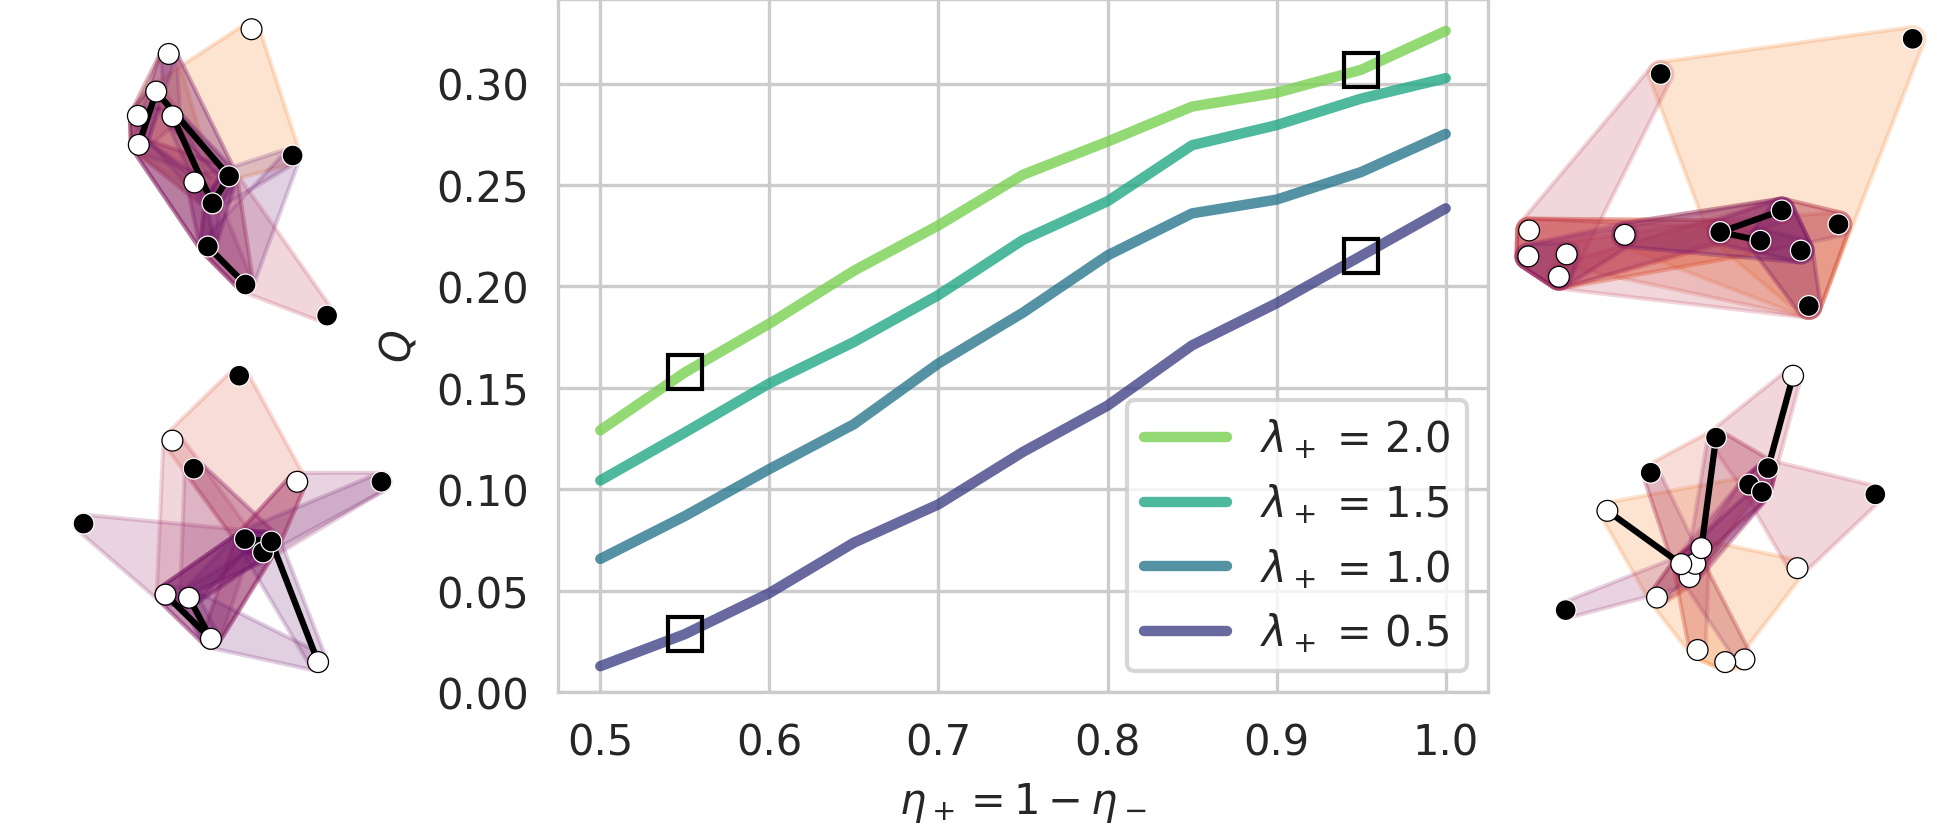
\includegraphics[width=0.48\textwidth]{../fig/community-structure-sims-combined.png}
%DIFDELCMD <         %%%
\DIFdelendFL \DIFaddbeginFL 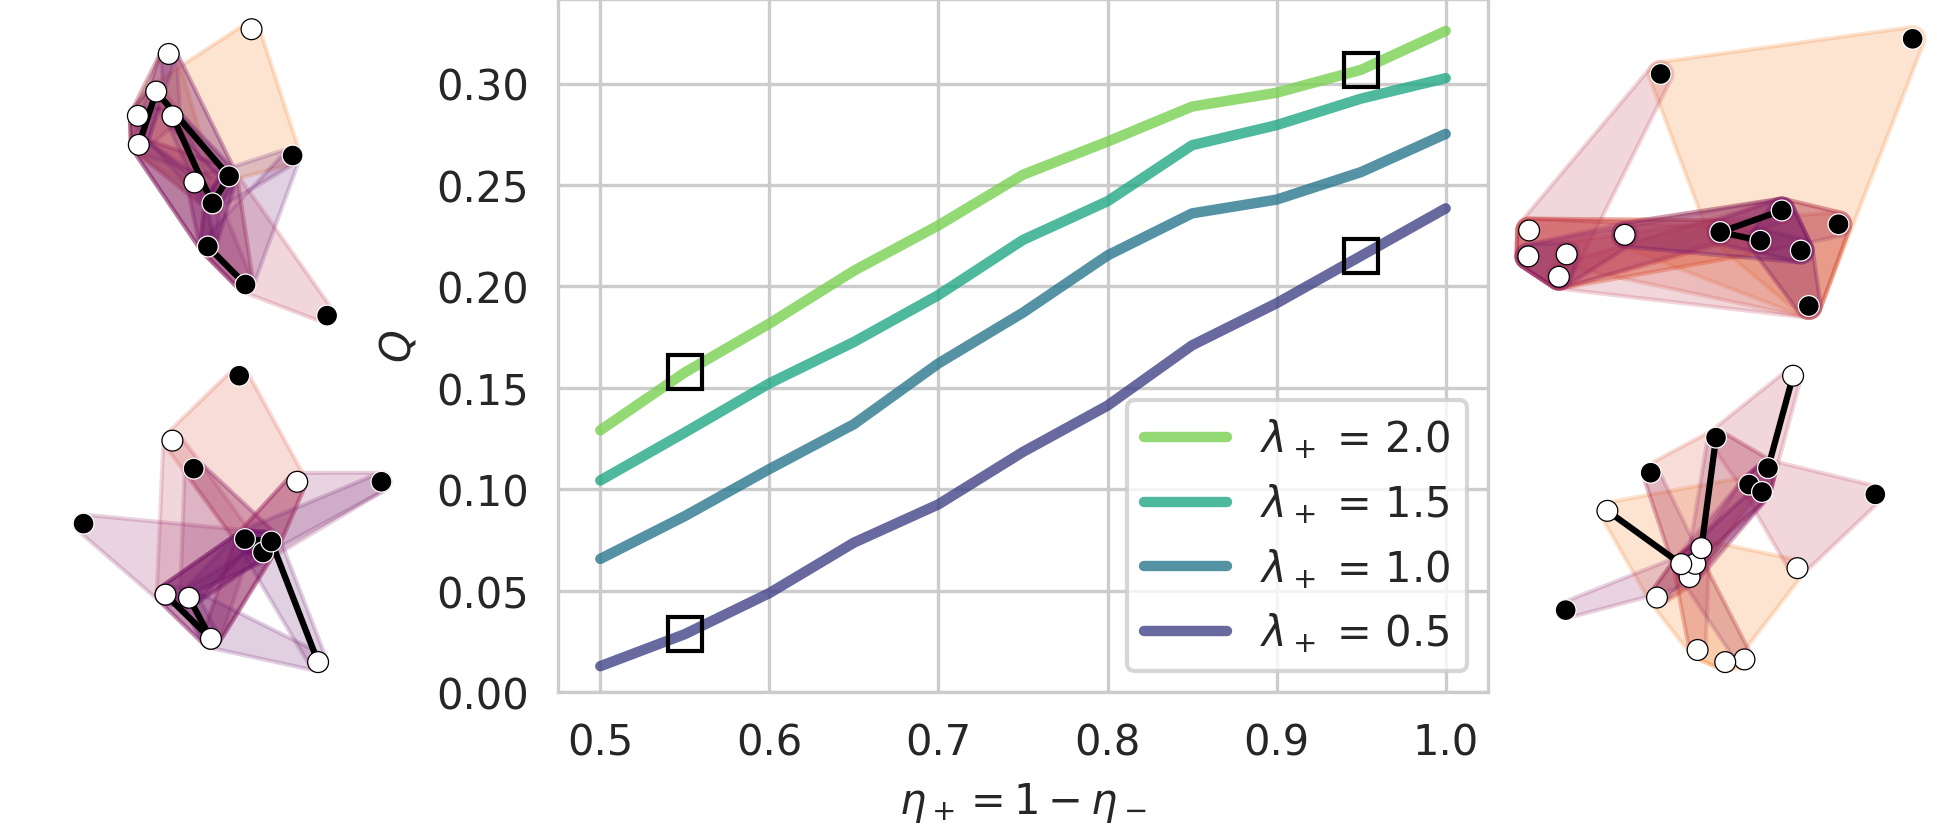
\includegraphics[width=0.495\textwidth]{../fig/community-structure-sims-combined.png}
        \DIFaddendFL \caption{
            Suite of model simulations illustrating the dependence of community structure, as measured by clique-projection modularity $Q$, on the \model{} parameters. 
            The parameters $\opp{\extantrate} = 0.5$ $\same{\novelrate{}} = 0.2$, and $\opp{\novelrate{}} = 0.1$ are held fixed. 
            Each line corresponds to a different value of $\same{\extantrate{}}$ indicated by the legend.
            Along the horizontal axis, we vary $\same{\copyrate{}}$ and set $\opp{\copyrate{}} = 1 - \same{\copyrate{}}$. 
            Each parameter combination is simulated $100$ times for $1,000$ timesteps. 
            On either side of the plot, we show small hypergraphs sampled from parameter combinations indicated by the square markers \DIFaddbeginFL \DIFaddFL{for illustration}\DIFaddendFL .
        }\label{fig:community-structure-illustration}
    \end{figure}
\DIFdelbegin %DIFDELCMD < \frannie{Labels within the figure use old notation.  $Eta_+$, $Eta_-$ and $\lambda_+$ need to be changed to current notation}
%DIFDELCMD < %%%
\DIFdelend 



    \Cref{fig:community-structure-illustration} illustrates the role of the model parameters in tuning the community structure of realized hypergraphs. 
    We measure community structure by computing Newman-Girvan modularity \cite{newman2004finding} on the \DIFaddbegin \DIFadd{weighted }\DIFaddend clique-projection of the hypergraph. 
    \DIFaddbegin \DIFadd{We also show several sample hypergraphs at different parameter combinations for visual illustration. 
    }\DIFaddend For fixed $\opp{\extantrate}$, $\same{\novelrate{}}$, and $\opp{\novelrate{}}$, increasing the difference $\same{\copyrate{}} - \opp{\copyrate{}}$ leads to higher modularity, as does increasing $\same{\extantrate{}}$.
    Hypergraphs sampled from our model using high values of $\same{\copyrate{}}$ and $\same{\extantrate{}}$ tend to have label-homogeneous cores of densely overlapping hyperedges, which are weakly connected to one another by edges with more heterogeneous label compositions.
    Hypergraphs with lower values of $\same{\copyrate{}}$ and $\same{\extantrate{}}$ tend to have less-structured distributions of labels over hyperedges. 
\DIFdelbegin %DIFDELCMD < \frannie{Do $\opp{\copyrate{}}$ and $\opp{\extantrate{}}$ matter here?  Is the difference what's important?}
%DIFDELCMD < %%%
\DIFdelend 



\subsection{Asymptotic Properties} \label{sec:asymptotics}

    \subsubsection{Joint Distribution of Labels in Edges} \label{sec:joint-distribution}

    \begin{figure*}[t]
        \centering
        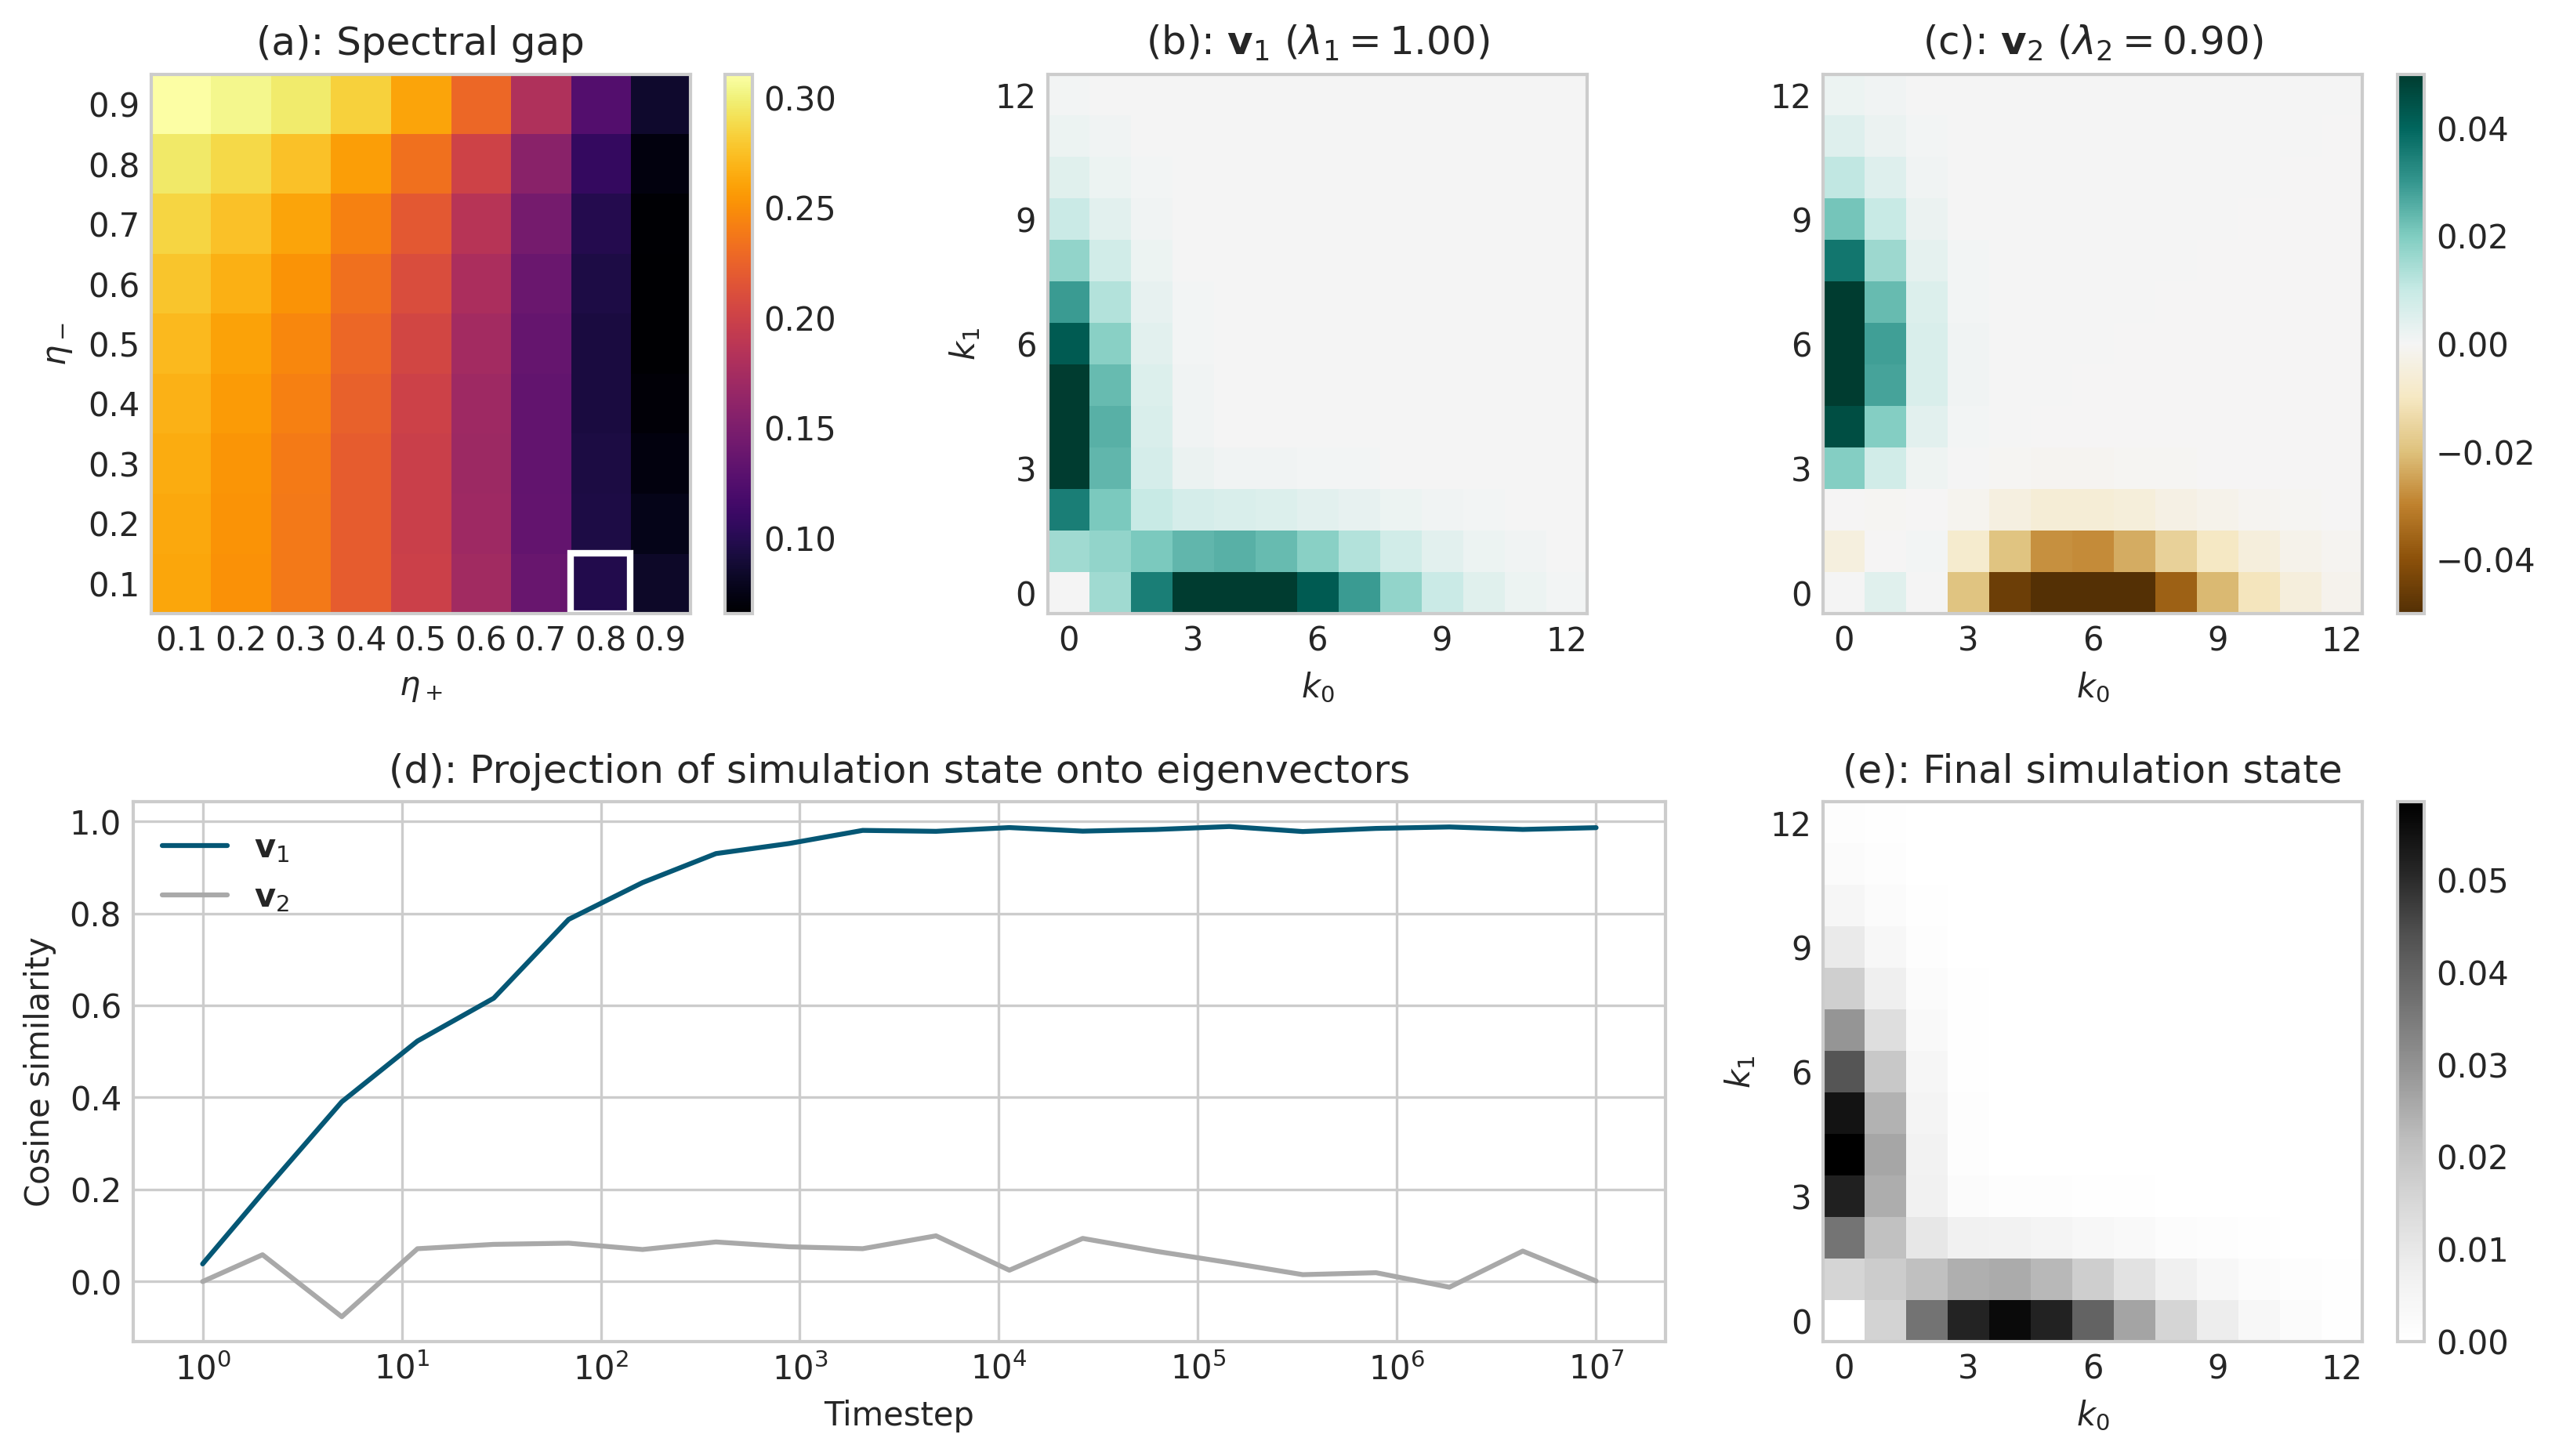
\includegraphics[width=1\textwidth]{../fig/linear_map_eigenvectors.png}
        \caption{
            \DIFdelbeginFL \DIFdelFL{Visualization of the }\DIFdelendFL \DIFaddbeginFL \DIFaddFL{Illustrative }\DIFaddendFL long-run dynamics of our model\DIFdelbeginFL \DIFdelFL{, for parameters}\DIFdelendFL .
            (a): Spectral gap $1 - \lambda_2$ of the linear map $T$ as a function of $\same{\copyrate{}}$ and $\opp{\copyrate{}}$ for fixed parameter values $\same{\extantrate{}} = 0.5$, \DIFdelbeginFL \DIFdelFL{$\opp{\extantrate{}} = \opp{\novelrate{}}3$}\DIFdelendFL \DIFaddbeginFL \DIFaddFL{$\opp{\extantrate{}} = 0.2$}\DIFaddendFL , $\same{\novelrate{}} = 0.4$ and $\opp{\novelrate{}} = 0.2$. 
            The highlighted values $\same{\copyrate{}} = 0.8$ and $\opp{\copyrate{}} = 0.1$ are used in the remainder of the visualization. 
            (b): Leading eigenvector $\mathbf{v}_1$ of $T$, describing the stationary joint distribution $\at{\jointdist}{\infty} \paren{k_0, k_1}$ of label counts in edges.
            (c): Second eigenvector $\mathbf{v}_2$ of $T$. 
            The transients of the model dynamics are dominated by the subspace spanned by $\mathbf{v}_1$ and $\mathbf{v}_2$. 
            (d): Euclidean projections of the simulated joint distribution $\at{\jointdist}{t} \paren{k_0, k_1}$ onto the eigenvectors $\mathbf{v}_1$ and $\mathbf{v}_2$ during a simulation run with $10^7$ timesteps. 
            At each time point, we aggregate the most recent $1,000$ edges to compute the joint distribution in order to approximate an ``instantaneous'' simulation state. 
            (e): Empirical joint distribution $\at{\jointdist}{t} \paren{k_0, k_1}$ aggregated across $10^7$ timesteps. 
        \DIFdelbeginFL %DIFDELCMD < \phil{Frannie and Violet both, I'd like some feedback from you on whether this figure and accompanying discussion seem valuable in proportion to the space they occupy in the paper so far.}
%DIFDELCMD <         %%%
\DIFdelendFL }
        \label{fig:dynamics-eigenvectors}
    \end{figure*}
\DIFdelbegin %DIFDELCMD < \frannie{Awkward sentence (visualization of the long-run dynamics of our model, for parameters) in caption.  Not sure what it is trying to say}
%DIFDELCMD <     \frannie{Typo in caption of panel (a)?  $\opp{\extantrate{}} = \opp{\novelrate{}}3$?  }
%DIFDELCMD < %%%
\DIFdelend 

    Many asymptotic properties of our \model{} model can be described in terms of the joint distribution \DIFdelbegin \DIFdel{$p_{K_0, K_1}(k_0, k_1)$ of nodes of labels }\DIFdelend \DIFaddbegin \DIFadd{$\jointdist(k_0, k_1)$ of node labels in an edge; here $\jointdist(k_0, k_1)$ gives the probability that an edge selected uniformly at random from $\edges$ contains exactly $k_0$ nodes of label }\DIFaddend 0 and \DIFdelbegin \DIFdel{1 in a uniformly random edge. 
    This }\DIFdelend \DIFaddbegin \DIFadd{$k_1$ nodes of label 1.
    Under the $t\rightarrow \infty$ limit this }\DIFaddend joint distribution can be obtained as the leading eigenvector of a linear map\DIFdelbegin \DIFdel{, as we now describe}\DIFdelend . 
    Let $\at{\jointdist}{t}(k_0, k_1)$ be the joint distribution of label counts in a uniformly random edge after $t$ timesteps\DIFaddbegin \DIFadd{, and let $\jointdist(k_0, k_1) = \at{\jointdist}{\infty} \paren{k_0, k_1}$ be the stationary distribution}\DIFaddend .
    Then, the probability \DIFdelbegin \DIFdel{$q(k_0', k_1')$ }\DIFdelend \DIFaddbegin \DIFadd{$r(k_0', k_1')$ }\DIFaddend of realizing an edge with $k_0'$ nodes of label 0 and $k_1'$ nodes of label 1 \DIFdelbegin \DIFdel{at time }\DIFdelend \DIFaddbegin \DIFadd{in timestep }\DIFaddend $t+1$ is given by 
    \begin{align*}
        \DIFdelbegin \DIFdel{q}\DIFdelend \DIFaddbegin \DIFadd{r}\DIFaddend (k_0', k_1') = \sum_{k_0, k_1} T(k_0', k_1' | k_0, k_1)\at{\jointdist}{t}(k_0, k_1)  \;,
    \end{align*}
    where $T(k_0', k_1' | k_0, k_1)$ gives the probability that the edge $e$ realized in step $t+1$ has $k_0'$ nodes of label 0 and $k_1'$ nodes of label 1 given that the edge $f$ sampled to form $e$ has $k_0$ nodes of label 0 and $k_1$ nodes of label 1.
    At stationarity, we must have \DIFdelbegin \DIFdel{$q(k_0', k_1') = \at{\jointdist}{t}(k_0', k_1') = \at{\jointdist}{t+1} \paren{k_0', k_1'}$}\DIFdelend \DIFaddbegin \DIFadd{$r(k_0', k_1') = \at{\jointdist}{t}(k_0', k_1') = \jointdist \paren{k_0', k_1'}$}\DIFaddend , so the stationarity condition can be obtained by solving the linear system 
    \begin{align*}
        \DIFdelbegin %DIFDELCMD < \at{\jointdist}{t+1} %%%
\DIFdelend \DIFaddbegin \jointdist \DIFaddend \paren{k_0', k_1'} = \sum_{k_0, k_1} T(k_0', k_1' | k_0, k_1)\DIFdelbegin %DIFDELCMD < \at{\jointdist}{t} %%%
\DIFdelend \DIFaddbegin \jointdist \DIFaddend \paren{k_0, k_1}  \;.
    \end{align*}
    The stationary joint distribution \DIFdelbegin \DIFdel{$\at{\jointdist}{\infty} \paren{k_0, k_1}$ }\DIFdelend \DIFaddbegin \DIFadd{$\jointdist \paren{k_0, k_1}$ }\DIFaddend is therefore given by the leading eigenvector of the doubly-indexed matrix $T$ with entries $T(k_0', k_1' | k_0, k_1)$. 
    The entries of this matrix \DIFdelbegin \DIFdel{can be computed analytically}\DIFdelend \DIFaddbegin \DIFadd{follow from the parametric probability descriptions used to define the }\model{} \DIFadd{model}\DIFaddend .
    Conditional on choosing an edge \DIFdelbegin \DIFdel{$f$ }\DIFdelend \DIFaddbegin \DIFadd{$\seededge$ }\DIFaddend with $k_0$ nodes of label 0 and $k_1$ nodes of label 1, a node of label $z$ is selected as the \DIFdelbegin \DIFdel{seed node $u$ }\DIFdelend \DIFaddbegin \DIFadd{focal node $\focalnode$ }\DIFaddend with probability $\frac{k_z}{k_0 + k_1}$.
    Then, the number of nodes of labels $z$ and $\bar{z}$ in \DIFdelbegin \DIFdel{$e$ }\DIFdelend \DIFaddbegin \DIFadd{$\newedge$ }\DIFaddend have distributions
    \begin{align*}
        k_z' &\sim 1 + \text{Binom}\paren{k_z - 1, \same{\copyrate{}}} + \text{Poisson}(\same{\extantrate{}} + \same{\novelrate{}}) \;, \\
        k_{\bar{z}}' &\sim \text{Binom}\paren{k_{\bar{z}}, \opp{\copyrate{}}} + \text{Poisson}(\opp{\extantrate{}} + \opp{\novelrate{}}) \;.
    \end{align*}
    The probability of obtaining $k_0'$ nodes of label 0, conditioning on $k_0$ and $k_1$, is 
    \begin{widetext}
        \begin{align*}
            t(k_0' | k_0, k_1) =& \frac{k_0}{k_0 + k_1} \sum_{i=0}^{k_0' - 1} \binom{k_0 - 1}{i} \same{\copyrate{}}^i (1 - \same{\copyrate{}})^{k_0 - 1 - i} 
            e^{-(\same{\extantrate{}} + \same{\novelrate{}})} \frac{(\same{\extantrate{}} + \same{\novelrate{}})^{k_0' - 1 - i}}{(k_0' - 1 - i)!}  + \\ 
            & \frac{k_1}{k_0 + k_1} \sum_{i=0}^{k_0'} \binom{k_0}{i} \opp{\copyrate{}}^i (1 - \opp{\copyrate{}})^{k_0 - i} 
            e^{-(\opp{\extantrate{}} + \opp{\novelrate{}})} \frac{(\opp{\extantrate{}} + \opp{\novelrate{}})^{k_0' - i}}{(k_0' - i)!}\;.
        \end{align*}
    \end{widetext}
    A parallel expression describes $t(k_1' | k_0, k_1)$, and the transition matrix entries are given by the product 
    \begin{align*}
        T(k_0', k_1' | k_0, k_1) = t(k_0' | k_0, k_1) t(k_1' | k_0, k_1) \;.
    \end{align*}
    In \Cref{fig:dynamics-eigenvectors}, we study the dynamics of our \model{} model as described by the matrix $T$. 
    \DIFaddbegin \DIFadd{The spectral gap $1 - \lambda_2$ of $T$ is a measure of the rate of convergence to the stationary distribution $\jointdist \paren{k_0, k_1}$, where $\lambda_2$ is the second-largest eigenvalue of $T$.
    }\DIFaddend For fixed values of the parameters $\same{\extantrate{}}$, $\opp{\extantrate{}}$, $\same{\novelrate{}}$ and $\opp{\novelrate{}}$, the spectral gap $1 - \lambda_2$ of $T$ is highest when $\opp{\copyrate}$ is large and $\same{\copyrate}$ is small. 
    High values of the spectral gap correspond to fast convergence to the stationary distribution \DIFdelbegin \DIFdel{$\at{\jointdist}{\infty} \paren{k_0, k_1}$ }\DIFdelend \DIFaddbegin \DIFadd{$\jointdist \paren{k_0, k_1}$ }\DIFaddend given by the Perron eigenvector $\mathbf{v}_1$ of $T$ with eigenvalue $1$ (panel (b)). 
    We instead illustrate an alternative regime of relatively slow convergence in which $\same{\copyrate}$ is large and $\opp{\copyrate}$ is small.
    In this regime, the simulation may maintain transient dynamics in the direction of the second eigenvector $\mathbf{v}_2$ of $T$ with eigenvalue $\lambda_2 < 1$ (panel (c)) for relatively long periods of time before converging to the stationary distribution. 
    We illustrate this behavior in panel (d), where the system converges relatively slowly to the leading eigenvector $\mathbf{v}_1$ and away from the transient component $\mathbf{v}_2$. 
    The resulting final simulation state matches the stationary distribution \DIFdelbegin \DIFdel{$\at{\jointdist}{\infty} \paren{k_0, k_1}$ }\DIFdelend \DIFaddbegin \DIFadd{$\jointdist \paren{k_0, k_1}$ }\DIFaddend relatively closely (panel (e)).

    \Cref{fig:dynamics-eigenvectors} shows that, when $\same{\copyrate{}}$ is sufficiently large, the stationary distribution \DIFdelbegin \DIFdel{$\at{\jointdist}{\infty} \paren{k_0, k_1}$ }\DIFdelend \DIFaddbegin \DIFadd{$\jointdist \paren{k_0, k_1}$ }\DIFaddend is concentrated on edges in which typical edges have large majorities of nodes with the same label (panel b), \DIFdelbegin \DIFdel{thus displaying a form }\DIFdelend \DIFaddbegin \DIFadd{the signature }\DIFaddend of higher-order \DIFdelbegin \DIFdel{homophily \mbox{%DIFAUXCMD
\cite{laber2026guide}}\hskip0pt%DIFAUXCMD
.
    }\DIFdelend \DIFaddbegin \DIFadd{structural assortativity.
    This distribution is symmetric with respect to the two node labels, however, indicating that although local edges may have dominant majority labels, the long-run dynamics converge to equal global label populations.  
    }\DIFaddend The second eigenvector $v_2$ (panel c), however,  is antisymmetric, describing a transient in which a single label group tends to dominate most edges. 
    When $\same{\copyrate{}}$ is sufficiently large, the spectral gap $1 - \lambda_2$ is small (panel a), indicating that this transient decays slowly and that the system may be dominated by edges with a single majority label for relatively long periods of time before equilibrating to the leading eigenvector (panels \DIFdelbegin \DIFdel{d and e)}\DIFdelend \DIFaddbegin \DIFadd{(d-e))}\DIFaddend .
    This behavior suggests that, although the \model{} model ultimately converges to a stationary state with symmetry between the two node labels, it can also serve through its transients as a reasonable generative model of systems with label asymmetry. 

    

\subsubsection{Degree Distribution} \label{sec:degree-distribution}

    \DIFdelbegin \DIFdel{The degree distribution of a hypergraph generated from the }\DIFdelend \DIFaddbegin \DIFadd{One model feature we can obtain from the stationary joint distribution $\jointdist \paren{k_0, k_1}$ is the asymptotic degree distribution generated from }\DIFaddend \model{}\DIFdelbegin \DIFdel{model follows an asymptotic }\DIFdelend \DIFaddbegin \DIFadd{.
    This asymptotic distribution a asymptotic }\DIFaddend power law with an exponent which can be computed in closed form from the model parameters and the stationary joint distribution \DIFdelbegin \DIFdel{$\at{\jointdist}{\infty} \paren{k_0, k_1}$}\DIFdelend \DIFaddbegin \DIFadd{$\jointdist \paren{k_0, k_1}$}\DIFaddend . 
    Our derivation is similar to that of He et al. \cite{heEdgeCorrelationsLink2025}, which in turn is based on a derivation by Mitzenmacher \cite{mitzenmacherBriefHistoryGenerative2004}. 
    The argument requires a mean-field assumption: 
    when a node $\focalnode$ is selected from edge $\seededge$ in the edge-sampling step, the degree $d$ of $\focalnode$ is independent of the ratio $\frac{k_0}{k}$ of label-0 nodes in the edge $\seededge$ sampled to form the new edge $\newedge$.
    \DIFdelbegin %DIFDELCMD < 

%DIFDELCMD <     %%%
\DIFdelend Under this assumption, it is possible to show that the degree distribution follows a power law with exponent
    \begin{align}
        \zeta &= 1 + \DIFdelbegin \DIFdel{\frac{\brackets{k}}{1 + \same{\copyrate{}}(\rho_{00} + \rho_{11} - 1) + 2\opp{\copyrate{}} \rho_{01}} }\DIFdelend \DIFaddbegin \DIFadd{\frac{\brackets{k_0} + \brackets{k_1}}{1 + \same{\copyrate{}}(\moment_{00} + \moment_{11} - 1) + 2\opp{\copyrate{}} \moment_{01}} }\DIFaddend \label{eq:power-law-exponent}\\ 
        \DIFdelbegin \DIFdel{\rho}\DIFdelend \DIFaddbegin \moment\DIFaddend _{ij} &= \brackets{\frac{k_i k_j}{k}} \;. \nonumber
    \end{align}
    In the expression for \DIFdelbegin \DIFdel{$\rho_{ij}$ }\DIFdelend \DIFaddbegin \DIFadd{$\moment_{ij}$ }\DIFaddend (and for \DIFdelbegin \DIFdel{$\brackets{k}$}\DIFdelend \DIFaddbegin \DIFadd{$\brackets{k_i}$}\DIFaddend ) the expectation is taken with respect to the stationary joint distribution \DIFdelbegin \DIFdel{$\at{\jointdist}{\infty} \paren{k_0, k_1}$.
    Here, $\novelrate{}$ can be interpreted as the expected number of novel nodes added per new edge, while $\expectedcopiednodes{}$ can be interpreted as the expected number of nodes copied into a new edge from the sampled edge, normalized by the average degree of a node in the hypergraph.
    }\DIFdelend \DIFaddbegin \DIFadd{$\jointdist \paren{k_0, k_1}$.
    }\DIFaddend A derivation of this result and a computational illustration are provided in \DIFaddbegin \DIFadd{Appendix }\DIFaddend \Cref{sec:degree-distribution-appendix} and \Cref{fig:degrees}. 

\section{Model Inference} \DIFaddbegin \label{sec:inference}
\DIFaddend 

    In this section, we consider the problems of \emph{parameter inference} (learning $\paramvector$ given $\hypergraph$ and $\vz$) and \emph{community detection} (learning $\vz$ given $\hypergraph$ and $\paramvector$). 


\subsection{Parameter Estimation via Stochastic EM} \label{sec:sem}

    We first consider the problem of learning the parameter vector $\paramvector = (\same{\copyrate{}}, \opp{\copyrate{}}, \same{\extantrate{}}, \opp{\extantrate{}}, \same{\novelrate{}}, \opp{\novelrate{}})$ given an observed hypergraph $\hypergraph$ with sequential edge indices and known node labels $\vz$.
    We aim to do this via maximum-likelihood estimation. 
    Computing the complete data likelihood requires marginalizing over the model latent variables, which in this case are the edge $f$ and node $u$ selected at each timestep of the growth model to form the new edge $e$. 
    For $\newedge \in \edges$, let $t_\newedge$ denote the time at which $\newedge$ was added to the hypergraph.
    We say that $\seededge \prec \newedge$ if $t_{\seededge} < t_{\newedge}$. 
    \DIFdelbegin %DIFDELCMD < \frannie{Might be helpful to broaden $\prec$ to $t_f < t_e$ and $|f\cap e| \neq 0$. Would incorporate logic in note after \cref{eq:bayes}}
%DIFDELCMD <     %%%
\DIFdelend Then, the complete data likelihood can be written 
    \DIFaddbegin \begin{widetext}
    \DIFaddend \begin{align}
        \DIFdelbegin %DIFDELCMD < \prob%%%
\DIFdelend \DIFaddbegin \lik\DIFaddend (\hypergraph, \vz \DIFdelbegin \DIFdel{| }\DIFdelend \DIFaddbegin \DIFadd{; }\DIFaddend \paramvector) = \prod_{\newedge \in \edges} \sum_{\seededge \prec \newedge} \sum_{\focalnode \in \seededge} \DIFdelbegin \DIFdel{p}\DIFdelend \DIFaddbegin \lik\DIFaddend (\newedge\DIFaddbegin \DIFadd{, }\vz\DIFadd{'_e }\DIFaddend | \seededge, \focalnode, \DIFdelbegin %DIFDELCMD < \vz%%%
\DIFdel{, }\DIFdelend \DIFaddbegin \at{\vz}{t_e-1}\DIFadd{; }\DIFaddend \paramvector) \DIFdelbegin \DIFdel{p}\DIFdelend \DIFaddbegin \lik\DIFaddend (\seededge,\focalnode | \DIFdelbegin %DIFDELCMD < \edges%%%
\DIFdel{^{t - 1}}\DIFdelend \DIFaddbegin \at{\edges}{t_e-1}\DIFaddend , \DIFdelbegin %DIFDELCMD < \vz%%%
\DIFdel{, }\DIFdelend \DIFaddbegin \at{\vz}{t_e-1}\DIFadd{; }\DIFaddend \paramvector) \;\DIFdelbegin \DIFdel{. }\DIFdelend \DIFaddbegin \DIFadd{, }\DIFaddend \label{eq:likelihood}
    \end{align}
\DIFdelbegin \DIFdel{For notational simplicity, we have suppressed the additional entries of $\vz$ introduced by the novel node addition step.
    The requirement }\DIFdelend \DIFaddbegin \end{widetext}
    \DIFadd{where $\at{\vz}{t_e-1}$ is the vector of node labels immediately before $e$ was added, and $\vz'_e$ is the vector of node labels added with edge $e$ at time $t_e$.
    %DIF >  For notational simplicity, we'll omit the time indices on $\vz$ and the additional labels $\vz'_e$ in the remainder of our discussion. 
    The term $\lik(\seededge,\focalnode | \at{\edges}{t_e-1}, \at{\vz}{t_e-1}; \paramvector)$ gives the likelihood of selecting edge $\seededge$ and node $\focalnode$ at time $t - 1$; its value is $\frac{1}{\abs{\seededge}\at{m}{t-1}}$ if $\seededge \in \at{\edges}{t_e-1}$ and $0$ otherwise, where $\at{m}{t-1} = \abs{\at{\edges}{t_e-1}}$ is the number of edges at time $t - 1$.
    The term $\lik(\newedge, \vz'_e | \seededge, \focalnode, \at{\vz}{t_e-1}; \paramvector)$ gives the likelihood of realizing edge $\newedge$ and the associated new node labels $\vz'_e$ given that edge $\seededge$ and node $\focalnode$ were selected at time $t - 1$.
    A helpful note for computation is that $\lik(\newedge, \vz'_e | \seededge, \focalnode, \at{\vz}{t_e-1}; \atalg{\hat{\paramvector}}{\ell}) = 0$ if either $\focalnode \notin \newedge\cap \seededge$ or $\seededge\not\prec \newedge$. 
}


    \DIFadd{The requirement in \mbox{%DIFAUXCMD
\cref{eq:likelihood} }\hskip0pt%DIFAUXCMD
}\DIFaddend to sum over the latent variables at each timestep implies a computational cost to evaluate \DIFdelbegin \DIFdel{$\prob(\hypergraph, \vz | \paramvector)$ }\DIFdelend \DIFaddbegin \DIFadd{$\lik(\hypergraph, \vz ; \paramvector)$ }\DIFaddend (or its derivatives) \DIFdelbegin \DIFdel{, }\DIFdelend which is quadratic in the number of edges \DIFaddbegin \DIFadd{$m$}\DIFaddend , making direct optimization of the likelihood expensive for data sets of even modest size. 
    Batch expectation-maximization \cite{dempster1977maximum}  is an alternative approach which maximizes the likelihood without explicitly computing \cref{eq:likelihood}, but even this approach requires forming a belief distribution over the values of all latent variables at each timestep, which again incurs quadratic cost \DIFaddbegin \DIFadd{per iteration}\DIFaddend . 

    We therefore use a stochastic expectation-maximization (SEM) algorithm \cite{cappeOnLineExpectationMaximization2009} to estimate the parameters $\paramvector$.
    Each iteration of \DIFdelbegin \DIFdel{the SEM algorithm }\DIFdelend \DIFaddbegin \DIFadd{SEM }\DIFaddend consists of two steps: the \DIFaddbegin \DIFadd{stochatic }\DIFaddend E-step, in which \DIFaddbegin \DIFadd{noisy }\DIFaddend exponentially weighted moving averages of the sufficient statistics are calculated using the current parameter estimates, and the \DIFaddbegin \DIFadd{stochastic }\DIFaddend M-step, in which the parameter estimates are updated using the expected sufficient statistics. 

    %DIF <  Suppose we have an observed variable $x$ and a hidden variable $h$. Let $f(x_i, h_i)$ be a function which computes a sufficient statistic for each of the parameters in $\theta$ and let $F_i(\hat{\theta}) = \mathbb{E}[f(x_i, h_i) | x_i]$ be the function which computes the expected sufficient statistic values given an observed $x_i$. Let $g$ be a function which computes the maximum likelihood estimate of $\theta$ from the sufficient statistics. Fix a sequence of learning rates $\ell^{(1)}, \ldots, \ell^{(t)}$. Each iteration, $t$, of SEM proceeds as follows.
    \DIFdelbegin %DIFDELCMD < 

%DIFDELCMD < %%%
%DIF <  \textbf{E step:} Sample an observation $x_i$ from the data uniformly at random. Compute the expected sufficient statistics $F_i(\hat{\theta}^{(t - 1)})$ using the randomly selected data point $x_i$ and the parameter estimates $\hat{\theta}^{(t - 1)}$ from the previous timestep. Generate an new estimate of sufficient statistics $s^{(t)}$ according to the update rule: $s^{(t)} = (1 - \ell^{(t)}) s^{(t - 1)} + \ell^{(t)}F_i(\hat{\theta}^{(t - 1)})$.
    %DIFDELCMD < 

%DIFDELCMD < %%%
%DIF <  \textbf{M step:} Compute the new parameter estimates $\hat{\theta}^{(t)}$ from the updated sufficient statistics:
%DIF <  $\hat{\theta}^{(t)} = g(s^{(t)})$.
    %DIFDELCMD < 

%DIFDELCMD < %%%
%DIF <  \subsubsection{Description of SEM on hypergraphs}
%DIF <  We use an SEM algorithm to estimate the parameters $\theta = (\same{\copyrate{}}, \opp{\copyrate{}}, \same{\extantrate{}}, \opp{\extantrate{}}, \same{\novelrate{}}, \opp{\novelrate{}})$ used to generate a hypergraph $\mathcal{H}$ via the [MODEL NAME] model. 
%DIFDELCMD < 

%DIFDELCMD < %%%
\DIFdelend To initialize the SEM algorithm, we \DIFaddbegin \DIFadd{first }\DIFaddend initialize a vector \DIFdelbegin \DIFdel{$\at{\sufficientstatsvec}{0}$ }\DIFdelend \DIFaddbegin \DIFadd{$\atalg{\sufficientstatsvec}{0}$ }\DIFaddend of sufficient statistics to arbitrary values; in our model, there \DIFdelbegin \DIFdel{is a sufficient statistic for each parameter}\DIFdelend \DIFaddbegin \DIFadd{are two sufficient statistics per copy parameter and one sufficient statistic per each of the four addition parameters, so $\sufficientstatsvec$ has length $8$.
    From $\atalg{\sufficientstatsvec}{0}$, we compute an initial estimate of the parameter vector $\atalg{\hat{\paramvector}}{0} = g(\atalg{\sufficientstatsvec}{0})$ via a function $g$ which maps sufficient statistics to parameter estimates; details on both the sufficient statistics $\sufficientstatsvec$ and the mapping $g$ are provided in \mbox{%DIFAUXCMD
\Cref{sec:sufficient-statistics}}\hskip0pt%DIFAUXCMD
}\DIFaddend .
    We then update a moving average of $\sufficientstatsvec$ as follows. 
    In each algorithmic step $\ell$, we pick an edge $e$ uniformly at random from $\hypergraph$. 
    Then, given current estimates \DIFdelbegin \DIFdel{$\at{\hat{\paramvector}}{\ell}$}\DIFdelend \DIFaddbegin \DIFadd{$\atalg{\hat{\paramvector}}{\ell}$}\DIFaddend , we form a belief distribution over the latent identities of $\seededge \in \edges$ and $\focalnode \in \seededge$ which could have been selected in the edge-copying step to form $\newedge$. 
    \DIFdelbegin \DIFdel{Given $\newedge$, the probability that $\seededge$ and $\focalnode$ were selected can be computed in closed form. 
Let $\at{m}{t-1}$ denote the size of the edge set at time $t - 1$.
}%DIFDELCMD < 

%DIFDELCMD < %%%
\DIFdel{We have 
}\begin{align*}
    \DIFdel{p(\seededge, \focalnode | \at{\edges}{t-1}, \vz, \at{\hat{\paramvector}}{\ell}) = \frac{1}{\abs{\seededge}\at{m}{t-1}} \triangleq r_{t-1}(\seededge) \;,
}\end{align*}%DIFAUXCMD
\DIFdel{so }\DIFdelend \DIFaddbegin \DIFadd{Using }\DIFaddend Bayes' rule\DIFdelbegin \DIFdel{gives 
}\begin{align*}
    \DIFdel{p(\seededge,\focalnode | \newedge, \at{\hat{\paramvector}}{\ell}) = \frac{p(\newedge | \seededge, \focalnode, \vz, \at{\hat{\paramvector}}{\ell}) r_{t-1}(\seededge)}{\sum_{\seededge' \prec \newedge} \sum_{\focalnode' \in \seededge'} p(\newedge | \seededge', \focalnode', \vz, \at{\hat{\paramvector}}{\ell}) r_{t-1}(\seededge') } \;. %DIFDELCMD < \label{eq:bayes}%%%
}\end{align*}%DIFAUXCMD
\DIFdelend \DIFaddbegin \DIFadd{, this probability is 
    }\begin{widetext}
    \begin{align}
        \DIFadd{\lik(\seededge,\focalnode | \newedge, \vz'_e; \atalg{\hat{\paramvector}}{\ell}) = \frac{\lik(\newedge, \vz'_e | \seededge, \focalnode, \at{\vz}{t_e-1}; \atalg{\hat{\paramvector}}{\ell}) \abs{\seededge}^{-1}}{\sum_{\seededge' \prec \newedge} \sum_{\focalnode' \in \seededge'} \lik(\newedge, \vz'_e | \seededge', \focalnode', \at{\vz}{t_e-1}; \atalg{\hat{\paramvector}}{\ell}) \abs{\seededge'}^{-1} } \;. \label{eq:bayes}
    }\end{align}\DIFaddend 
    \DIFdelbegin \DIFdel{A helpful note for computation is 
    that $p(\newedge|\seededge, \focalnode, \vz, \at{\hat{\paramvector}}{\ell}) = 0$ if either $\focalnode \notin \newedge\cap \seededge$ or $\seededge\not\prec \newedge$. 
}\DIFdelend \DIFaddbegin \end{widetext}
    \DIFaddend We then form the vector of expected sufficient statistics 
    \begin{align}
        s' = \sum_{\seededge \prec \newedge} \sum_{\focalnode \in \seededge\cap \newedge} \DIFdelbegin \DIFdel{p}\DIFdelend \DIFaddbegin \lik\DIFaddend (\seededge, \focalnode | \newedge, \DIFdelbegin %DIFDELCMD < \at{\hat{\paramvector}}{\ell}%%%
\DIFdelend \DIFaddbegin \vz\DIFadd{'_e; }\atalg{\hat{\paramvector}}{\ell}\DIFaddend ) \DIFdelbegin \DIFdel{\sigma}\DIFdelend \DIFaddbegin \vsigma\DIFaddend (\newedge, \seededge, \focalnode, \vz) \;, \label{eq:sufficient-stats-update}
    \end{align}
    where \DIFdelbegin \DIFdel{$\sigma(\newedge, \seededge, \focalnode, \vz)$ }\DIFdelend \DIFaddbegin \DIFadd{$\vsigma(\newedge, \seededge, \focalnode, \vz)$ }\DIFaddend is the vector of sufficient statistics for the parameters $\paramvector$ given $\newedge$, $\seededge$, $\focalnode$, and $\vz$.
    The entries of \DIFdelbegin \DIFdel{$\sigma(\newedge, \seededge, \focalnode, \vz)$ }\DIFdelend \DIFaddbegin \DIFadd{$\vsigma(\newedge, \seededge, \focalnode, \vz)$ }\DIFaddend can be computed as functions of the node labels in $\newedge$ and $\seededge$; we supply explicit formulae in \Cref{sec:sufficient-statistics}. 
    We then perform the update 
    \begin{align*}
        \DIFdelbegin %DIFDELCMD < \at{\sufficientstatsvec}{\ell+1} %%%
\DIFdelend \DIFaddbegin \atalg{\sufficientstatsvec}{\ell+1} \DIFaddend = (1 - \DIFdelbegin %DIFDELCMD < \lr%%%
\DIFdel{^{(\ell)}}\DIFdelend \DIFaddbegin \atalg{\lr}{\ell} \DIFaddend )\DIFdelbegin %DIFDELCMD < \at{\sufficientstatsvec}{\ell} %%%
\DIFdelend \DIFaddbegin \atalg{\sufficientstatsvec}{\ell} \DIFaddend + \DIFdelbegin %DIFDELCMD < \lr%%%
\DIFdel{^{(\ell)} }\DIFdelend \DIFaddbegin \atalg{\lr}{\ell} \DIFaddend \sufficientstatsvec' \;,
    \end{align*}
    where \DIFdelbegin \DIFdel{$\lr^{(\ell)}$ }\DIFdelend \DIFaddbegin \DIFadd{$\atalg{\lr}{\ell}$ }\DIFaddend is the learning rate at \DIFdelbegin \DIFdel{step }\DIFdelend \DIFaddbegin \DIFadd{iteration }\DIFaddend $\ell$; we use an exponentially decaying learning rate in our experiments.
    Our \DIFaddbegin \DIFadd{new }\DIFaddend estimate of the parameter vector $\paramvector$ is then given by a function \DIFdelbegin \DIFdel{$\at{\hat{\paramvector}}{\ell+1} = g(\at{\sufficientstatsvec}{\ell+1})$ }\DIFdelend \DIFaddbegin \DIFadd{$\atalg{\hat{\paramvector}}{\ell+1} = g(\atalg{\sufficientstatsvec}{\ell+1})$ }\DIFaddend of the sufficient statistics, which we also supply in \Cref{sec:sufficient-statistics}.
    \Cref{alg:sem} summarizes \DIFdelbegin \DIFdel{the steps of this algorithm}\DIFdelend \DIFaddbegin \DIFadd{this process}\DIFaddend . 
    Our version of the algorithm uses an online computation of $\sufficientstatsvec'$, which allows us to perform the double-sum appearing in \cref{eq:sufficient-stats-update,eq:bayes} only once, and without explicitly storing the resulting belief distribution at any point.  



    \begin{algorithm}[H]
        \caption{\model{} SEM Update Step}\label{alg:sem}
        \begin{algorithmic}
        \Require $\hypergraph = \paren{\nodes, \edges}$, $\vz$, \DIFdelbegin \DIFdel{$\at{\hat{\paramvector}}{\ell}$, $\at{\sufficientstatsvec}{\ell}$
    }\DIFdelend \DIFaddbegin \DIFadd{$\atalg{\hat{\paramvector}}{\ell}$, $\atalg{\sufficientstatsvec}{\ell}$
        }\DIFaddend \State $e \gets \text{Uniform}(\edges)$
        \State \DIFdelbegin \DIFdel{$a \gets \vzero$
    }\DIFdelend \DIFaddbegin \DIFadd{$\vx \gets \vzero$
        }\DIFaddend \State \DIFdelbegin \DIFdel{$b \gets \vzero$
    }\DIFdelend \DIFaddbegin \DIFadd{$\vy \gets \vzero$
        }\DIFaddend \For{$\seededge \in \edges$}
            \If{$\seededge \prec \newedge$}
                \For{$\focalnode \in \newedge \cap \seededge$}
                    \State \DIFdelbegin \DIFdel{$a \gets a + p(\seededge, \focalnode | \newedge, \at{\hat{\paramvector}}{\ell}) \sigma(\newedge, \seededge, \focalnode, \vz)$
                }\DIFdelend \DIFaddbegin \DIFadd{$\vx \gets \vx + \lik(\seededge, \focalnode | \newedge; \atalg{\hat{\paramvector}}{\ell}) \vsigma(\newedge, \seededge, \focalnode, \vz)$
                    }\DIFaddend \State \DIFdelbegin \DIFdel{$b \gets b + p(\seededge, \focalnode | \newedge, \at{\hat{\paramvector}}{\ell})$
            }\DIFdelend \DIFaddbegin \DIFadd{$\vy \gets \vy + \lik(\seededge, \focalnode | \newedge; \atalg{\hat{\paramvector}}{\ell})$
                }\DIFaddend \EndFor
            \EndIf
        \EndFor
        \State \DIFdelbegin \DIFdel{$\sufficientstatsvec' \gets a / b$
    }\DIFdelend \DIFaddbegin \DIFadd{$\sufficientstatsvec' \gets \vx \oslash \vy$ }\Comment{entrywise division}
        \DIFaddend \State \DIFdelbegin \DIFdel{$\at{\sufficientstatsvec}{\ell+1} \gets (1 - \lr^{(\ell)}) \at{\sufficientstatsvec}{\ell} + \lr^{(\ell)} \sufficientstatsvec'$
    }\DIFdelend \DIFaddbegin \DIFadd{$\atalg{\sufficientstatsvec}{\ell+1} \gets (1 - \atalg{\lr}{\ell} )\atalg{\sufficientstatsvec}{\ell} + \atalg{\lr}{\ell} \sufficientstatsvec'$
        }\DIFaddend \State \DIFdelbegin \DIFdel{$\at{\hat{\paramvector}}{\ell+1} \gets g(\at{\sufficientstatsvec}{\ell+1})$
    }\DIFdelend \DIFaddbegin \DIFadd{$\atalg{\hat{\paramvector}}{\ell+1} \gets g(\atalg{\sufficientstatsvec}{\ell+1})$
        }\DIFaddend \State \Return \DIFdelbegin \DIFdel{$\at{\hat{\paramvector}}{\ell+1}$, $\at{\sufficientstatsvec}{\ell+1}$
    }\DIFdelend \DIFaddbegin \DIFadd{$\atalg{\hat{\paramvector}}{\ell+1}$, $\atalg{\sufficientstatsvec}{\ell+1}$
        }\DIFaddend \end{algorithmic}
    \end{algorithm}


    We perform SEM by repeating \Cref{alg:sem} until a stopping criterion is met. 
    \DIFdelbegin \DIFdel{We }\DIFdelend \DIFaddbegin \DIFadd{For our criterion, we }\DIFaddend define the function 
    \begin{align*}
        h(\DIFdelbegin %DIFDELCMD < \at{\hat{\paramvector}}{\ell}%%%
\DIFdelend \DIFaddbegin \atalg{\hat{\paramvector}}{\ell}\DIFaddend , \DIFdelbegin %DIFDELCMD < \at{\hat{\paramvector}}{\ell'}%%%
\DIFdelend \DIFaddbegin \atalg{\hat{\paramvector}}{\ell'}\DIFaddend ) = \min_{i} \left\{\DIFdelbegin %DIFDELCMD < \abs{\at{\hat{\param}_i}{\ell} - \at{\hat{\param}_i}{\ell'}} %%%
\DIFdelend \DIFaddbegin \abs{\atalg{\hat{\param}_i}{\ell} - \atalg{\hat{\param}_i}{\ell'}} \DIFaddend - \epsilon_\mathrm{rel} - \epsilon_\mathrm{abs} \DIFdelbegin %DIFDELCMD < \at{\hat{\param}_i}{\ell'}%%%
\DIFdelend \DIFaddbegin \atalg{\hat{\param}_i}{\ell'}\DIFaddend \right\} \;.
    \end{align*}
    The function $h$ here can be viewed as combining absolute and relative error tolerances, enabling the algorithm to declare convergence even in cases when the parameter estimates are near zero. 
    In our implementation, we declare convergence at timestep $\ell$ when \DIFdelbegin \DIFdel{$h(\at{\hat{\paramvector}}{\ell}, \at{\hat{\paramvector}}{\ell'}) \geq 0$ }\DIFdelend \DIFaddbegin \DIFadd{$h(\atalg{\hat{\paramvector}}{\ell}, \atalg{\hat{\paramvector}}{\ell'}) \geq 0$ }\DIFaddend for all $\ell'$ in the most recent 800 iterations of the algorithm\DIFdelbegin \DIFdel{.
In our experiments we used $\epsilon_\mathrm{rel} = 0.01$ and $\epsilon_\mathrm{abs} = 0.015$}\DIFdelend \DIFaddbegin \DIFadd{, with tolerances $\epsilon_\mathrm{rel}$ and $\epsilon_\mathrm{abs}$}\DIFaddend .

\subsection{Community Detection via Simulated Annealing} \label{sec:community-detection}

    We also consider the community detection problem of learning the node labels $\vz$ given an observed hypergraph $\hypergraph$ and a fixed parameter vector $\paramvector$.

    \DIFaddbegin \DIFadd{Since }\DIFaddend \Cref{eq:likelihood} defines a likelihood function over both the parameter vector $\paramvector$ and the node labels $\vz$\DIFdelbegin \DIFdel{.
    This allows us to }\DIFdelend \DIFaddbegin \DIFadd{, we can }\DIFaddend attempt to also learn $\vz$ via maximum-likelihood estimation.
    Unlike in stochastic block model variants in which there are several heuristics with favorable computational properties \cite{newman2016equivalence,chodrowGenerativeHypergraphClustering2021,chodrowNonbacktrackingSpectralClustering2023,ruggeriCommunityDetectionLarge2023,kritschgauCommunityDetectionHypergraphs2024,hood2026broad,li2026higher}, the \DIFaddbegin \DIFadd{edge }\DIFaddend dependence structure encoded by \model{} makes it difficult to apply standard efficient heuristics\DIFdelbegin \DIFdel{; the development of such heuristics would be }\DIFdelend \DIFaddbegin \DIFadd{.
    The development of alternative efficient heuristics is }\DIFaddend an important direction of future work. 
    In \DIFdelbegin \DIFdel{this study}\DIFdelend \DIFaddbegin \DIFadd{our present approach}\DIFaddend , we therefore attempt to learn $\vz$ via simulated annealing \cite{kirkpatrickOptimizationSimulatedAnnealing1983},  \DIFdelbegin \DIFdel{which is }\DIFdelend a general-purpose optimization algorithm \DIFdelbegin \DIFdel{that can be used to approximately maximize the likelihood over $\vz$}\DIFdelend \DIFaddbegin \DIFadd{which is typically used when other heuristics are not available}\DIFaddend . 
    Our primary aim is to demonstrate that likelihood maximization in this model can detect label structure in at least some circumstances where \DIFdelbegin \DIFdel{more standard community detections may fail}\DIFdelend \DIFaddbegin \DIFadd{other community detection methods perform poorly}\DIFaddend , thereby motivating the development of more efficient optimization heuristics in future work. 

    A direct evaluation of \cref{eq:likelihood} requires $O(m^2)$ terms, making it expensive to evaluate even for data sets of modest size. 
    An important computational limitation of simulated annealing in this context is that the label $z_i$ of node $i$ appears in \emph{all} terms of the likelihood \cref{eq:likelihood} corresponding to edges after which node $i$ arrives. 
    This includes edges in which node $i$ does not participate, implying that we must perform $O(m^2)$ computations even to evaluate the change in likelihood under a proposed change to $z_i$.
    \DIFaddbegin \DIFadd{This contrasts to, for example, modularity \mbox{%DIFAUXCMD
\cite{newman2004finding}}\hskip0pt%DIFAUXCMD
, where the computational cost of moving a node between communities is constant under appropriate use of data structures. 
    }\DIFaddend 

    
    To mitigate the computational burden, we use an intersection-based approximation to the likelihood of forming edge $\newedge$ in which we only sum over candidate copied edges $\seededge$ such that \DIFdelbegin \DIFdel{$\seededge = \argmax_{\seededge' \in \edges} \abs{\seededge' \cap \newedge}$.
    To justify }\DIFdelend \DIFaddbegin \DIFadd{$\abs{\seededge \cap \newedge}$ is large.
    The intuition of }\DIFaddend this approximation, \DIFdelbegin \DIFdel{we start by observing that , if $\seededge$ is the edge sampled to form $\newedge$, then the }\DIFdelend \DIFaddbegin \DIFadd{which we justify in detail in \mbox{%DIFAUXCMD
\Cref{sec:simulated-annealing-approximation}}\hskip0pt%DIFAUXCMD
, is that $\lik(\newedge, \vz_\newedge'|\seededge, \focalnode, \vz; \paramvector)\in O(n^{-x})$, where $n$ is the number of nodes in the hypergraph and $x = \abs{\newedge} - \abs{\newedge\cap \seededge} - \abs{\newedge \setminus \nodes}$ is the }\DIFaddend number of extant nodes required to form $\newedge$ \DIFdelbegin \DIFdel{is $x = \abs{\newedge} - \abs{\newedge\cap \seededge} - \abs{\newedge \setminus \nodes}$. 
    We will argue that, when the number of nodes $n$ is large, $p(\newedge|\seededge, \focalnode, \vz, \paramvector) \in O(n^{-x})$, that implies that edges }\DIFdelend \DIFaddbegin \DIFadd{given }\DIFaddend $\seededge$\DIFdelbegin \DIFdel{which do not maximize $\abs{\seededge \cap \newedge}$ will have negligible contributions to the likelihood}\DIFdelend . 
    The essence of the argument is that forming $x$ extant nodes requires $x$ independent samples from the sets $\nodes_0\setminus \seededge$ and $\nodes_1\setminus \seededge$, each of which has \DIFdelbegin \DIFdel{size scaling linearly with $n$. 
    So, each independent sample has }\DIFdelend probability $O(n^{-1})$ \DIFdelbegin \DIFdel{, and the probability of forming a given set of $x$ extant nodes is $O(n^{-x})$.
    We  detail this argument in \mbox{%DIFAUXCMD
\Cref{sec:simulated-annealing-approximation}}\hskip0pt%DIFAUXCMD
, obtaining an approximate objective function for simulated annealing 
    }\begin{align*}
        \DIFdel{\tilde{\cL}(\vz) = \log \tilde{\prob}(\hypergraph, \vz | \paramvector) \;,
    }\end{align*}%DIFAUXCMD
%DIFDELCMD <     %%%
\DIFdel{where $\tilde{\prob}(\hypergraph, \vz | \paramvector)$ }\DIFdelend \DIFaddbegin \DIFadd{of being selected.
    We  therefore design our algorithm to maximize the objective function $\tilde{\cL}(\vz) = \log \tilde{\lik}(\hypergraph, \vz ; \paramvector)$
    where $\tilde{\lik}(\hypergraph, \vz ; \paramvector)$ }\DIFaddend is the likelihood of $\hypergraph$ and $\vz$ under the intersection-based approximation.
    \DIFdelbegin \DIFdel{To run simulated annealing for a single epoch , we perform }\DIFdelend \DIFaddbegin \DIFadd{A single epoch consists of }\DIFaddend $n$ individual update steps\DIFdelbegin \DIFdel{, where $n$ is the number of nodes in the considered $\hypergraph$. 
    In each step }\DIFdelend \DIFaddbegin \DIFadd{. 
    In an update step in epoch $\ell$}\DIFaddend , we propose a change to the labels $\vz$ by generating a node index $j$ uniformly at random and evaluating the change in likelihood of \DIFdelbegin \DIFdel{"flipping" }\DIFdelend \DIFaddbegin \DIFadd{``flipping'' }\DIFaddend the binary node label ($z_j \gets \bar{z}_j$).  
    If the proposal increases $\tilde{\cL}(\vz)$, it is accepted.
    If the proposal decreases $\tilde{\cL}(\vz)$, however, we may also accept it with an acceptance probability \DIFdelbegin \DIFdel{$a(\epoch)$ }\DIFdelend \DIFaddbegin \DIFadd{$\atalg{\acceptprob}{\ell}$ }\DIFaddend that decreases with the epoch $\epoch$ and considers the magnitude of the decrease in $\tilde{\cL}(\vz)$.
    It is possible to store computational components required to evaluate $\tilde{\cL}(\vz)$ in a data structure that allows us to compute the change in likelihood from the prior state without recomputing the entire likelihood.
    \DIFdelbegin \DIFdel{This results in }\DIFdelend \DIFaddbegin \DIFadd{Although this does not result in an asymptotic improvement, experimentally we observe }\DIFaddend a roughly 30-fold reduction in compute time on our empirical data sets at the expense of increasing memory requirements. 

    We use a custom acceptance schedule \DIFdelbegin \DIFdel{$a(\epoch)$ }\DIFdelend \DIFaddbegin \DIFadd{$\atalg{\acceptprob}{\ell}$ }\DIFaddend for our simulated annealing implementation.
    Our custom approach is motivated by the observation that, in our application, the change in the objective $\tilde{\cL}$ of a proposal can vary significantly depending on the size of the hypergraph under study.
    Thus, in our early experiments, traditional annealing schedules such as harmonic or exponential decay struggled to still occasionally accept proposals that decrease $\tilde{\cL}$. 
    Our custom implementation instead takes an adaptive approach based on the distribution of proposals previously observed. 
    In the first epoch, we accept \emph{all} proposals, while storing the changes to the objective $\tilde{\cL}$ produced by those proposals. 
    At the end of the epoch, we compute the standard deviation $\sigma(\Delta \tilde{\cL})$ of the changes in $\tilde{\cL}$ observed during the epoch.
    For the remaining epochs, we accept proposals that decrease $\tilde{\cL}$ by an amount $\Delta \tilde{\cL}$ stochastically by evaluating \DIFdelbegin \DIFdel{quantiles of a Gaussian distribution }\DIFdelend \DIFaddbegin \DIFadd{a Gaussian density }\DIFaddend with mean 0 and a standard deviation proportional to $\sigma(\Delta \tilde{\cL})$ \DIFdelbegin \DIFdel{, }\DIFdelend which decays with epoch \DIFaddbegin \DIFadd{$\ell$}\DIFaddend . 
    A full specification of the algorithm is provided in \Cref{sec:simulated-annealing-algorithm-spec}.


    
    


\section{Results} \label{sec:results}

    We now test the ability of our proposed \model{} model to recover parameters (via SEM) and node labels (via simulated annealing) on both synthetic and empirical data sets.



\subsection{Parameter Estimation on Synthetic Data}

\begin{figure*}[t]
    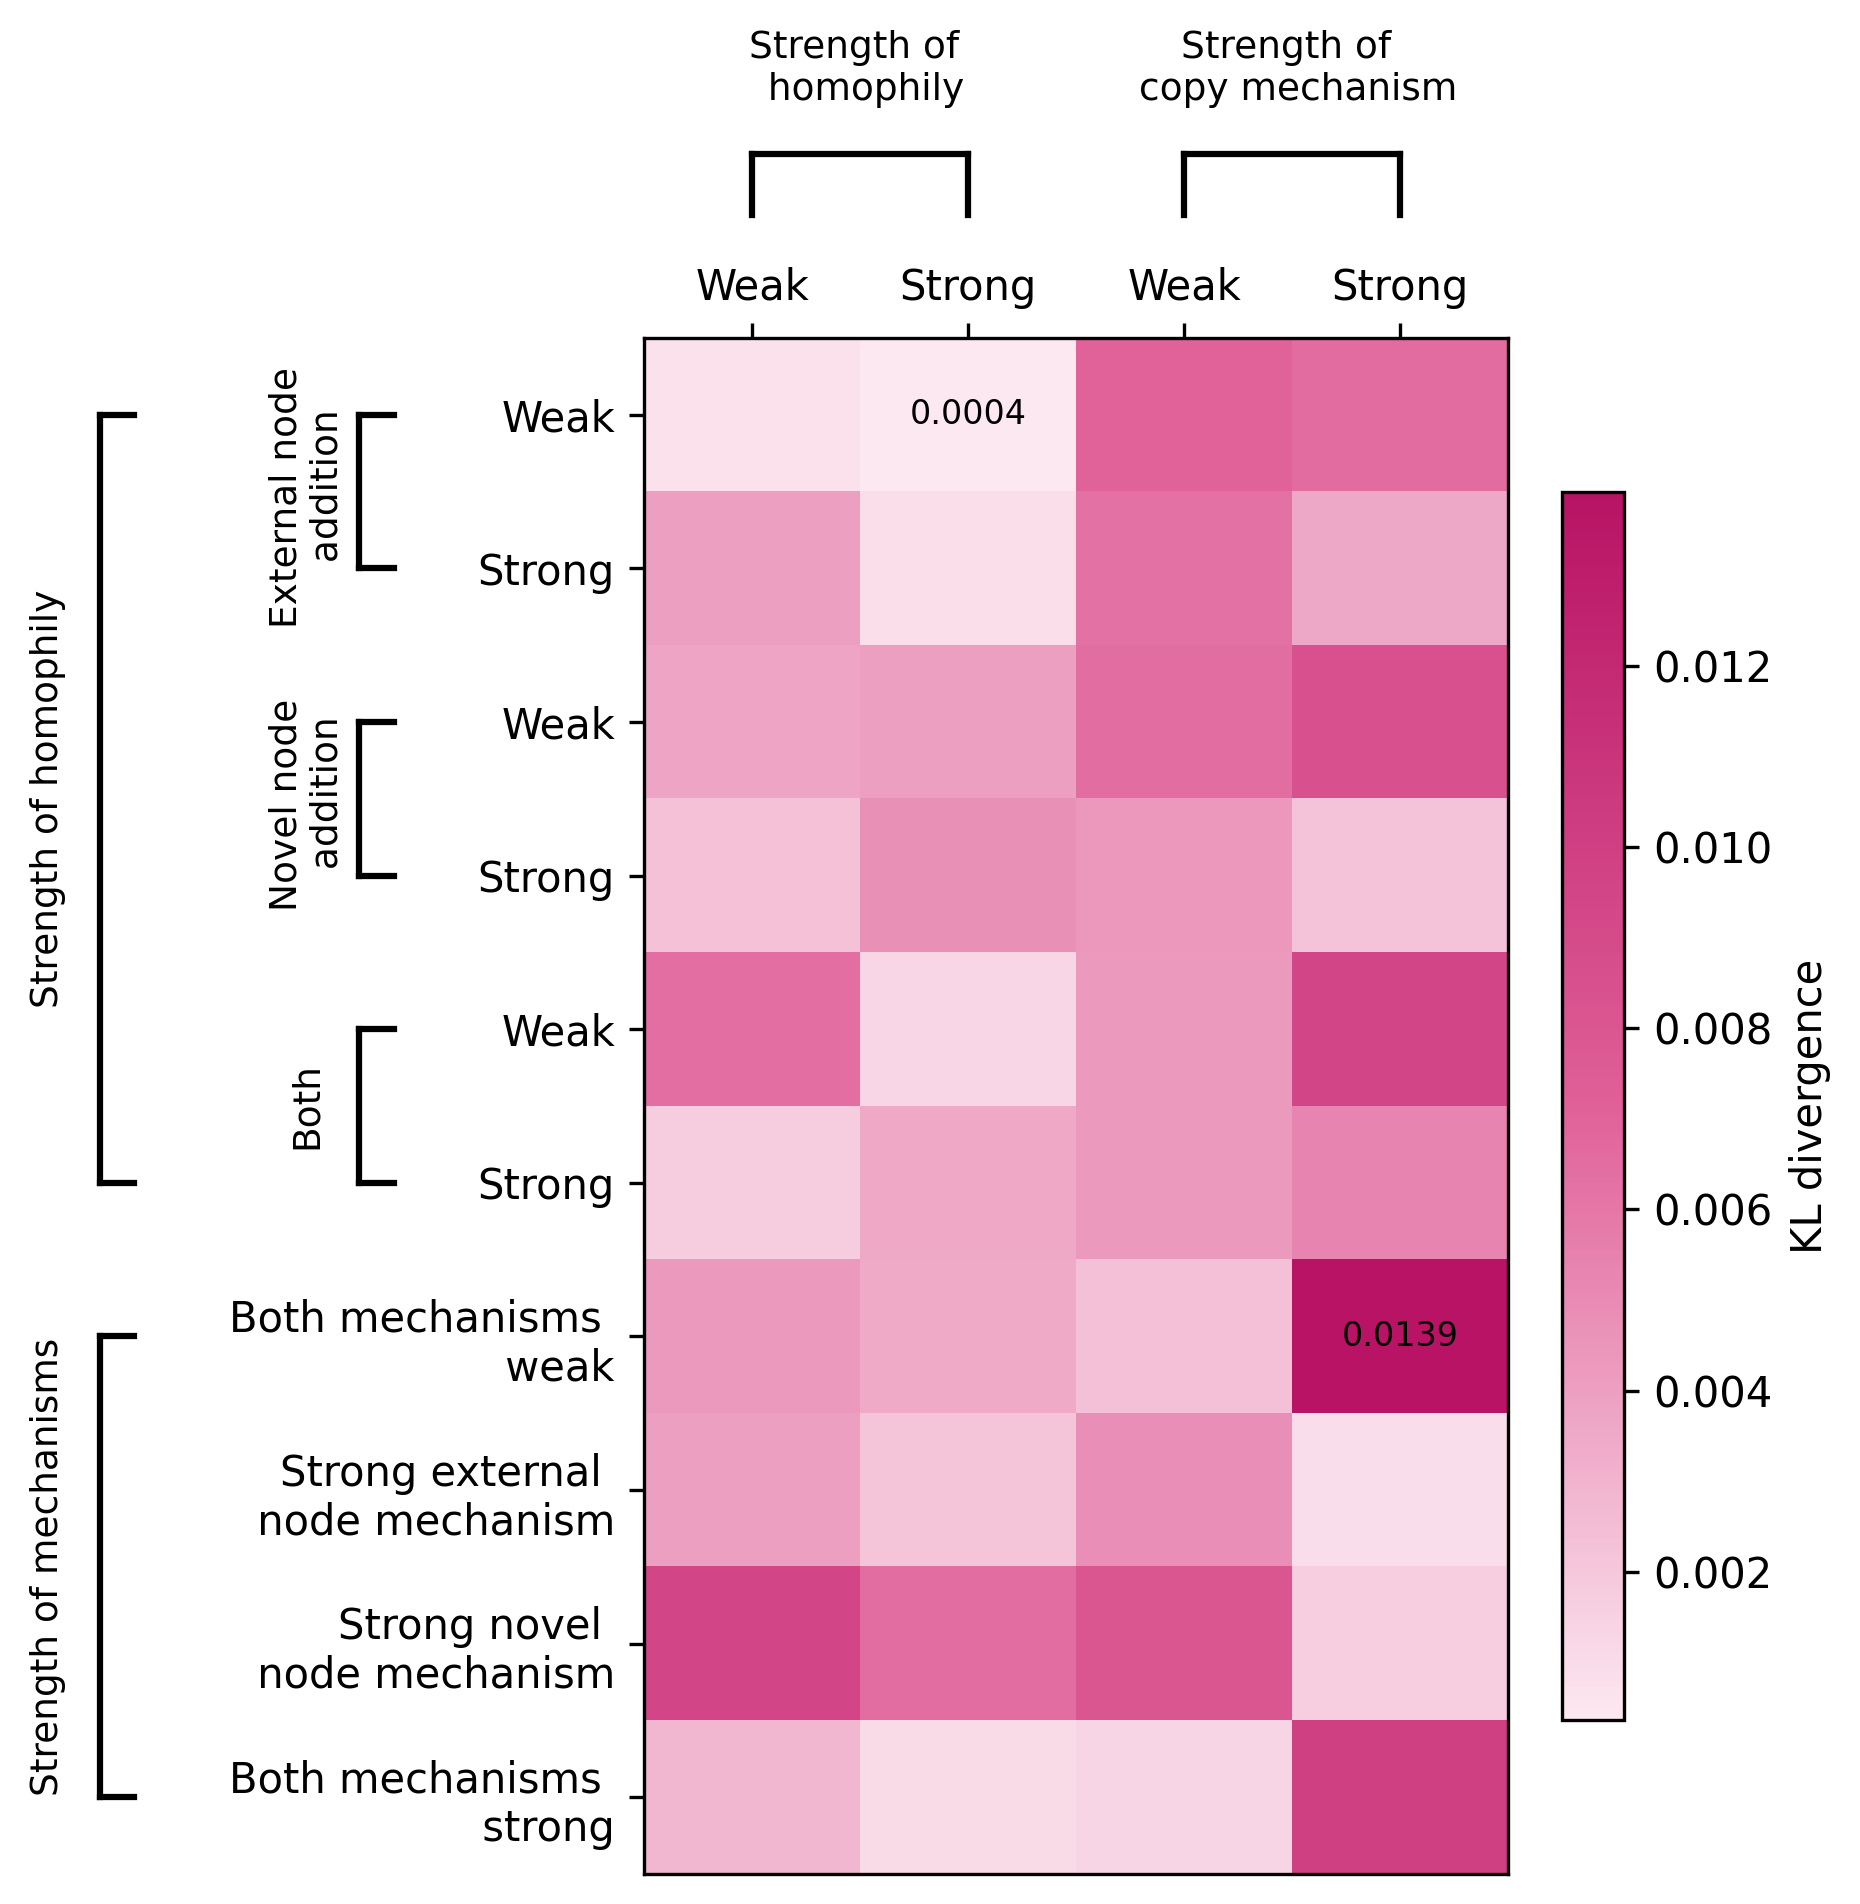
\includegraphics[width=\textwidth]{../fig/sem_convergence_heatmap.png}
    \caption{
        Performance of SEM on synthetic hypergraphs. 
        Each entry in the heatmap (panel (a)) corresponds to a set of parameters $\paramvector$, which can be found in Appendix \ref{sec:SEM-appendix}.        
        For each set of parameters, 20 independent hypergraphs are simulated under the \model{} model for 2,000 simulation steps. 
        We then perform SEM on each.  
        We then compute the Kullback-Leibler (KL) divergence of the estimated parameters from the true ones (\cref{eq:kl-divergence}) and average the results to obtain a value in a pixel. 
        The parameter estimates over iterations of SEM are plotted for the underlying parameters which produced the lowest mean KL divergence (copy parameters in panel (b) and addition parameters in panel (c)), 
        and similarly for the parameters that produced the highest mean KL divergence in panels (d) and (e).
        \DIFaddbeginFL \phil{Violet, I think we need you to more closely tie the table to the specific tables in Appendix F. Which parts of plot for which tables?}
    \DIFaddendFL }
    \label{fig:synthetic_sem}
\end{figure*}

\Cref{fig:synthetic_sem} illustrates the behavior of SEM in recovering parameters from synthetic hypergraphs generated by the \model{} model.
Each synthetic hypergraph is generated \DIFdelbegin \DIFdel{using our model and }\DIFdelend \DIFaddbegin \DIFadd{by simulating }\model{} \DIFadd{with }\DIFaddend a known parameter vector $\paramvector$.
We perform\DIFdelbegin \DIFdel{ed}\DIFdelend  SEM on a set of hypergraphs that were generated with varying \DIFdelbegin \DIFdel{amounts }\DIFdelend \DIFaddbegin \DIFadd{strengths }\DIFaddend of homophily across each of the three growth mechanisms: the edge copy step, the extant node addition step, and the novel node addition step.
We also \DIFdelbegin \DIFdel{varied }\DIFdelend \DIFaddbegin \DIFadd{vary }\DIFaddend the expected number of nodes added to $e$ in each of these steps.
To measure the success of a parameter recovery, we compute the Kullback-Leibler (KL) divergence between the true and estimated distributions described by each of the six parameters, and add the results. 
Using standard results, our measure of error \DIFdelbegin \DIFdel{then becomes
}\DIFdelend \DIFaddbegin \DIFadd{is given by 
}\DIFaddend \begin{align}
    \DIFdelbegin \DIFdel{D}%DIFDELCMD < [%%%
\DIFdel{p_{\paramvector} || }%DIFDELCMD < \hat{p}%%%
\DIFdel{_{\paramvector{}}}%DIFDELCMD < ] %%%
\DIFdelend \DIFaddbegin \DIFadd{\delta_{\mathrm{KL}} }\DIFaddend &= \phantom{+}\sum_{* \in \{+, -\}} c_*\left( \copyrate_{*} \log \frac{\copyrate_{*}}{\hat{\copyrate}_{*}} +  (1 - \copyrate_{*}) \log \frac{1 - \copyrate_{*}}{1 - \hat{\copyrate}_{*}} \right) \nonumber\\ 
    &\phantom{=} + \sum_{* \in \{+, -\}} \left( \extantrate_{*} \log \frac{\extantrate_{*}}{\hat{\extantrate}_{*}} - \extantrate_* + \hat{\extantrate}_{*} \right) \label{eq:kl-divergence} \\ 
    &\phantom{=} + \sum_{* \in \{+, -\}} \left( \novelrate_{*} \log \frac{\novelrate_{*}}{\hat{\novelrate}_{*}} - \novelrate_* + \hat{\novelrate}_{*} \right)\;, \nonumber
\end{align}
where $c$ is a factor describing, in expectation, how many nodes of each label are selected in the copy step. 
For this analysis, we set $c_* = 1$ for both labels.

As seen in \Cref{fig:synthetic_sem}, the quality of the learned parameter estimates depends on the seeded parameter vector. 
We observe especially low estimation errors when the seeded parameters reflect high copy rates $\copyrate_{*}$ and \DIFaddbegin \DIFadd{strong }\DIFaddend homophily as reflected in the differences $\same{\extantrate} - \opp{\extantrate}$ and $\same{\novelrate} - \opp{\novelrate}$; a typical SEM run for these parameter settings is shown in the top row on the right of \Cref{fig:synthetic_sem}.
That said, even in the least successful cases for estimation with high KL divergence, the learned estimates are still visually close to the true values, illustrated in the bottom row on the right of \Cref{fig:synthetic_sem}. 

\subsection{Parameter Estimation on Empirical Data} \label{sec:sem-empirical}

We also used our method to infer parameters for six standard empirical hypergraph datasets described in \Cref{tab:datasets}. 
Although many labeled hypergraph data sets are now available for community detection, relatively few have natively binary node labels. 
The \texttt{senate-bills} and \texttt{house-bills} datasets \cite{fowler2006connecting,fowler2006legislative} are hypergraphs of cosponsorships of bills in the U.S. Senate and House of Representatives, respectively, with node labels corresponding to the political party of each legislator; we use the version of these data sets used in \cite{chodrowGenerativeHypergraphClustering2021}.
The \texttt{high-school} and \texttt{primary-school} datasets \cite{gemmetto2014mitigation,stehle2011high,mastrandrea2015contact} are \DIFdelbegin \DIFdel{parsed into }\DIFdelend hypergraphs of social interactions between students in a high school and primary school, respectively, with node labels corresponding to the gender of each student; these data sets were collected through the SocioPatterns project.
\DIFdelbegin \DIFdel{Due to the high temporal resolution of these data }\DIFdelend \DIFaddbegin \DIFadd{In these data sets}\DIFaddend , we consider a sequence of interactions to correspond to a single hyperedge if those interactions are identical \DIFaddbegin \DIFadd{as sets }\DIFaddend and temporally contiguous. 
Finally, we considered a \texttt{coauthorship} data set \cite{agarwal2016women} which contains publishing records for 81 computer science conferences from 2000 to 2015, with a binary gender label for each author.
\frannie{Are the gender labels for coauthorship inferred?}
\DIFaddbegin \phil{Punting to Violet on this one.}
\DIFaddend 

\begin{table*}
    \caption{Data sets used in this paper. We show the number of nodes $n$, edges $m$, average degree $\langle d \rangle$, and average edge size $\langle k \rangle$ for each dataset.
    \DIFaddbeginFL \DIFaddFL{All data sets are used for parameter estimation. Only }\texttt{\DIFaddFL{senate-bills}}\DIFaddFL{, }\texttt{\DIFaddFL{high-school}}\DIFaddFL{, and }\texttt{\DIFaddFL{primary-school}} \DIFaddFL{are used in community detection experiments.}\DIFaddendFL }\label{tab:datasets}
        \begin{tabular}{lrrrrrrr}
        % \toprule
        & $n$ & $m$ & $\langle d \rangle$ & $\langle k \rangle$ & Nodes are & Edges are & Labels represent\\
        \midrule
        \texttt{senate-bills} \cite{fowler2006connecting,fowler2006legislative,chodrowGenerativeHypergraphClustering2021} & 294 & 29,157 & 789.6 & 8.0 & Senators & Cosponsored bills & Political party\\
        \texttt{house-bills} \cite{fowler2006connecting,fowler2006legislative,chodrowGenerativeHypergraphClustering2021} &  1,494 & 60,987 & 835.8 & 20.5 & Congresspeople & Cosponsored bills & Political party  \\
        \texttt{high-school} \cite{gemmetto2014mitigation,stehle2011high} & 320 & 60,544 & 484.6 & 2.6 & Students & Social interactions & Gender  \\
        \texttt{primary-school} \cite{mastrandrea2015contact} & 227 & 44,626 & 590.7 & 3.0 & Students & Social interactions & Gender \\
        \texttt{enron-emails} \cite{klimt2004enron}  & 14,901 & 83,372 & 18.5 & 3.3 & Email addresses & Email threads & Fringe vs. core \\
        \texttt{coauthorship} \cite{agarwal2016women} & 105,256 & 142,834 & 3.4 & 2.5 & Authors & Papers & Gender \\
        \bottomrule
        \end{tabular}
\end{table*}
\Cref{fig:empirical_sem} shows our parameter estimates for each of the empirical data sets under the \model{} model. 
In each panel, we plot the same-label and opposite-label parameter estimates on opposing axes. 
Some data sets, like the gendered primary school contact network, appear on or near the line of equality in all three panels, suggesting that \DIFdelbegin \DIFdel{there is little selection in network evolution }\DIFdelend \DIFaddbegin \DIFadd{homophily }\DIFaddend with respect to the \DIFdelbegin \DIFdel{chosen binary labels }\DIFdelend \DIFaddbegin \DIFadd{given binary labels is not a major driver of network evolution}\DIFaddend . 
The coauthorship data, meanwhile, falls on the line of equality for the edge copy and extant node addition mechanisms, but there is a difference in the novel node addition parameters: $\same{\hat{\novelrate}} > \opp{\hat{\novelrate}}$.
Our model presents a simplified picture of the process of collaboration formation as being initiated by a focal individual scientist, who then recruits from a previous collaboration, from other published scientists in the field, and from an unobserved pool of novices who have never published before. 
Our findings suggest that of these mechanisms, only the latter (the recruitment of novices) displays substantial gender homophily, with novices who share the gender of the focal scientist more likely to be recruited to the collaboration. 
This effect may be partially due to gender homophily between PhD students and their advisors, a known phenomenon in several scientific areas \cite{schwartz2022impact}. 

The \texttt{senate-bills} dataset appears to have \DIFdelbegin \DIFdel{slight }\DIFdelend \DIFaddbegin \DIFadd{weak }\DIFaddend homophily in the estimates of the edge copy and extant node addition parameters.
Because new senators are elected far less frequently than bills are cosponsored, the novel node addition parameters are both nearly 0. 
The analogous \texttt{house-bills} data set has edge copy parameter estimates which are relatively similar to those of \texttt{senate-bills}, but which suggest a small tendency towards heterophily rather than homophily in edge-copying. 
The slight heterophily in the copy step of \texttt{house-bills} may be related to reciprocity in bipartisan cosponsorship, a phenomenon that has been observed in U.S. legislative bodies \cite{harbridge2023bipartisan,dobson2026selective}.
We illustrate the connection between reciprocity and edge copy parameters through the following example.
Consider some bill $\newedge$, where $\focalnode$ is a cosponsor of both bill $\newedge$ and bill $\seededge$.
If $\focalnode$ is a Democrat, for instance, and the primary sponsor of $\seededge$ is a Republican, then $\focalnode$ was a ``bipartisan'' cosponsor of $\seededge$.
The reciprocity of bipartisan cosponsorship suggests that the Republican cosponsors of $\seededge$ may also cosponsor $\newedge$ to \DIFdelbegin \DIFdel{``}\DIFdelend return the favor.
\DIFdelbegin \DIFdel{''
}\DIFdelend However, the other Democratic cosponsors of $\seededge$ are not indebted in the same way to $\focalnode$, \DIFdelbegin \DIFdel{perhaps }\DIFdelend \DIFaddbegin \DIFadd{possibly }\DIFaddend making them less likely to cosponsor $\newedge.$
The mechanisms of and motivations for bipartisan reciprocity vary between the House and the Senate \cite{dobson2026selective}, which may in part explain why we observe heterophily in edge copying for \texttt{house-bills} but not \texttt{senate-bills}.
\DIFaddbegin \DIFadd{Further investigation of the relationship between reciprocity and edge copying in legislative cosponsorship is an interesting direction for future work.
}\DIFaddend 


The novel node estimates are also very small. 
The \DIFdelbegin \DIFdel{biggest }\DIFdelend \DIFaddbegin \DIFadd{largest }\DIFaddend difference in our estimates for these two systems is in the extant node addition parameter estimates; the \texttt{house-bills} data set has estimates $\same{\hat{\extantrate}}$ and $\opp{\hat{\extantrate}}$ which are each roughly three times larger than their values in the \texttt{senate-bills} data set.
These estimates suggest the operation of similar levels of party homophily in the cosponsorship of bills \DIFaddbegin \DIFadd{via extant node addition}\DIFaddend , but with proportionally more of the legislators sponsoring a bill originating in the House having been previously uninvolved with a previous ``seeding'' bill.  
These estimates reflect the higher mean edge size of \texttt{house-bills}, where a bill is co-sponsored by a mean of over 20 congresspersons, as opposed to the mean of 8 in \texttt{senate-bills}. 
% That is, a bill in the House of Representatives has on average more cosponsors than a bill in the Senate, and since only about half of $\seededge$ is copied to $\newedge$, and $\opp{\novelrate}$ and $\same{\novelrate}$ are close to zero, the extant node parameters will grow proportionally to the mean edge size.

    
The emails hypergraph falls in the heterophilic region of the edge copy panel.
This is a feature of the sampling strategy.
The Enron dataset contains the email data from 145 users associated with the Enron Corporation.
These users are the ``core'' nodes of the hypergraph.
Any users who were included in emails with core users, but whose complete email data was not sampled, are referred to as ``fringe'' nodes.
Each hyperedge represents an email between a set of nodes, or users.
Therefore, each hyperedge must contain at least one core node.
\DIFdelbegin \DIFdel{And since }\DIFdelend \DIFaddbegin \DIFadd{Since }\DIFaddend 73\% of edges in the hypergraph have size 2, and less than one percent of the nodes in the hypergraph are core nodes, \DIFdelbegin \DIFdel{any given edge likely contains one core node and one fringe node.
In fact, }\DIFdelend \DIFaddbegin \DIFadd{most edges (}\DIFaddend 67\DIFdelbegin \DIFdel{\% of edges in the Enron data match exactly this description}\DIFdelend \DIFaddbegin \DIFadd{\%) join a core node to a fringe node, generating disassortativity with respect to these labels}\DIFaddend .  
The high magnitude of the copy parameters, particularly $\copyrate_-$, is a result of the nature of email — rarely does an email interaction between a group of users occur only once.
Often, an email is precipitated by an existing conversation between that set of users, making the edge copy mechanism well suited for modeling email network growth.


\begin{figure}[t]
    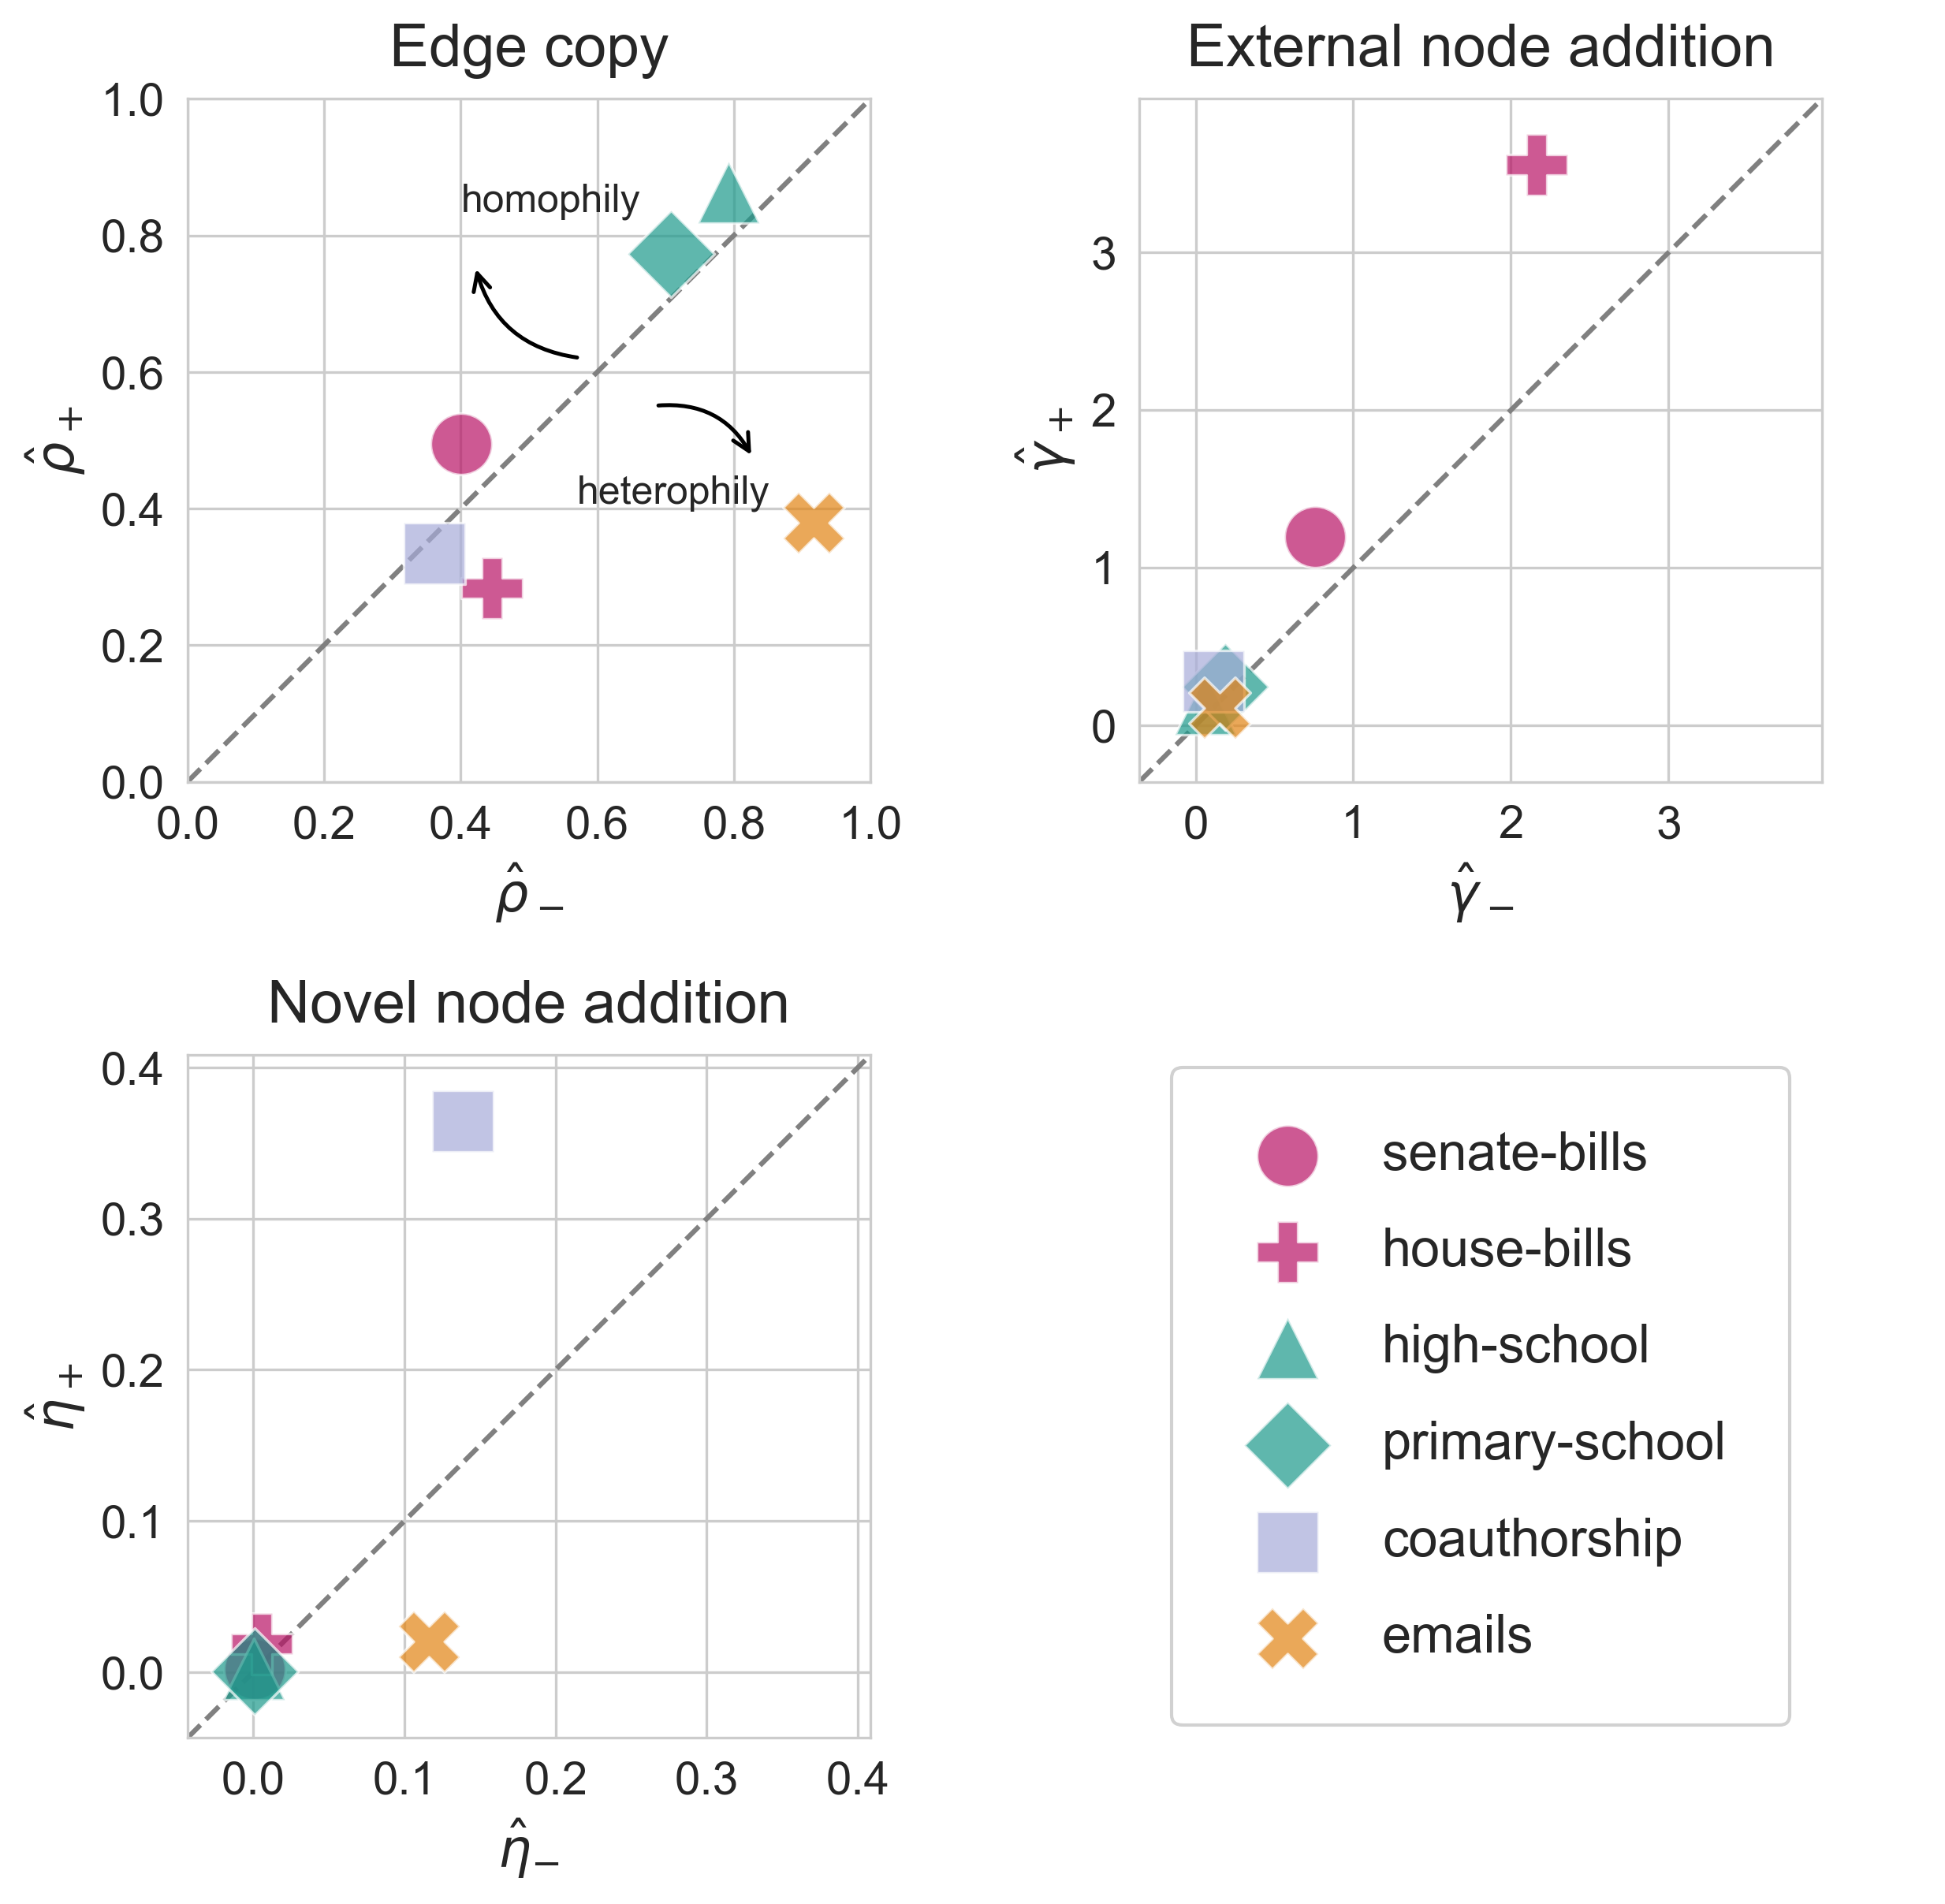
\includegraphics[width=0.5\textwidth]{../fig/empirical_sem.png}
    \caption{
        Model parameters inferred via SEM for six empirical higher-order networks.
        The line of equality is shown as a guide for the eye.
        }
     \label{fig:empirical_sem}
\end{figure}






\subsection{Community Detection via Simulated Annealing}


\begin{figure}
    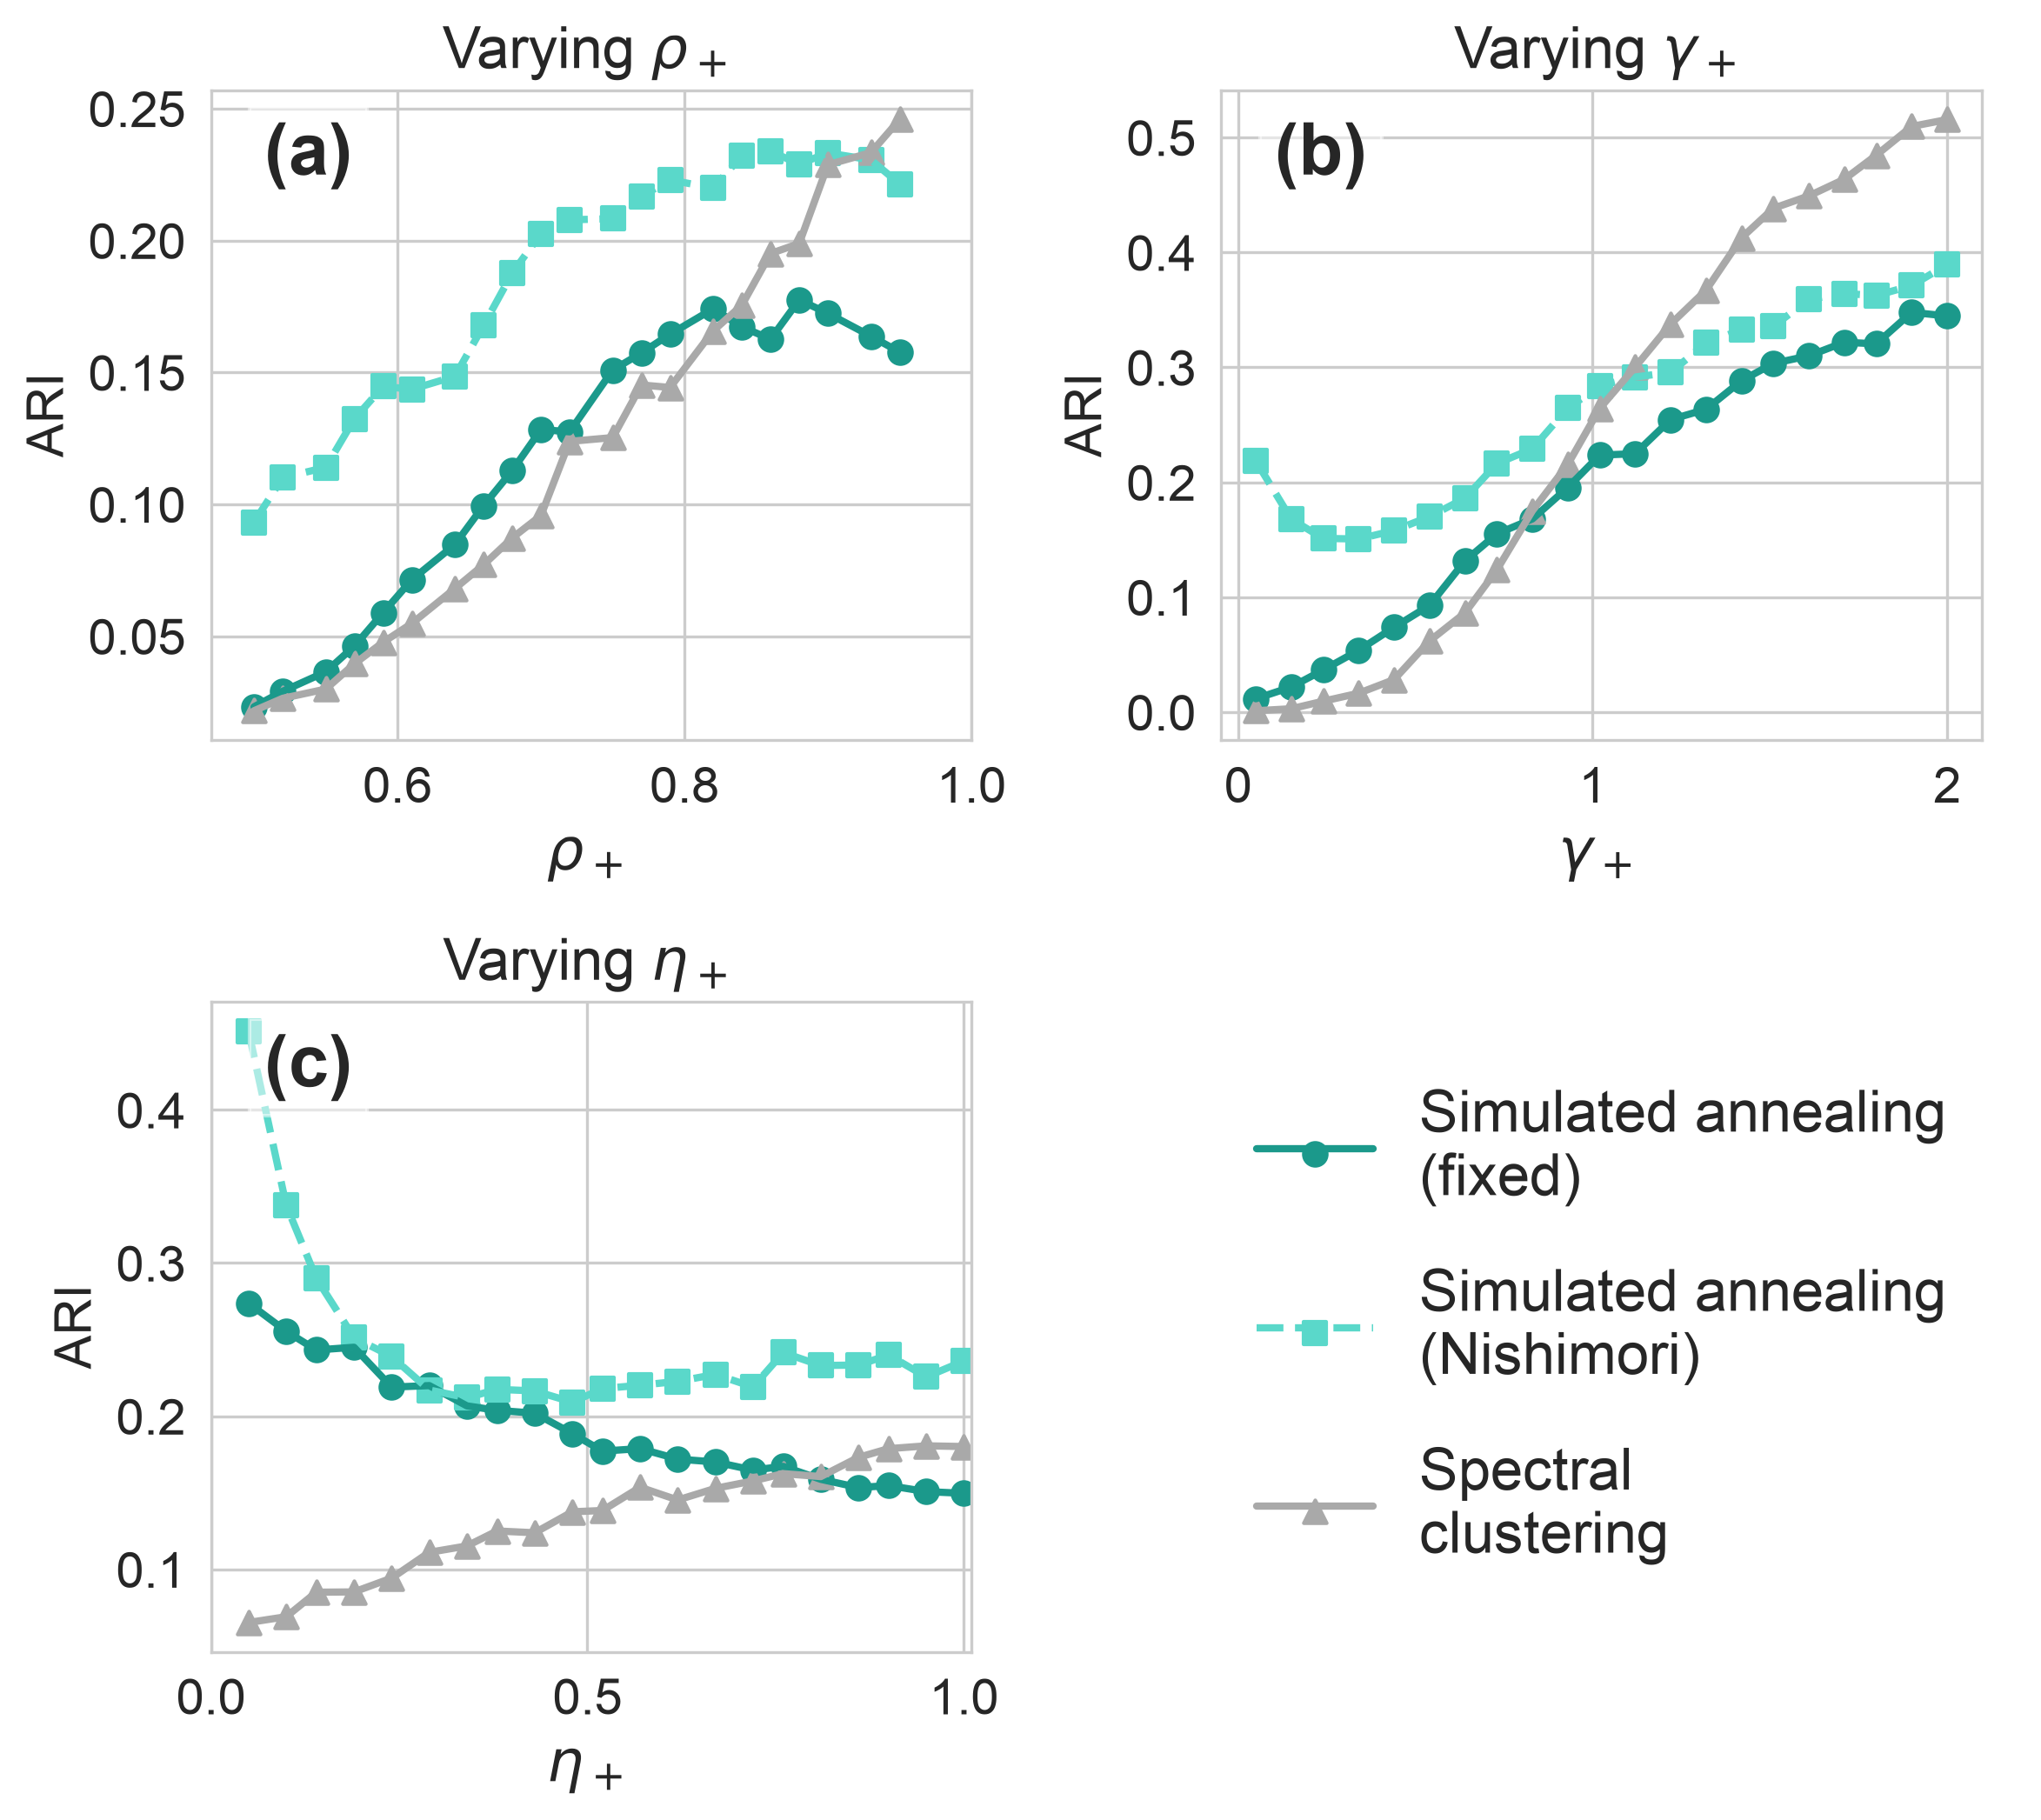
\includegraphics[width=\columnwidth]{../fig/community-synthetic-data-viz-line.png}
    \caption{
        Comparison of community detection methods on synthetic data. 
        We compare our simulated annealing algorithm under the Nishimori condition and with a fixed parameter vector $\paramvector' = \thetaguess$ against a baseline of Laplacian spectral clustering on the weighted clique projection of the hypergraph. 
        The ``default'' parameter vector used in synthetic hypergraph generation is $\paramvector = (\same{\copyrate}, \opp{\copyrate}, \same{\extantrate}, \opp{\extantrate}, \same{\novelrate}, \opp{\novelrate}) = (\synthfixedetaplus,\synthfixedetaminus, \synthfixedlambdaplus, \synthfixedlambdaminus,\synthfixedgammaplus, \synthfixedgammaminus)$. 
        In each of the three panels (a-c), a single one of these parameters is varied while the others are held fixed at their default values. 
        Each point gives the mean ARI over 500 independent model simulations, each of which was simulated for 200 timesteps. 
    } \label{fig:community-synthetic}
\end{figure}

We evaluate our simulated annealing algorithm on a range of small synthetic data sets under two conditions, shown in \Cref{fig:community-synthetic}. 
Under the Nishimori condition \cite{decelle2011asymptotic}, we generate a synthetic hypergraph according to a parameter vector $\paramvector$ and then attempt to learn $\vz$ via simulated annealing using the same parameter vector $\paramvector$. 
Under the ``fixed'' condition, which simulates a more realistic data analysis scenario, we always use the same parameter vector $\paramvector'$ to learn $\vz$ via simulated annealing \DIFdelbegin \DIFdel{, }\DIFdelend regardless of the true parameter vector $\paramvector$ used to generate the synthetic data. 
In this condition, we use a default value of $\paramvector' = \thetaguess$. 
We compare these methods against each other and against a baseline of Laplacian spectral clustering \cite{luxburg2007tutorial} applied to the weighted clique projection of the hypergraph. 
We assess the effectiveness of these techniques and our method with a measure of clustering effectiveness, the adjusted Rand index (ARI) \cite{hubert1985comparing}.
In each panel of \Cref{fig:community-synthetic}, we show the performance of each of these models as a single entry of $\paramvector$ is varied while the others are held fixed. 
Unsurprisingly, simulated annealing under the Nishimori condition outperforms simulated annealing under the fixed condition. 
For \DIFdelbegin \DIFdel{high levels of }\DIFdelend \DIFaddbegin \DIFadd{strong }\DIFaddend homophily (larger values of the varied parameter), simulated annealing under the Nishimori condition can nevertheless be outperformed by Laplacian spectral clustering. 
Notably, however, there are regions of parameter space, especially those with \DIFdelbegin \DIFdel{low levels of }\DIFdelend \DIFaddbegin \DIFadd{weak }\DIFaddend homophily (smaller values of the varied parameter), in which both simulated annealing under the fixed condition and under the Nishimori condition outperform Laplacian spectral clustering. 
This result is in some sense unsurprising, since we perform our experiment on synthetic samples drawn directly from the \model{} model.
\DIFdelbegin \DIFdel{These experiments do suggest , however, }\DIFdelend \DIFaddbegin \DIFadd{Nevertheless, these experiments suggest }\DIFaddend that there exist classes of hypergraphs in which community structure can be more reliably detected via likelihood maximization under \model{} than by at least this standard graph method. 

\DIFdelbegin \DIFdel{We can see this phenomenon in experiments }\DIFdelend \DIFaddbegin \DIFadd{Indeed, we observe relatively favorable performance of the }\model{} \DIFadd{model }\DIFaddend on empirical data as well. 
We evaluate our simulated annealing algorithm on a subset of our empirical data sets: \texttt{senate-bills}, \texttt{primary-school}, and \texttt{high-school}; the poor scaling of simulated annealing with the number of nodes $n$ made it computationally prohibitive to run on the larger \texttt{house-bills}, \texttt{enron-emails}, and \texttt{coauthorship} data sets.
We use the class membership of the students in \texttt{primary-school} and \texttt{high-school} as the ground truth labels in this section instead of gender because community structure has been previously detected with these labels \cite{chodrowGenerativeHypergraphClustering2021}.  
Since in data analysis contexts the labels $\vz$ (and therefore parameter estimates $\hat{\paramvector}$) are not available, we instead use a single, fixed parameter vector for each of these three experiments: \DIFdelbegin \DIFdel{$\hat{\paramvector} = (0.9, 0.1, 1.0, 0.25, 0.001, 0.001)$.
}\DIFdelend \DIFaddbegin \DIFadd{$\hat{\paramvector} = (0.90, 0.10, 1.00, 0.25, 0.00, 0.00)$.
The zero values for the novel node addition parameters reflect a choice of algorithmic convenience. 
}\DIFaddend All of these datasets are appropriately modeled with very small values of $\same{\novelrate}$ and $\opp{\novelrate}$ under our model due to their large number of edges compared to the small number of nodes.  
\DIFdelbegin \DIFdel{Since in these three data sets many of the nodes exist in the system before data collection, for the purposes of community detection, we ignore the novel node addition step, assuming instead }\DIFdelend \DIFaddbegin \DIFadd{To simplify computation, we instead simply assume }\DIFaddend that all nodes \DIFdelbegin \DIFdel{are present }\DIFdelend \DIFaddbegin \DIFadd{exist }\DIFaddend in the system \DIFdelbegin \DIFdel{and eligible to be added via the extant node addition step. 
}\DIFdelend \DIFaddbegin \DIFadd{at all times, even if they have not yet participated in an edge. 
}

\DIFaddend We compare \model{} simulated annealing against several competitors. 
The all-or-nothing hypergraph modularity of \cite{chodrowGenerativeHypergraphClustering2021} does not allow the user to specify a desired number of clusters, but because it returns a binary partition on \texttt{senate-bills}, we can compare directly on this data set. 
Belief-propagation nonbacktracking spectral clustering \cite{chodrowNonbacktrackingSpectralClustering2023} allows the user to specify the number of clusters, and the authors report results for binary clustering. 
We therefore compare our method against the reported results from these two \DIFdelbegin \DIFdel{articles}\DIFdelend \DIFaddbegin \DIFadd{prior works}\DIFaddend .\footnote{The authors of \cite{chodrowNonbacktrackingSpectralClustering2023} did not perform the data filtering on \texttt{high-school} and \texttt{primary-school} described in \Cref{sec:sem-empirical}, so our direct comparison with their results should be interpreted with some caution.}
Notably, both hypergraph modularity maximization and nonbacktracking spectral clustering are based on generative models which assume conditional edge independence, the assumption relaxed by \model{}.
We also include as comparisons two dyadic methods, implemented on the weighted clique projection of the hypergraph, that allow the user to specify the number of clusters: Laplacian spectral clustering \cite{luxburg2007tutorial} and greedy modularity maximization \cite{clauset2004finding}\DIFaddbegin \DIFadd{, both of which also have connections to generative models that assume conditional (dyadic) edge independence \mbox{%DIFAUXCMD
\cite{newman2016equivalence,lei2015consistency}}\hskip0pt%DIFAUXCMD
}\DIFaddend .

\begin{figure}
    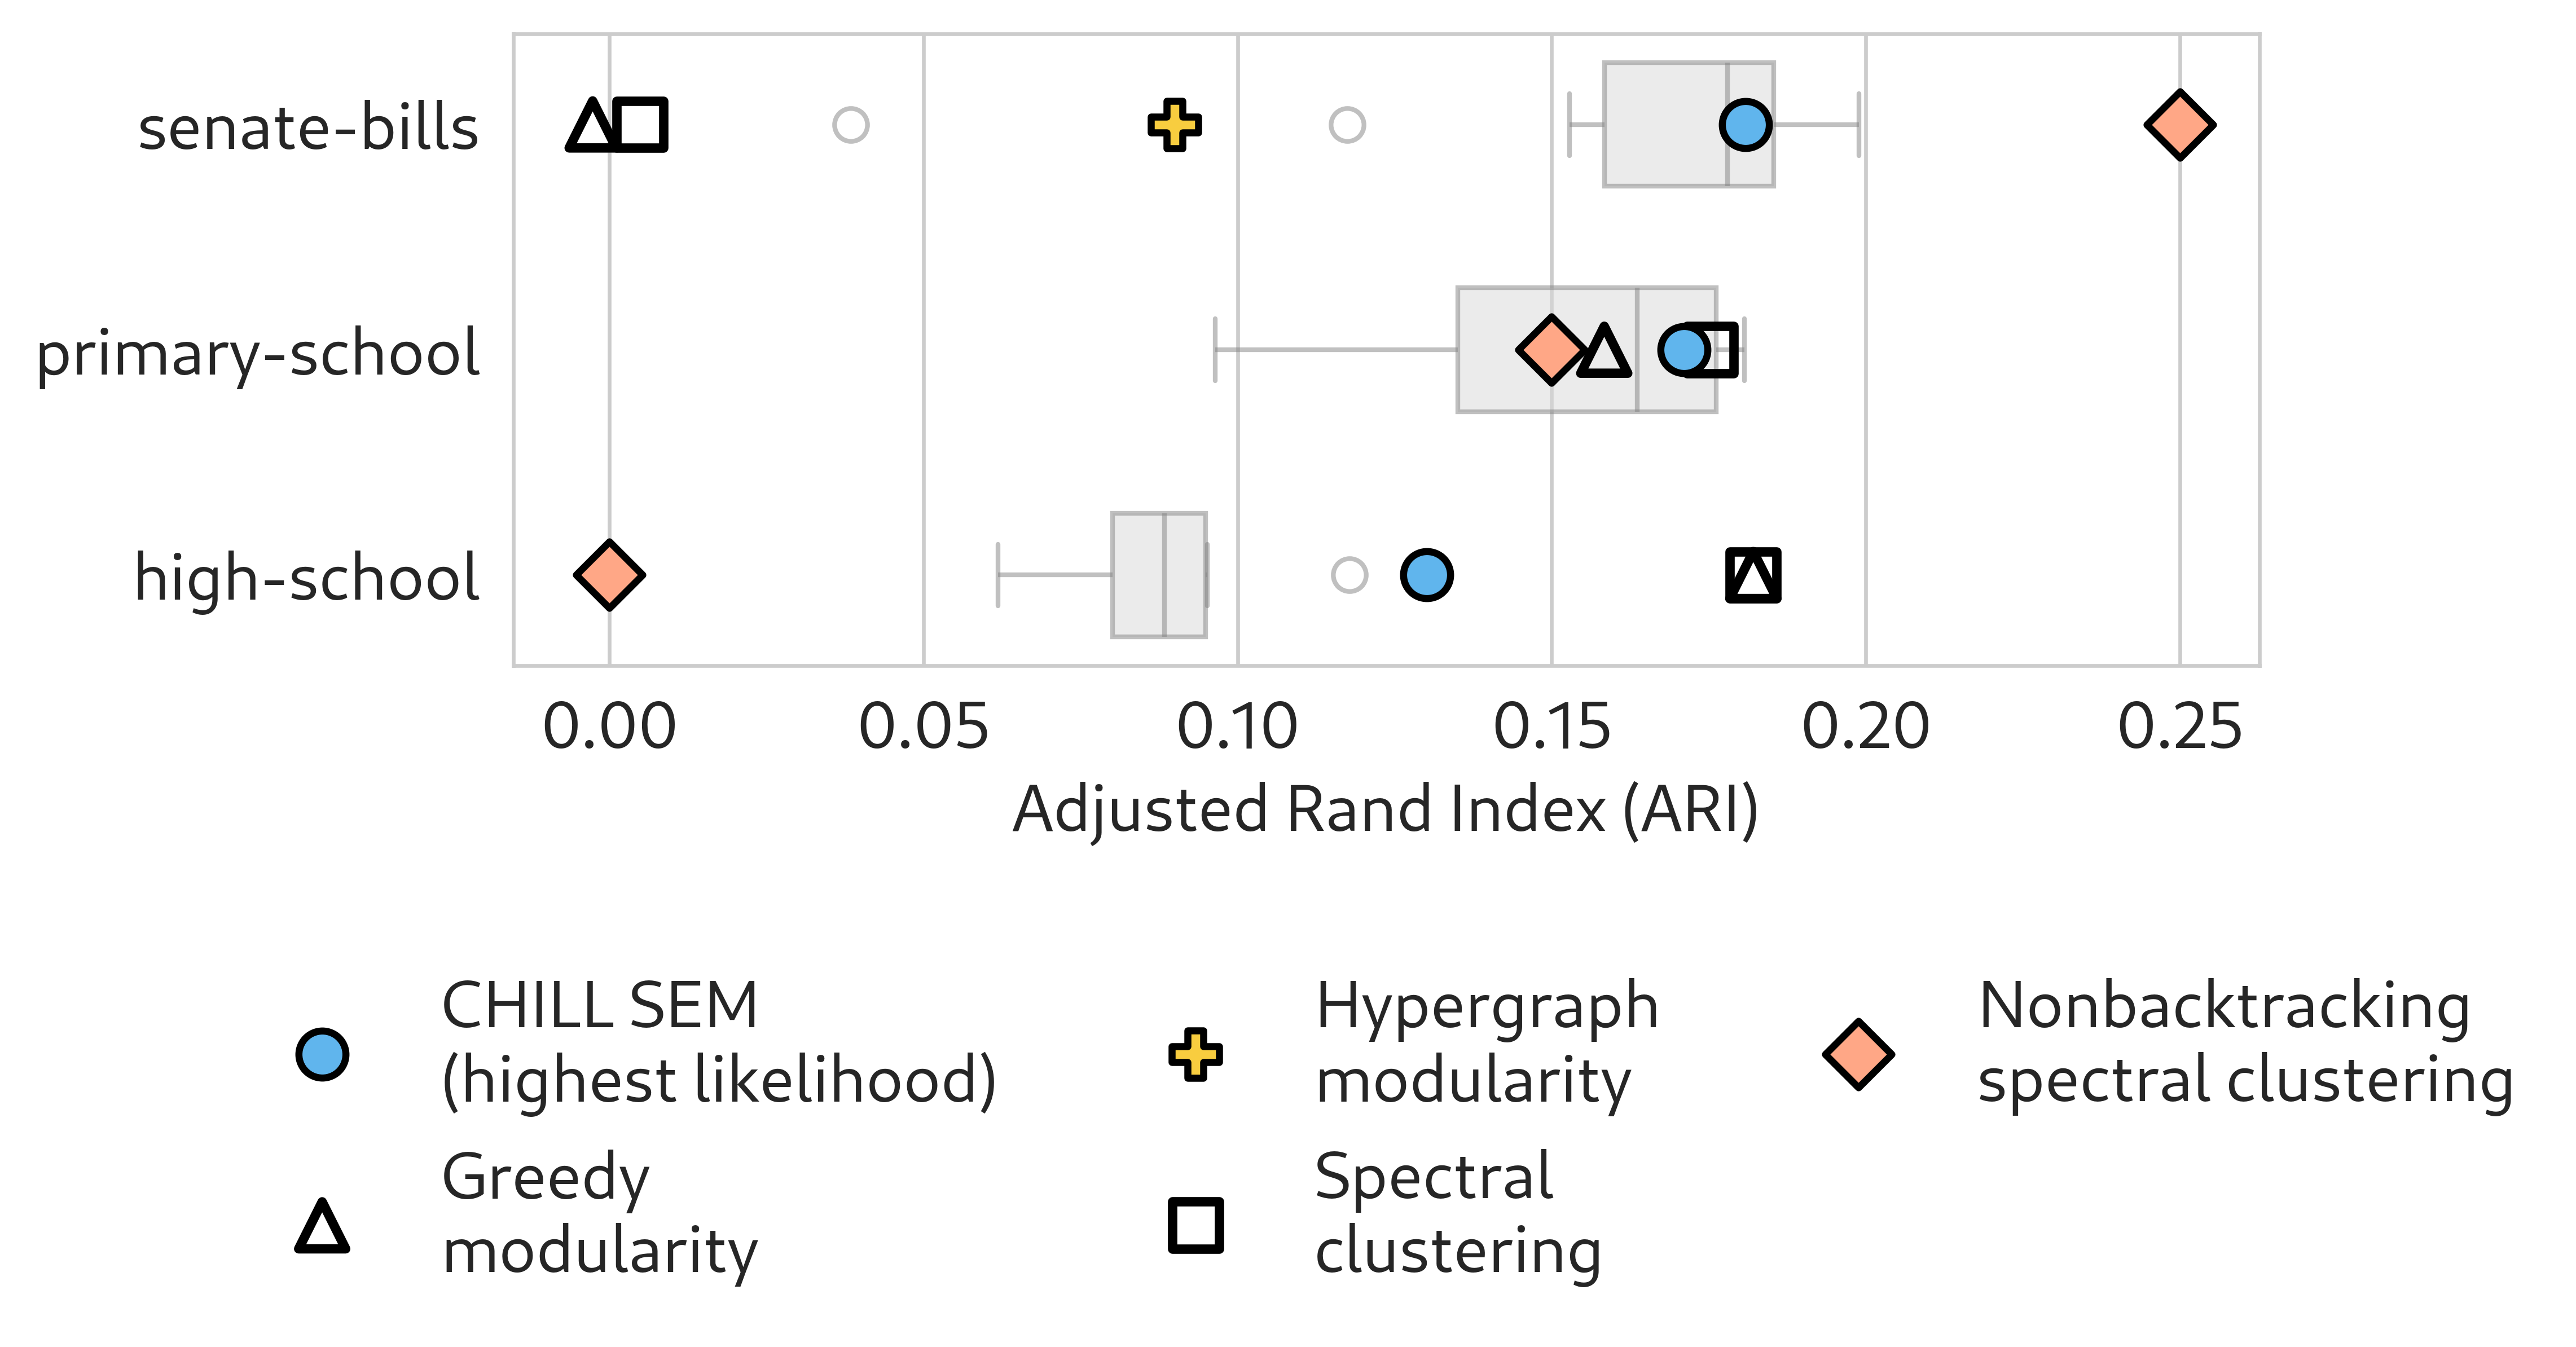
\includegraphics[width=\columnwidth]{../fig/community_detection_boxplot.png}
    \caption{Community detection results on three selected empirical datasets.  
    Box plots describe the distribution of the ARI of \model{} simulated annealing on the selected data set across 10 separate runs. 
    The single label set achieving the highest likelihood under simulated annealing is highlighted. 
    We compare these results with the ARI of the labels generated via several comparisons: hypergraph modularity \cite{chodrowGenerativeHypergraphClustering2021} (only for \texttt{senate-bills}), belief-propagation nonbacktracking spectral clustering \cite{chodrowNonbacktrackingSpectralClustering2023}, greedy dyadic modularity maximization \cite{clauset2004finding}, and dyadic Laplacian spectral clustering \cite{luxburg2007tutorial}; the latter two dyadic methods are denoted by hollow markers.  
    Values for hypergraph modularity maximization and nonbacktracking spectral clustering are reported in \cite{chodrowGenerativeHypergraphClustering2021} and \cite{chodrowNonbacktrackingSpectralClustering2023}, respectively.
    }
    \label{fig:community-empirical}
\end{figure}

In \Cref{fig:community-empirical}, we observe that \model{} simulated annealing outperforms both \DIFdelbegin \DIFdel{greedy-modularity and spectral clustering on senate bills }\DIFdelend \DIFaddbegin \DIFadd{of the dyadic methods---greedy-modularity and spectral clustering---on }\texttt{\DIFadd{senate-bills}} \DIFaddend in all 10 runs in ARI.  
On \DIFdelbegin \DIFdel{the primary school dataset}\DIFdelend \DIFaddbegin \texttt{\DIFadd{primary-school}}\DIFaddend , simulated annealing performs comparably in ARI to the competitor methods, with a slightly lower average ARI compared to spectral clustering and greedy modularity's results.  
However, simulated annealing performs worse on \DIFdelbegin \DIFdel{the high school dataset }\DIFdelend \DIFaddbegin \texttt{\DIFadd{high-school}} \DIFaddend in ARI compared to its competitors.
\DIFdelbegin \DIFdel{While the computational performance of simulated annealing presents a difficulty in its application, the detectionof communities via the maximization of likelihood provides evidence that the formations of these datasets, especially senate-bills, can be simulated via our proposed model $\model$.
Further, the success of our model in comparison to spectral clustering and greedy modularity provides evidence challenging the assumption of edge independence within }\texttt{\DIFdel{senate-bills}}%DIFAUXCMD
\DIFdel{. 
This is because the baseline methods, greedy modularity and spectral clustering, are frequently justified via the stochastic block model \mbox{%DIFAUXCMD
\cite{lei2015consistency, newman2016equivalence}}\hskip0pt%DIFAUXCMD
, which relies on the assumption of edge indepenece, where our method explicitly utilizes dependent hyperedges.
}%DIFDELCMD < \frannie{Is this paragraph left over, or did you want to keep this Phil?}
%DIFDELCMD < %%%
%DIF <  \frannie{Unsure of the assumptions behind spectral clustering, tried to google but couldn't find.  If assumption of edge independence, could say something about that}
\DIFdelend \DIFaddbegin \DIFadd{The relatively consistent performance of }\model{} \DIFadd{simulated annealing across these three data sets suggests that explicitly modeling dependence between edges may provide promising future directions in community detection, motivating a need for much more efficient heuristics with which to carry out the optimization. 
}\DIFaddend 





%DIF <  \phil{Good idea to look on this. Spectral clustering is not a generative (probabilistic model-based) method, but many of its standard justifications do rely on stochastic block models which have the independence assumption. The best citation is probably this one: \cite{lei2015consistency}}. 
\DIFdelbegin %DIFDELCMD < 

%DIFDELCMD < %%%
\DIFdelend % \begin{figure*}
%     \includegraphics[width=\textwidth]{../fig/community-synthetic-data-viz-main.png}
%     \caption{
%         Community detection results on synthetic data.
%         Each pixel represents \synthrepetitions{} independent hypergraphs generated from our model with \synthtimesteps{} timesteps. 
%         In each heatmap, we vary $\same{\copyrate{}}$ and $\opp{\copyrate{}}$, holding $(\same{\extantrate{}}, \opp{\extantrate{}}, \same{\novelrate{}}, \opp{\novelrate{}}) =
%         (\synthfixedlambdaplus, \synthfixedlambdaminus, \synthfixedgammaplus, \synthfixedgammaminus)$. 
%     } \label{fig:community-synthetic}
% \end{figure*}


\section{Discussion}

    We have proposed \Model{} (\model{}), a generative model for the formation of binary-labeled hypergraphs in which edges form as noisy copies of previous edges \DIFdelbegin \DIFdel{, combined with the addition of }\DIFdelend \DIFaddbegin \DIFadd{to which }\DIFaddend extant and novel nodes \DIFdelbegin \DIFdel{.
    }\DIFdelend \DIFaddbegin \DIFadd{are also added
    }\DIFaddend The copying, extant, and novel node addition steps are all tuned by node labels and parameters which control the strength of homophily \DIFdelbegin \DIFdel{or heterophily }\DIFdelend in each of these steps.
    We have demonstrated efficient parameter inference in the \model{} model via stochastic expectation maximization (SEM). 
    We have also demonstrated that, in some circumstances, maximum-likelihood inference of node labels $\vz$ via simulated annealing\DIFaddbegin \DIFadd{, though computationally expensive, }\DIFaddend can outperform both dyadic and \DIFaddbegin \DIFadd{recent }\DIFaddend polyadic community detection algorithms that proceed from the assumption of conditional edge independence. 
    We interpret this latter result as proof-of-concept that explicitly modeling edge-dependence can be a useful framework for community detection in hypergraphs. 

    There are several directions for future work. 
    Most obviously, although our results show that maximum-likelihood inference in the \model{} model is promising for detecting certain kinds of community structure, the simulated annealing method we have used is \DIFdelbegin \DIFdel{impractically expensive }\DIFdelend \DIFaddbegin \DIFadd{computationally impractical }\DIFaddend on data sets of even relatively modest size. 
    Developing more efficient heuristics for maximizing the likelihood over $\vz$ will be an important direction for scalable application of the \model{} model for community detection. 
    Scalability may also imply opportunities for improved performance.
    We note, for example,  that \DIFdelbegin \DIFdel{\mbox{%DIFAUXCMD
\cite{chodrowNonbacktrackingSpectralClustering2023} }\hskip0pt%DIFAUXCMD
proposed an algorithm that obtained an }\DIFdelend \DIFaddbegin \DIFadd{belief-propagation nonbacktracking spectral clustering \mbox{%DIFAUXCMD
\cite{chodrowNonbacktrackingSpectralClustering2023} }\hskip0pt%DIFAUXCMD
achieves an }\DIFaddend ARI of approximately 0.25 on the \texttt{senate-bills} data set \DIFaddbegin \DIFadd{(\mbox{%DIFAUXCMD
\Cref{fig:community-empirical}}\hskip0pt%DIFAUXCMD
)}\DIFaddend , higher than \DIFdelbegin \DIFdel{our proposed simulated annealing method. 
    Their }\DIFdelend \DIFaddbegin \model{}\DIFadd{. 
    That }\DIFaddend algorithm requires alternating between parameter estimation and community detection phases. 
    In principle, we could attempt a similar alternating procedure \DIFdelbegin \DIFdel{in our }\DIFdelend \DIFaddbegin \DIFadd{between SEM and simulated annealing in the }\model{} \DIFaddend model, but the computational cost of simulated annealing makes this approach infeasible in practice.
    Future work to develop more efficient heuristics for community detection under our model could, in principle, enable such an alternating algorithm, with potentially improved performance. 

    There are also opportunities to extend \model{} to more realistic settings and more diverse data sets. 
    One obvious extension is to nonbinary node labels, which would enable multiway community detection algorithms. 
    Another approach is to relax the assumption that \emph{every} edge is formed through the edge-copying mechanism; one could instead allow some edges to form spontaneously without copying an earlier edge. 
    A final possible extension is to incorporate recency-bias \cite{bensonSequencesSets2018} into the copy mechanism, so that more recent edges are more likely to be copied while edges that are sufficiently old may cease to be copied at all. 
    \DIFaddbegin \DIFadd{We hope that }\model{} \DIFadd{can provide a useful jumping-off point for future work in generative modeling and algorithms for hypergraphs with edge dependence. 
}\DIFaddend 

\begin{acknowledgments}
    PSC acknowledges support from the National Science Foundation under DMS-2407058.
    Compute was provided by Middlebury College through support from the National Science Foundation under award 1827373. 
\DIFdelbegin %DIFDELCMD < 

%DIFDELCMD < %%%
\DIFdelend \end{acknowledgments}

\section*{Data Availability}

    The code used to generate the results in this paper is available at \url{https://github.com/Violet-Ross/labeled-growth}.
    Data sets are publicly available through the papers cited in \Cref{tab:datasets}.

\DIFaddbegin \section*{\DIFadd{Use of Generative Language Models}}

    \DIFadd{Generative language models were used to assist the authors in implementing the model, methods and experiments shown in this paper. 
    The authors carefully reviewed and revised all code and associated outputs. 
    The authors take full responsibility for the correctness of all methods and results presented in this paper.
    }

\DIFaddend \bibliographystyle{apsrev4-2}
\bibliography{refs} 

\appendix



    

\section{Power-Law Degree Distribution} \label{sec:degree-distribution-appendix}

    \DIFaddbegin \DIFadd{We now derive the asymptotic power law degree distribution described in \mbox{%DIFAUXCMD
\Cref{sec:degree-distribution}}\hskip0pt%DIFAUXCMD
. 
    }\DIFaddend Our derivation follows that of He et al. \cite{heEdgeCorrelationsLink2025}, which in turn is based on a derivation by Mitzenmacher \cite{mitzenmacherBriefHistoryGenerative2004}.

    At stationarity, the mean degree $\brackets{d}$ of a node satisfies 
    \begin{align}
        \brackets{d} = \frac{m}{n}\brackets{k} \;,
    \end{align}
    where \DIFdelbegin \DIFdel{$\brackets{k}$ }\DIFdelend \DIFaddbegin \DIFadd{$\brackets{k} = \brackets{k_0} + \brackets{k_1}$ }\DIFaddend is the mean edge size (computable from the stationary distribution \DIFdelbegin \DIFdel{$\jointdist \paren{k_1,k_2}$}\DIFdelend \DIFaddbegin \DIFadd{$\jointdist \paren{k_0,k_1}$}\DIFaddend ), $m$ is the number of edges, and $n$ is the number of nodes.
    In expectation, there are \DIFdelbegin \DIFdel{$\novelrate{} \triangleq \opp{\novelrate{}} + \same{\novelrate{}}$ }\DIFdelend \DIFaddbegin \DIFadd{$\novelrate{} = \opp{\novelrate{}} + \same{\novelrate{}}$ }\DIFaddend new nodes added per new edge, which means that $\frac{m}{n} \to \frac{1}{\novelrate{}}$ as $m, n \to \infty$ in expectation.
    \DIFdelbegin \DIFdel{So, we have 
    }\DIFdelend \DIFaddbegin \DIFadd{This implies the asymptotic relation
    }\DIFaddend \begin{align}
        \brackets{d} = \frac{\brackets{k}}{\novelrate{}} \;. \label{eq:average-degree}
    \end{align}

    \DIFdelbegin \DIFdel{To proceed, we make a mean-field assumption that the degree $d$ of a node is independent of the ratio $\frac{k_0}{k}$ of label-0 nodes in the edge $\seededge$ sampled to form the new edge $\newedge$.
    }\DIFdelend Define the moments 
    \begin{align}
        \DIFdelbegin \DIFdel{\rho}\DIFdelend \DIFaddbegin \moment\DIFaddend _{ij} &= \brackets{\frac{k_i k_j}{k}} \;. 
    \end{align}
    We will first calculate the expected number of nodes of label 0 sampled in the edge-sampling step.
    Suppose that an edge $f$ is sampled with \DIFdelbegin \DIFdel{$K_0$ }\DIFdelend \DIFaddbegin \DIFadd{$k_0$ }\DIFaddend nodes of label 0 and \DIFdelbegin \DIFdel{$K_1$ }\DIFdelend \DIFaddbegin \DIFadd{$k_1$ }\DIFaddend nodes of label 1, \DIFdelbegin \DIFdel{and $K_0 + K_1 = K$ total }\DIFdelend \DIFaddbegin \DIFadd{for a total of $k = k_0 + k_1$ total }\DIFaddend nodes. 
    Conditional on this event, the probability that a node of label 0 is selected as the seed node $u$ is \DIFdelbegin \DIFdel{$\frac{K_0}{K}$}\DIFdelend \DIFaddbegin \DIFadd{$\frac{k_0}{k}$}\DIFaddend , and when this occurs, the expected number of nodes of label 0 in $e$ is \DIFdelbegin \DIFdel{$1 + \same{\copyrate{}} (K_0 - 1)$}\DIFdelend \DIFaddbegin \DIFadd{$1 + \same{\copyrate{}} (k_0 - 1)$}\DIFaddend . 
    If, on the other hand, a node of label 1 is selected as the seed node $u$, which occurs with probability \DIFdelbegin \DIFdel{$\frac{K_1}{K}$}\DIFdelend \DIFaddbegin \DIFadd{$\frac{k_1}{k}$}\DIFaddend , then the expected number of nodes of label 0 in $e$ is \DIFdelbegin \DIFdel{$\opp{\copyrate{}} K_0$}\DIFdelend \DIFaddbegin \DIFadd{$\opp{\copyrate{}} k_0$}\DIFaddend . 
    So, the expected number of nodes of label 0 copied into the new edge $e$ from $f$ is 
    \begin{align}
        \expectedcopiednodes{}_0 &\DIFdelbegin \DIFdel{\triangleq }\DIFdelend \DIFaddbegin \DIFadd{= }\DIFaddend \brackets{\frac{k_0}{k}\paren{1 + \same{\copyrate{}}(k_0 - 1)} + \frac{k_1}{k} \opp{\copyrate{}} k_0} \\ 
        &= \DIFdelbegin \DIFdel{1 }\DIFdelend \DIFaddbegin \brackets{\frac{k_0}{k}} \DIFaddend + \same{\copyrate{}} \DIFdelbegin %DIFDELCMD < \squarebrackets{\rho_{00} + \rho_{11} - 1} %%%
\DIFdelend \DIFaddbegin \squarebrackets{\moment_{00} - \brackets{\frac{k_0}{k}}} \DIFaddend + \opp{\copyrate{}} \DIFdelbegin \DIFdel{\rho}\DIFdelend \DIFaddbegin \moment\DIFaddend _{01}\;. 
    \end{align}
    Similarly, the expected number of nodes of label 1 copied into the new edge $e$ from $f$ is 
    \begin{align}
        \expectedcopiednodes{}_1 \DIFdelbegin %DIFDELCMD < &%%%
\DIFdel{\triangleq }%DIFDELCMD < \brackets{\frac{k_1}{k}\paren{1 + \same{\copyrate{}}(k_1 - 1)} + \frac{k_0}{k} \opp{\copyrate{}} k_1} \\ 
%DIFDELCMD <         &%%%
\DIFdelend = \DIFdelbegin \DIFdel{1 }\DIFdelend \DIFaddbegin \brackets{\frac{k_1}{k}} \DIFaddend + \same{\copyrate{}} \DIFdelbegin %DIFDELCMD < \squarebrackets{\rho_{00} + \rho_{11} - 1} %%%
\DIFdelend \DIFaddbegin \squarebrackets{\moment_{11} - \brackets{\frac{k_1}{k}}} \DIFaddend + \opp{\copyrate{}} \DIFdelbegin \DIFdel{\rho}\DIFdelend \DIFaddbegin \moment\DIFaddend _{01}\;. 
    \end{align}
    \DIFdelbegin \DIFdel{We let 
    }\DIFdelend \DIFaddbegin \DIFadd{The expected total number of nodes copied into the new edge $e$ from $f$ is then
    }\DIFaddend \begin{align}
        \expectedcopiednodes{} \DIFdelbegin \DIFdel{\triangleq }\DIFdelend \DIFaddbegin \DIFadd{= }\DIFaddend \expectedcopiednodes{}_0 + \expectedcopiednodes{}_1 = 1 + \same{\copyrate{}}(\DIFdelbegin \DIFdel{\rho}\DIFdelend \DIFaddbegin \moment\DIFaddend _{00} + \DIFdelbegin \DIFdel{\rho}\DIFdelend \DIFaddbegin \moment\DIFaddend _{11} - 1) + 2\opp{\copyrate{}} \DIFdelbegin \DIFdel{\rho}\DIFdelend \DIFaddbegin \moment\DIFaddend _{01}\;.
    \end{align}
    Importantly, $\expectedcopiednodes{}$ depends only on the parameters and the moments of the joint distribution \DIFdelbegin \DIFdel{$\jointdist \paren{k_1,k_2}$}\DIFdelend \DIFaddbegin \DIFadd{$\jointdist \paren{k_0,k_1}$}\DIFaddend , which can be computed via linear algebra as described in \Cref{sec:joint-distribution}.

    \DIFdelbegin \DIFdel{We now invoke the }\DIFdelend \DIFaddbegin \DIFadd{To proceed, we make a }\DIFaddend mean-field assumption \DIFaddbegin \DIFadd{that the degree $d$ of a node is independent of the ratio $\frac{k_0}{k}$ of label-0 nodes in the edge $\seededge$ sampled to form the new edge $\newedge$}\DIFaddend .
    Under this assumption, the probability that a single node selected in the sampling step has degree $d$ is \DIFdelbegin \DIFdel{$dp_d^{(t)}$, where $p_d^{(t)}$ }\DIFdelend \DIFaddbegin \DIFadd{$d\at{r}{t}(d)$, where $\at{r}{t}(d)$ }\DIFaddend is the fraction of nodes with degree $d$ at time $t$\DIFdelbegin \DIFdel{, since that }\DIFdelend \DIFaddbegin \DIFadd{; the mean-field assumption implies that the }\DIFaddend node participates in $d$ edges, independently of the ratio $\frac{k_0}{k}$ of label-0 nodes in the edge $\seededge$ sampled to form the new edge $\newedge$.
    The expected number of nodes of degree $d$ sampled in the edge-sampling step is then \DIFdelbegin \DIFdel{$\expectedcopiednodes{} \frac{d p_d^{(t)}}{\brackets{d}}$}\DIFdelend \DIFaddbegin \DIFadd{$\expectedcopiednodes{} \frac{d \at{r}{t}(d)}{\brackets{d}}$}\DIFaddend , and the expected \emph{change} in the count of degree $d$ nodes through the edge-sampling step is 
    \begin{align}
        \frac{\expectedcopiednodes{}}{\brackets{d}} \DIFdelbegin \DIFdel{((d-1)p_{d-1}^{(t)} - d p_d^{(t)})
    }\DIFdelend \DIFaddbegin \squarebrackets{(d-1)\at{r}{t}(d-1) - d \at{r}{t}(d)}
    \DIFaddend \end{align}
    Similarly, the expected number of nodes that are sampled in the extant node addition step is \DIFdelbegin \DIFdel{$\extantrate{} \triangleq \same{\extantrate{}} + \opp{\extantrate{}}$}\DIFdelend \DIFaddbegin \DIFadd{$\extantrate{} = \same{\extantrate{}} + \opp{\extantrate{}}$}\DIFaddend . 
    Since this step does not involve any selection proportional to degree, the expected change in the count of degree $d$ nodes through this step is
    \begin{widetext}
        \begin{align}
            \DIFdelbegin \DIFdel{n^{(t+1)}p_{d}^{(t+1)} }\DIFdelend \DIFaddbegin \at{n}{t+1}\at{r}{t+1}\DIFadd{(d) }\DIFaddend - \DIFdelbegin \DIFdel{n^{(t)}p_{d}^{(t)} }\DIFdelend \DIFaddbegin \at{n}{t}\at{r}{t}\DIFadd{(d) }\DIFaddend = \frac{\expectedcopiednodes{}}{\brackets{d}} \DIFdelbegin %DIFDELCMD < \squarebrackets{(d-1)p_{d-1}^{(t)} - d p_d^{(t)}} %%%
\DIFdelend \DIFaddbegin \squarebrackets{(d-1)\at{r}{t}(d-1) - d \at{r}{t}(d)} \DIFaddend + \extantrate{} \DIFdelbegin \DIFdel{(p_{d-1}^{(t)} - p_d^{(t)}) }\DIFdelend \DIFaddbegin \squarebrackets{\at{r}{t}(d-1) - \at{r}{t}(d)} \DIFaddend \;.
        \end{align}
    \end{widetext}
    We know that at stationarity, \DIFdelbegin \DIFdel{$n^{(t+1)} - n^{(t)}$ }\DIFdelend \DIFaddbegin \DIFadd{$\at{n}{t+1} - \at{n}{t}$ }\DIFaddend is in expectation equal to \DIFdelbegin \DIFdel{$\novelrate{} \triangleq \same{\novelrate{}} + \opp{\novelrate{}}$}\DIFdelend \DIFaddbegin \DIFadd{$\novelrate{} = \same{\novelrate{}} + \opp{\novelrate{}}$}\DIFaddend , the expected number of novel nodes, while at stationarity \DIFdelbegin \DIFdel{$p_d^{(t+1)} = p_d^{(t)} = p_d$ }\DIFdelend \DIFaddbegin \DIFadd{$\at{r}{t+1}(d) = \at{r}{t}(d) = r(d)$ }\DIFaddend independent of $t$. 
    Thus, we obtain 
    % \begin{widetext}
        \DIFdelbegin \begin{align*}
            \DIFdel{p_d \novelrate{}  = \frac{\expectedcopiednodes{}}{\brackets{d}} \squarebrackets{(d-1)p_{d-1} - d p_d} + \extantrate{} (p_{d-1} - p_d) \;.
        }\end{align*}%DIFAUXCMD
\DIFdelend \DIFaddbegin \begin{align}
            \DIFadd{r(d) \novelrate{}  = \frac{\expectedcopiednodes{}}{\brackets{d}} \squarebrackets{(d-1)r(d-1) - d r(d)} + \extantrate{} \squarebrackets{r(d-1) - r(d)} \;.
        }\end{align}\DIFaddend 
    % \end{widetext}
    Rearranging \DIFdelbegin \DIFdel{, we obtain 
    }\begin{align*}
        \DIFdel{\frac{p_d}{p_{d-1}} }&\DIFdel{=  \frac{\frac{\expectedcopiednodes{}}{\brackets{d}}(d-1) + \extantrate{}}{\frac{\expectedcopiednodes{}}{\brackets{d}} d + \novelrate{} + \extantrate{}} }\\ 
        &\DIFdel{= 1 - \frac{\frac{\expectedcopiednodes{}}{\brackets{d}} + \novelrate{}}{\frac{\expectedcopiednodes{}}{\brackets{d}} d + \novelrate{} + \extantrate{}} \;.
    }\end{align*}%DIFAUXCMD
\DIFdelend \DIFaddbegin \DIFadd{gives
    }\begin{align}
        \DIFadd{\frac{r(d)}{r(d-1)} }&\DIFadd{=  \frac{\frac{\expectedcopiednodes{}}{\brackets{d}}(d-1) + \extantrate{}}{\frac{\expectedcopiednodes{}}{\brackets{d}} d + \novelrate{} + \extantrate{}} }\\ 
        &\DIFadd{= 1 - \frac{\frac{\expectedcopiednodes{}}{\brackets{d}} + \novelrate{}}{\frac{\expectedcopiednodes{}}{\brackets{d}} d + \novelrate{} + \extantrate{}} \;.
    }\end{align}\DIFaddend 
    Allowing $d$ to become large (which describes the tail of the degree distribution), we have
    \DIFdelbegin \begin{align*}
        \DIFdel{\frac{p_d}{p_{d-1}} }&\DIFdel{\approx 1 - \frac{1}{d} \frac{\frac{\expectedcopiednodes{}}{\brackets{d}} + \novelrate{}}{\frac{\expectedcopiednodes{}}{\brackets{d}}} }\\ 
        &\DIFdel{= 1 - \frac{1}{d} \paren{1 + \frac{\novelrate{}}{\expectedcopiednodes{} / \brackets{d}}}  }\\ 
        &\DIFdel{= 1 - \frac{1}{d} \paren{1 + \frac{\brackets{k}}{\expectedcopiednodes{} }}\;. 
    }\end{align*}%DIFAUXCMD
\DIFdelend \DIFaddbegin \begin{align}
        \DIFadd{\frac{r(d)}{r(d-1)} }&\DIFadd{\approx 1 - \frac{1}{d} \frac{\frac{\expectedcopiednodes{}}{\brackets{d}} + \novelrate{}}{\frac{\expectedcopiednodes{}}{\brackets{d}}} }\\ 
        &\DIFadd{= 1 - \frac{1}{d} \paren{1 + \frac{\novelrate{}}{\expectedcopiednodes{} / \brackets{d}}}  }\\ 
        &\DIFadd{= 1 - \frac{1}{d} \paren{1 + \frac{\brackets{k}}{\expectedcopiednodes{} }}\;. 
    }\end{align}\DIFaddend 
    a relation which corresponds to a power law with exponent $\zeta = 1 + \frac{\brackets{k}}{\expectedcopiednodes{}}$.
    Expanding out $\expectedcopiednodes{}$ yields \Cref{eq:power-law-exponent} in the main text.
    Explicitly calculating this exponent requires the moments $\brackets{k}$, \DIFdelbegin \DIFdel{$\rho_{00}$, $\rho_{11}$, and $\rho_{01}$}\DIFdelend \DIFaddbegin \DIFadd{$\moment_{00}$, $\moment_{11}$, and $\moment_{01}$}\DIFaddend , which can be computed from the stationary joint distribution \DIFdelbegin \DIFdel{$\at{\jointdist}{\infty} \paren{k_1,k_2}$}\DIFdelend \DIFaddbegin \DIFadd{$\at{\jointdist}{\infty} \paren{k_0,k_1}$}\DIFaddend . 


    \begin{figure}[t]
        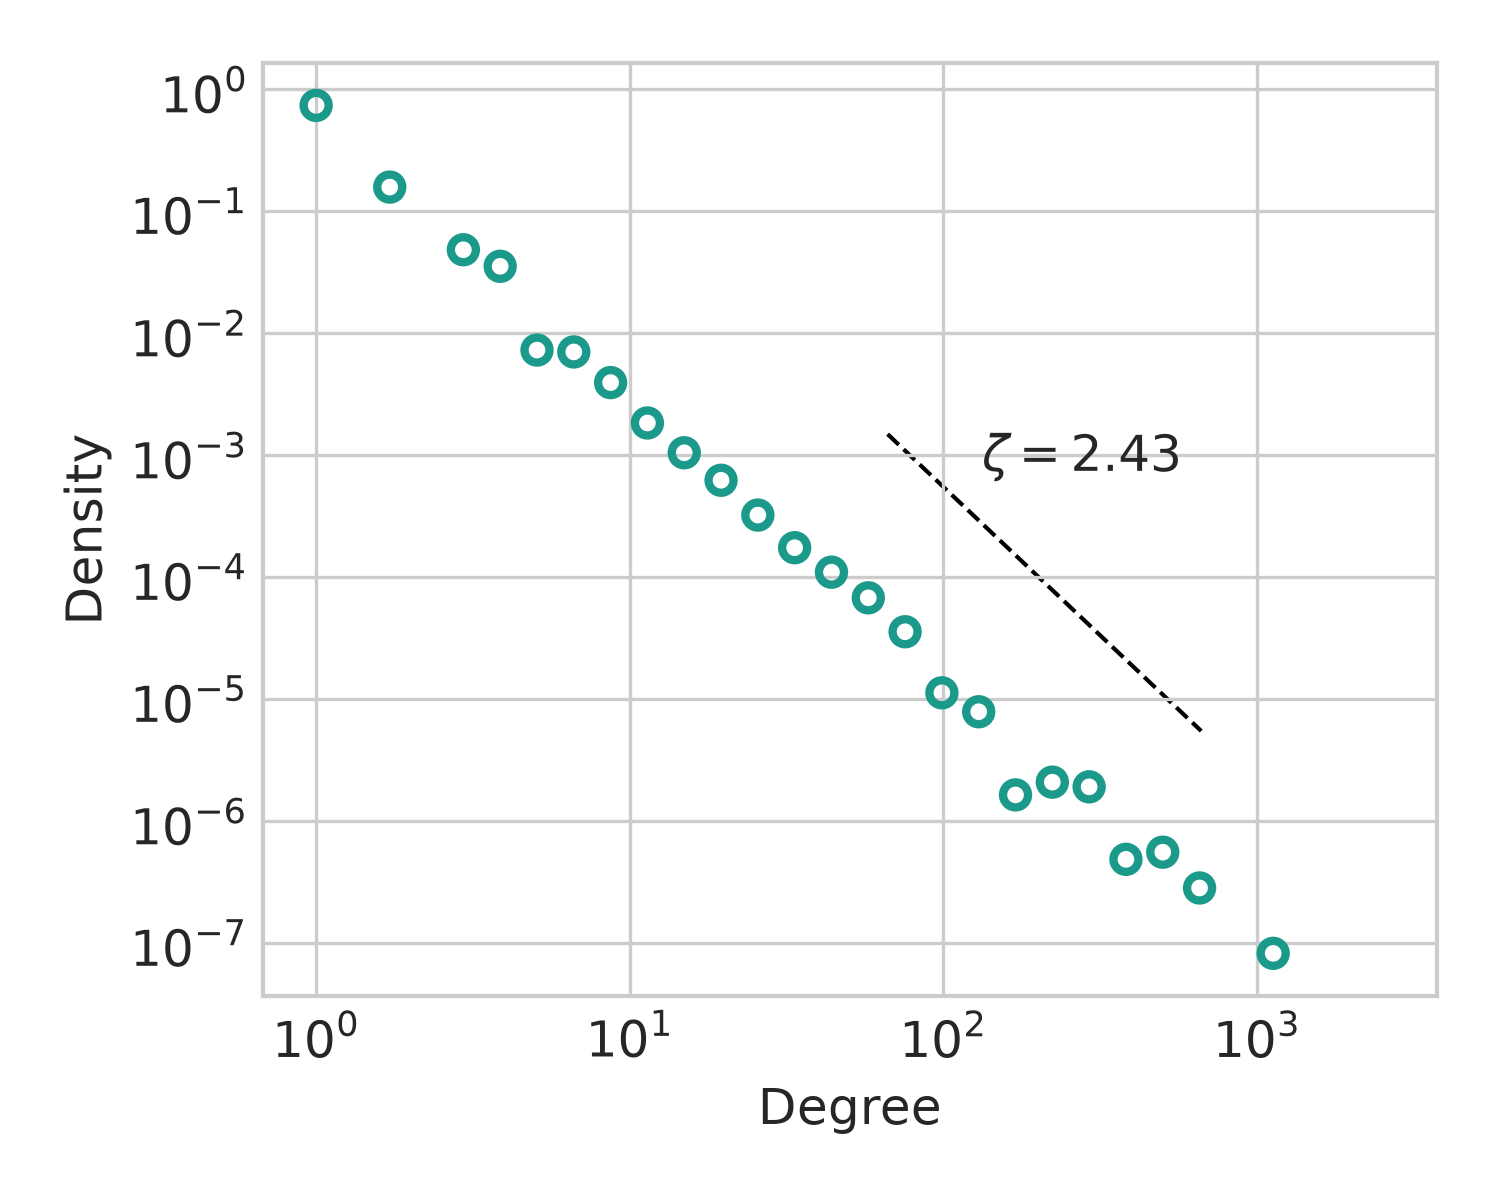
\includegraphics[width=0.5\textwidth]{../fig/degree_distribution.png}
        \caption{
            Degree distribution from model simulation of $10^4$ edges (points) and theoretical power law (line) with exponent given by \Cref{eq:power-law-exponent}. 
            The parameters in this experiment are $\same{\copyrate{}} = 0.7, \opp{\copyrate{}} = 0.3, \same{\extantrate{}} = 0.5, \opp{\extantrate{}} = \opp{\novelrate{}}3, \same{\novelrate{}} = 0.2, \opp{\novelrate{}} = 0.1$. 
            }
        \label{fig:degrees}
    \end{figure}

    \section{\DIFdelbegin \DIFdel{More }\DIFdelend \DIFaddbegin \DIFadd{Additional Details }\DIFaddend on Stochastic Expectation-Maximization (SEM)} \label{sec:sufficient-statistics}

    \subsection{Sufficient Statistics}
        We describe the function \DIFdelbegin \DIFdel{$\sigma$ }\DIFdelend \DIFaddbegin \DIFadd{$\vsigma$ }\DIFaddend from \Cref{sec:sem} which computes the conditional sufficient statistics for the parameters $\paramvector = (\same{\copyrate{}}, \opp{\copyrate{}}, \same{\extantrate{}}, \opp{\extantrate{}}, \same{\novelrate{}}, \opp{\novelrate{}})$ given an observed edge $e$, a candidate parent edge $f$, a candidate seed node $u$, and the node labels $\vz$. 
        Let $z = z_u$ be the label of the seed node $u$. 
        Let $e_z$ be the set of nodes in $e$ with label $z$, and let $f_z$ be the set of nodes in $f$ with label $z$. 
        Then, the sufficient statistics for the parameters $\paramvector$ \DIFaddbegin \DIFadd{\mbox{%DIFAUXCMD
\cite{degrootProbabilityStatistics2012}  }\hskip0pt%DIFAUXCMD
}\DIFaddend are given by
        \begin{align*}
            \DIFdelbegin \DIFdel{\sigma}\DIFdelend \DIFaddbegin \vsigma\DIFaddend (e, f, u, \vz) = \begin{pmatrix}
                \abs{e_z \cap f_z} \\ 
                \abs{f_z} \\ 
                \abs{e_{\bar{z}} \cap f_{\bar{z}}} \\
                \abs{f_{\bar{z}}}  \\ 
                \abs{(e_z \setminus f_z) \cap \at{\nodes}{t}} \\ 
                \abs{(e_{\bar{z}} \setminus f_{\bar{z}})\cap \at{\nodes}{t}} \\
                \abs{e_z \setminus \at{\nodes}{t}} \\
                \abs{e_{\bar{z}} \setminus \at{\nodes}{t}}
            \end{pmatrix}^\top \;.
        \end{align*}
        As descr\DIFaddbegin \DIFadd{i}\DIFaddend bed in \Cref{sec:sem}, the vector $\sufficientstatsvec$ of expected sufficient statistics is computed as a weighted average of \DIFdelbegin \DIFdel{$\sigma(e, f, u, \vz)$ }\DIFdelend \DIFaddbegin \DIFadd{$\vsigma(e, f, u, \vz)$ }\DIFaddend over the belief distribution \DIFdelbegin \DIFdel{$p(f, u | e, \at{\hat{\paramvector}}{\ell})$ }\DIFdelend \DIFaddbegin \DIFadd{$\lik(f, u | e; \at{\hat{\paramvector}}{\ell})$ }\DIFaddend over the latent variables $f$ and $u$.
        Then, the function $g$ which computes the maximum likelihood estimates of the parameters $\paramvector$ from $\sufficientstatsvec$ is given by
        \begin{align*}
            g(\sufficientstatsvec) = \paren{
                \frac{s_1-1}{s_2-1}, 
                \frac{s_3}{s_4}, 
                s_5, 
                s_6, 
                s_7, 
                s_8
            }
             \;.
        \end{align*}

    \subsection{\DIFdelbegin \DIFdel{Implementation Details}\DIFdelend \DIFaddbegin \DIFadd{Learning Rate}\DIFaddend }

        We use an exponentially decaying learning rate for SEM with form \DIFdelbegin \DIFdel{$\lr^{(t)} = \lr^{(0)} \cdot e^{-ct}$}\DIFdelend \DIFaddbegin \DIFadd{$\atalg{\lr}{\epoch} = \atalg{\lr}{0} \cdot e^{-c\epoch}$}\DIFaddend .
        The initial learning rate is set to \DIFdelbegin \DIFdel{$\lr^{(0)} = 0.01$}\DIFdelend \DIFaddbegin \DIFadd{$\atalg{\lr}{0} = 0.01$}\DIFaddend , and the \DIFdelbegin \DIFdel{exponent is defined as }\DIFdelend \DIFaddbegin \DIFadd{decay rate }\DIFaddend $c = 0.001$.
        We initialized the vector of sufficient statistics \DIFdelbegin \DIFdel{$\sufficientstatsvec^{(0)} = (1, 2, 1, 2, 0.5, 0.5, 0.5, 0.5)$}\DIFdelend \DIFaddbegin \DIFadd{$\atalg{\sufficientstatsvec}{0} = (1, 2, 1, 2, 0.5, 0.5, 0.5, 0.5)$}\DIFaddend .
        Other reasonable choices of hyperparameters did not substantially change the results of our experiments.


    \DIFaddbegin \section{\DIFadd{Synthetic SEM Parameter Values}} \label{sec:SEM-appendix}
        \DIFadd{In this section we give more details on the parameter values to demonstrate the performance of SEM on synthetic data in \mbox{%DIFAUXCMD
\Cref{fig:synthetic_sem}}\hskip0pt%DIFAUXCMD
. 
        }\phil{Violet, would be beneficial for you to organize a bit here as well to help the reader correspond values in tables to the figure.}

        \begin{table}[h]
            \caption{\DIFaddFL{Strength of Homophily in Edge Copying}}
            \begin{tabular}{r r r}
                \toprule
                & \DIFaddFL{$\copyrate_+$ }& \DIFaddFL{$\copyrate_-$ }\\
                \midrule
                \DIFaddFL{Weak }&  \DIFaddFL{0.6 }& \DIFaddFL{0.4 }\\
                \DIFaddFL{Strong }& \DIFaddFL{0.9 }& \DIFaddFL{0.2 }\\
                \bottomrule
            \end{tabular}
        \end{table}

        \setlength\tabcolsep{2.5mm}
        \begin{table}[h] 
            \caption{\DIFaddFL{Strength of Homophily in Extant and Novel Node Addition}}\label{tab:sem-heatmap-params}
            \begin{tabular}{l r c c c c}
                && \DIFaddFL{$\extantrate_+$ }& \DIFaddFL{$\extantrate_-$ }& \DIFaddFL{$\novelrate_+$ }& \DIFaddFL{$ \novelrate_-$}\\
                \toprule
                \DIFaddFL{Extant node  }& \DIFaddFL{Strong }& \DIFaddFL{1.0 }& \DIFaddFL{0.8 }& \nullnovsame{} & \nullnovopp{} \\
                \DIFaddFL{addition }& \DIFaddFL{Weak }& \DIFaddFL{2.0 }& \DIFaddFL{0.2 }& \nullnovsame{} & \nullnovopp{} \\
                \midrule
                \DIFaddFL{Novel node }& \DIFaddFL{Strong }& \nullextsame{} & \nullextopp{} & \DIFaddFL{1.0 }& \DIFaddFL{0.8 }\\
                \DIFaddFL{addition }& \DIFaddFL{Weak }& \nullextsame{} & \nullextopp{} & \DIFaddFL{2.0 }& \DIFaddFL{0.2 }\\
                \midrule
                \DIFaddFL{Both }& \DIFaddFL{Strong }& \DIFaddFL{1.0 }& \DIFaddFL{0.8 }& \DIFaddFL{1.0 }& \DIFaddFL{0.8 }\\
                & \DIFaddFL{Weak }& \DIFaddFL{2.0 }& \DIFaddFL{0.2 }& \DIFaddFL{2.0 }& \DIFaddFL{0.2 }\\
                \bottomrule
            \end{tabular}
        \end{table}


        \begin{table}[h]
            \caption{\DIFaddFL{Strength of Copy Mechanism}}
            \begin{tabular}{l r r}
                \toprule
                & \DIFaddFL{$\copyrate_+$ }& \DIFaddFL{$\copyrate_-$ }\\
                \midrule
                \DIFaddFL{Weak }&  \DIFaddFL{0.1 }& \DIFaddFL{0.1 }\\
                \DIFaddFL{Strong }& \DIFaddFL{0.9 }& \DIFaddFL{0.9}\\
                \bottomrule
            \end{tabular}
        \end{table}

        \setlength\tabcolsep{2mm}
        \begin{table}[h]
            \caption{\DIFaddFL{Strength of Extant and Novel Node Addition Mechanisms}}
            \begin{tabular}{l r r r r}
                \toprule
                & \DIFaddFL{$\extantrate_+$ }& \DIFaddFL{$\extantrate_-$ }& \DIFaddFL{$\novelrate_+$ }& \DIFaddFL{$\novelrate_-$}\\
                \midrule
                \DIFaddFL{Both weak }& \DIFaddFL{0.1 }& \DIFaddFL{0.1 }& \DIFaddFL{0.1 }& \DIFaddFL{0.1 }\\
                \DIFaddFL{Strong extant  node mechanism }& \DIFaddFL{2.0 }& \DIFaddFL{2.0 }& \nullnovsame{} & \nullnovopp{} \\
                \DIFaddFL{Weak novel node mechanism }& \nullextsame{} & \nullextopp{} & \DIFaddFL{2.0 }& \DIFaddFL{2.0 }\\
                \DIFaddFL{Both strong }& \DIFaddFL{2.0 }& \DIFaddFL{2.0 }& \DIFaddFL{2.0 }& \DIFaddFL{2.0 }\\
                \bottomrule
            \end{tabular}
        \end{table}






    \DIFaddend \section{Approximation Argument for Simulated Anealing}\label{sec:simulated-annealing-approximation}

        This section provides further detail on the approximation to the likelihood described in \Cref{sec:community-detection} and used in our simulated annealing implementation. 
        The likelihood of an edge $e$ being generated in timestep $t$ can be written 
        \DIFaddbegin \begin{widetext}    
            \DIFaddend \begin{align}
                \DIFdelbegin %DIFDELCMD < \prob%%%
\DIFdelend \DIFaddbegin \lik\DIFaddend (\newedge\DIFdelbegin \DIFdel{|}\DIFdelend \DIFaddbegin \DIFadd{, }\DIFaddend \vz\DIFaddbegin \DIFadd{_\newedge'|}\at{\vz}{t-1}\DIFaddend ;\paramvector) \DIFdelbegin %DIFDELCMD < &%%%
\DIFdelend = \sum_{\substack{\seededge \prec \newedge \\ u\in \seededge}} \DIFdelbegin %DIFDELCMD < \prob%%%
\DIFdelend \DIFaddbegin \lik\DIFaddend (\newedge\DIFaddbegin \DIFadd{, }\vz\DIFadd{_\newedge' }\DIFaddend | \seededge, u, \DIFdelbegin %DIFDELCMD < \vz%%%
\DIFdelend \DIFaddbegin \at{\vz}{t-1}\DIFaddend ; \paramvector) \DIFdelbegin %DIFDELCMD < \\
%DIFDELCMD <                 &%%%
\DIFdelend \DIFaddbegin \lik\DIFadd{(}\seededge\DIFadd{,}\focalnode \DIFadd{| }\at{\edges}{t-1}\DIFadd{, }\at{\vz}{t-1}\DIFadd{; }\paramvector\DIFadd{) }\DIFaddend = \DIFdelbegin \DIFdel{\frac{1}{m_t}}\DIFdelend \DIFaddbegin \DIFadd{\frac{1}{\at{m}{t}}}\DIFaddend \sum_{\seededge \prec \newedge}  \frac{1}{|\seededge|} \sum_{u \in \seededge \cap \newedge} \DIFdelbegin %DIFDELCMD < \prob%%%
\DIFdelend \DIFaddbegin \lik\DIFaddend (\newedge\DIFaddbegin \DIFadd{, }\vz\DIFadd{_\newedge' }\DIFaddend | \seededge, u, \DIFdelbegin %DIFDELCMD < \vz%%%
\DIFdelend \DIFaddbegin \at{\vz}{t-1}\DIFaddend ; \paramvector) \;,
            \end{align} 
        \DIFdelbegin \DIFdel{where $m_t$ }\DIFdelend \DIFaddbegin \end{widetext}
        \DIFadd{where $\at{m}{t}$ }\DIFaddend is the number of edges at time $t$.
        It is helpful to reindex this sum by the size of the intersection $|\seededge \cap \newedge|$ between $\seededge$ and $\newedge$. 
        \begin{align}
            \DIFdelbegin %DIFDELCMD < \prob%%%
\DIFdelend \DIFaddbegin \lik\DIFaddend (\newedge\DIFaddbegin \DIFadd{, }\vz\DIFadd{_\newedge'}\DIFaddend |\vz;\paramvector) &= \sum_{h=0}^{|\newedge|} \sum_{\substack{\seededge \prec \newedge \\ |\seededge \cap \newedge| = k}} \DIFdelbegin \DIFdel{\frac{1}{m_t}}\DIFdelend \DIFaddbegin \DIFadd{\frac{1}{\at{m}{t}}}\DIFaddend \sum_{u \in \seededge \cap \newedge} \frac{1}{|\seededge|} \DIFdelbegin %DIFDELCMD < \prob%%%
\DIFdelend \DIFaddbegin \lik\DIFaddend (\newedge\DIFaddbegin \DIFadd{,}\vz\DIFadd{_\newedge' }\DIFaddend | \seededge, u, \vz; \paramvector) \;.
        \end{align}
        We will now argue that, when $n$ is large, the terms in this sum corresponding to the largest intersections (for which $h = \argmax _{\seededge \prec \newedge} |\seededge \cap \newedge|$) will dominate the likelihood, allowing us to neglect edges $\seededge$ whose intersection with $\newedge$ is smaller.

        Fix edge $\newedge$ generated at time $t$ and candidate parent edge $\seededge$. 
        We subscript $\newedge_z$, $\seededge_z$, and \DIFdelbegin \DIFdel{$\nodes_z^t$ }\DIFdelend \DIFaddbegin \DIFadd{${\at{\nodes}{t}}_z$ }\DIFaddend to denote the subsets of $\newedge$, $\seededge$, and \DIFdelbegin \DIFdel{$\nodes^t$ }\DIFdelend \DIFaddbegin \DIFadd{$\at{\nodes}{t}$ }\DIFaddend with label $z$.
        \DIFaddbegin \DIFadd{We let ${\at{n}{t}}_z = |{\at{\nodes}{t}}_z|$ be the number of nodes of label $z$ at time $t$ and note that ${\at{n}{t}}_0 + {\at{n}{t}}_1 = \at{n}{t}$.
        }\DIFaddend Let $h_z = |(\newedge_z \setminus \seededge_z )\cap \nodes_z^t|$ be the number of extant nodes of label $z$ in $\newedge$.
        Then, the extant node addition process appears in \DIFdelbegin \DIFdel{$\prob(\newedge | \seededge, u, \vz; \paramvector)$ }\DIFdelend \DIFaddbegin \DIFadd{$\lik(\newedge,\vz_\newedge' | \seededge, u, \vz; \paramvector)$ }\DIFaddend as a factor 
        \begin{align}
            E(h_0, h_1) = \DIFdelbegin \DIFdel{\frac{\text{Poisson}(h_{z_u}|\extantrate_+)\times\text{Poisson}(h_{\bar{z}_u}|\extantrate_-)}{\dbinom{|\nodes_{0}^t| - |\seededge_{0}|}{h_{0}}\dbinom{|\nodes_{1}^t| - |\seededge_{1}|}{h_{1}}} }\DIFdelend \DIFaddbegin \DIFadd{\frac{\text{Poisson}(h_{z_u};\extantrate_+)\times\text{Poisson}(h_{\bar{z}_u};\extantrate_-)}{\dbinom{{\at{n}{t}}_0 - |\seededge_{0}|}{h_{0}}\dbinom{{\at{n}{t}}_1 - |\seededge_{1}|}{h_{1}}} }\DIFaddend \;,
        \end{align}
        where the numerator describes the likelihood of adding fixed numbers of extant nodes of each label and the denominator describes the likelihood of selecting the \emph{specific set} of extant nodes from the set of all candidates. 
        Under the assumption that \DIFdelbegin \DIFdel{$n \gg |\seededge|, |\newedge|$}\DIFdelend \DIFaddbegin \DIFadd{$\at{n}{t} \gg |\seededge|, |\newedge|$}\DIFaddend , we can estimate 
        \begin{align}
            \DIFdelbegin %DIFDELCMD < \dbinom{|\nodes_{z}^t| - |\seededge_{z}|}{h_{z}} %%%
\DIFdelend \DIFaddbegin \dbinom{{\at{n}{t}}_z - |\seededge_{z}|}{h_{z}} \DIFaddend \approx \DIFdelbegin \DIFdel{\frac{(|\nodes_z^t|)^{h_z}}{h_z!} }\DIFdelend \DIFaddbegin \DIFadd{\frac{({\at{n}{t}}_z)^{h_z}}{h_z!} }\DIFaddend \approx \DIFdelbegin \DIFdel{\frac{(c_z n)^{h_z}}{h_z!} }\DIFdelend \DIFaddbegin \DIFadd{\frac{(c_z \at{n}{t})^{h_z}}{h_z!} }\DIFaddend \;,
        \end{align}
        where we have defined \DIFdelbegin \DIFdel{$c_z = \frac{|\nodes_z^t|}{n}$ }\DIFdelend \DIFaddbegin \DIFadd{$c_z = \frac{{\at{n}{t}}_z}{\at{n}{t}}$ }\DIFaddend as the fraction of nodes with label $z$. 
        Then, absorbing terms that do not depend on \DIFdelbegin \DIFdel{$n$ }\DIFdelend \DIFaddbegin \DIFadd{$\at{n}{t}$ }\DIFaddend into a constant term $C(h_0, h_1)$, we have 
        \begin{align}
            E(h_0, h_1) &=  C(h_0, h_1) \DIFdelbegin \DIFdel{n}\DIFdelend \DIFaddbegin \at{n}{t}\DIFaddend ^{-h_0 - h_1} + O(\DIFdelbegin \DIFdel{n}\DIFdelend \DIFaddbegin \at{n}{t}\DIFaddend ^{-h_0 - h_1 - 1}) \\ 
                        &= C(h_0, h_1) \DIFdelbegin \DIFdel{n}\DIFdelend \DIFaddbegin \at{n}{t}\DIFaddend ^{-h} + O(\DIFdelbegin \DIFdel{n}\DIFdelend \DIFaddbegin \at{n}{t}\DIFaddend ^{-h - 1}) \;,
        \end{align}
        where \DIFdelbegin \DIFdel{$h = h_0 + h_1 = |(\newedge \setminus \seededge) \cap \nodes^t|$ }\DIFdelend \DIFaddbegin \DIFadd{$h = h_0 + h_1 = |(\newedge \setminus \seededge) \cap \at{\nodes}{t}|$ }\DIFaddend is the total number of extant nodes added to $\newedge$ and 
        \begin{align}
            C(h_0, h_1) &= \frac{\text{Poisson}(h_{z_u}|\extantrate_+)\times\text{Poisson}(h_{\bar{z}_u}|\extantrate_-)}{\frac{(c_0)^{h_0}}{h_0!}\frac{(c_1)^{h_1}}{h_1!}} \;.
        \end{align}
        It follows that \DIFdelbegin \DIFdel{$\prob(\newedge | \seededge, u, \vz; \paramvector)$ }\DIFdelend \DIFaddbegin \DIFadd{$\lik(\newedge,\vz_\newedge' | \seededge, u, \vz; \paramvector)$ }\DIFaddend is of order \DIFdelbegin \DIFdel{$O(n^{-h})$ as $n$ }\DIFdelend \DIFaddbegin \DIFadd{$O(\at{n}{t}^{-h})$ as $\at{n}{t}$ }\DIFaddend grows large, where \DIFdelbegin \DIFdel{$h$ }\DIFdelend \DIFaddbegin \DIFadd{$h = h_0 + h_1$ }\DIFaddend is the number of extant nodes added to $\newedge$.
        Terms corresponding to choices of $\seededge$ for which $h$ is larger (of which there may be up to approximately \DIFdelbegin \DIFdel{$m$}\DIFdelend \DIFaddbegin \DIFadd{$\at{m}{t}$}\DIFaddend ) decay quickly \DIFdelbegin \DIFdel{for large$n$}\DIFdelend \DIFaddbegin \DIFadd{as $\at{n}{t}$ grows large}\DIFaddend . 
        We therefore have 
        \DIFaddbegin \begin{widetext}
            \DIFaddend \begin{align}
                \DIFdelbegin %DIFDELCMD < \prob%%%
\DIFdelend \DIFaddbegin \lik\DIFaddend (\newedge\DIFaddbegin \DIFadd{,}\vz\DIFadd{_\newedge'}\DIFaddend |\vz;\paramvector) &= \sum_{\substack{\seededge \prec \newedge \\ |\seededge \cap \newedge| = h'}} \DIFdelbegin \DIFdel{\frac{1}{m_t}}\DIFdelend \DIFaddbegin \DIFadd{\frac{1}{\at{m}{t}}}\DIFaddend \sum_{u \in \seededge \cap \newedge} \frac{1}{|\seededge|}  \DIFdelbegin %DIFDELCMD < \prob%%%
\DIFdelend \DIFaddbegin \lik\DIFaddend (\newedge\DIFaddbegin \DIFadd{,}\vz\DIFadd{_\newedge' }\DIFaddend | \seededge, u, \vz; \paramvector)  + \DIFdelbegin \DIFdel{mO}\DIFdelend \DIFaddbegin \at{m}{t}\DIFadd{O}\DIFaddend (\DIFdelbegin \DIFdel{n}\DIFdelend \DIFaddbegin \at{n}{t}\DIFaddend ^{-h'-1}) \label{eq:sa-approx}
            \end{align}
        \DIFdelbegin \DIFdel{where $h' = \min_{\seededge \prec \newedge} |(\newedge \setminus \seededge) \cap \nodes^t|$ }\DIFdelend \DIFaddbegin \end{widetext}
        \DIFadd{where $h' = \min_{\seededge \prec \newedge} |(\newedge \setminus \seededge) \cap \at{\nodes}{t}|$ }\DIFaddend is the minimum number of extant nodes added to $\newedge$ across all choices of $\seededge$.

        This argument suggests that, when \DIFdelbegin \DIFdel{$n$ }\DIFdelend \DIFaddbegin \DIFadd{$\at{n}{t}$ }\DIFaddend is relatively large in relation to \DIFdelbegin \DIFdel{$m$}\DIFdelend \DIFaddbegin \DIFadd{$\at{m}{t}$}\DIFaddend , the likelihood of $\newedge$ is dominated by terms corresponding to choices of $\seededge$ for which the number of extant nodes added to $\newedge$ is small.
        There are two limitations to this argument in the context of empirical data sets. 
        First, it may be the case that only a small number of candidate parent edges $\seededge$ have \DIFdelbegin \DIFdel{small $h$}\DIFdelend \DIFaddbegin \DIFadd{large intersections with $\newedge$ }\DIFaddend , which may lead to a poor approximation of the likelihood when we evaluate only a small number of corresponding terms.
        Second, several of our data sets have \DIFdelbegin \DIFdel{$m$ }\DIFdelend \DIFaddbegin \DIFadd{$\at{m}{t}$ }\DIFaddend large in relation to \DIFdelbegin \DIFdel{$n$}\DIFdelend \DIFaddbegin \DIFadd{$\at{n}{t}$}\DIFaddend , making it dubious to neglect the error term. 
        We therefore introduce two variations to our approximation heuristic: 
        \begin{itemize}
            \item \textbf{Top $j$ heuristic}: Rather than evaluate only terms for $f$ for which \DIFaddbegin \DIFadd{the number of extant nodes }\DIFaddend $h$ \DIFaddbegin \DIFadd{to be added }\DIFaddend is minimal, we evaluate terms for the top $j$ choices of $\seededge$ with the smallest \DIFaddbegin \DIFadd{values of }\DIFaddend $h$.
            \item \textbf{Batch normalization}: Rather than normalizing by \DIFdelbegin \DIFdel{$\frac{1}{m_t}$ }\DIFdelend \DIFaddbegin \DIFadd{$\frac{1}{\at{m}{t}}$ }\DIFaddend in \cref{eq:sa-approx}, we normalize by the number of  \DIFdelbegin \DIFdel{$\seededge$ choices }\DIFdelend \DIFaddbegin \DIFadd{choices for $\seededge$ that }\DIFaddend we evaluate for a specific $\newedge$. 
            This may be $j$ under the top $j$ heuristic, or it may be the number of $\seededge$ choices with $h$ equal to the minimum $h'$ if we do not use the top $j$ heuristic. 
            Letting $\mathcal{F}_\newedge$ be the set of \DIFaddbegin \DIFadd{seed edges }\DIFaddend $\seededge$ \DIFdelbegin \DIFdel{choices we evaluate for a specific }\DIFdelend \DIFaddbegin \DIFadd{evaluated for a given }\DIFaddend $\newedge$ \DIFaddbegin \DIFadd{under the top $j$ or similar heuristic}\DIFaddend , our approximation is 
            \begin{align}
                \DIFdelbegin %DIFDELCMD < \tilde{\prob}%%%
\DIFdelend \DIFaddbegin \tilde{\lik}\DIFaddend (\newedge\DIFaddbegin \DIFadd{,}\vz\DIFadd{_\newedge'}\DIFaddend |\vz;\paramvector) &=\frac{1}{|\mathcal{F}_\newedge|}\sum_{\substack{\seededge \in \mathcal{F}_\newedge}} \sum_{u \in \seededge \cap \newedge} \frac{1}{|\seededge|}  \DIFdelbegin %DIFDELCMD < \prob%%%
\DIFdelend \DIFaddbegin \lik\DIFaddend (\newedge\DIFaddbegin \DIFadd{,}\vz\DIFadd{_\newedge' }\DIFaddend | \seededge, u, \vz; \paramvector)\;. 
            \end{align}
            \DIFdelbegin \DIFdel{Meaning the }\DIFdelend \DIFaddbegin \DIFadd{The }\DIFaddend approximate likelihood of the \DIFdelbegin \DIFdel{entire $\hypergraph$ is }\DIFdelend \DIFaddbegin \DIFadd{complete data set is then 
            }\DIFaddend \begin{align}
                 \DIFdelbegin %DIFDELCMD < \tilde{\prob} %%%
\DIFdelend \DIFaddbegin \tilde{\lik} \DIFaddend (\hypergraph, \vz; \paramvector )&= \prod_{\newedge \in \edges}\DIFdelbegin %DIFDELCMD < \tilde{\prob}%%%
\DIFdelend \DIFaddbegin \tilde{\lik}\DIFaddend (\newedge\DIFaddbegin \DIFadd{,}\vz\DIFadd{_\newedge'}\DIFaddend |\vz;\paramvector)\DIFaddbegin \DIFadd{\;. }\DIFaddend \label{eq:sa-approx-2}
            \end{align}
        \end{itemize}
        It is important to note that the batch normalization \cref{eq:sa-approx-2} tends to overestimate the likelihood, since we have restricted ourselves to an average of high-probability seed-edges. 
        For the purposes of simulated annealing, this is not a major problem since we are only interested in the relative likelihood of different labelings $\vz$ and not the absolute \DIFaddbegin \DIFadd{scale of }\DIFaddend likelihood.

    \section{Simulated Annealing for Community Detection}\label{sec:simulated-annealing-algorithm-spec}
        We \DIFaddbegin \DIFadd{now }\DIFaddend describe the simulated annealing algorithm \DIFdelbegin \DIFdel{implementation in detail.
        Define the number of epochs for the }\DIFdelend \DIFaddbegin \DIFadd{from \mbox{%DIFAUXCMD
\Cref{sec:community-detection} }\hskip0pt%DIFAUXCMD
in greater detail. 
        Our custom learning schedule uses the first epoch to set the absolute scale of the acceptance probability decay, which we therefore describe as a separate algorithm (\mbox{%DIFAUXCMD
\Cref{algocf:simulated_annealing_first_epoch}}\hskip0pt%DIFAUXCMD
).
        We then proceed to the main }\DIFaddend simulated annealing algorithm \DIFdelbegin \DIFdel{$A = 20$.
        Let $a(\epoch)$ be the probability that the simulated annealing algorithm accepts a change on labels that lowers the approximated likelihood
        }\DIFdelend \DIFaddbegin \DIFadd{(\mbox{%DIFAUXCMD
\Cref{algocf:simulated_annealing}}\hskip0pt%DIFAUXCMD
), which uses the scale of acceptance probability decay $\sigma_\hypergraph$ computed in the first epoch to set the acceptance probability for label flips in subsequent epochs.
        We only allow the probability to begin to decay after the first four epochs in order to encourage exploration of the label space. 
        }\DIFaddend 

        \begin{algorithm}[H]
            \begin{algorithmic}
                \caption{\DIFdelbegin \texttt{\DIFdel{SimulatedAnnealing}}%DIFAUXCMD
\DIFdel{$(\hypergraph, \theta)$}\DIFdelend \DIFaddbegin \texttt{\DIFadd{SimulatedAnnealingFirstEpoch}}\DIFadd{$(\hypergraph, \paramvector)$}\DIFaddend }\DIFdelbegin %DIFDELCMD < \label{algocf:simulated_annealing}
%DIFDELCMD <                 \Require{Hypergraph $\hypergraph$, parameters $\paramvector$, number of epochs $A$}
%DIFDELCMD <                 \Ensure{Label set $\vz$, approximation of the true labels $\vz^*$}
%DIFDELCMD <                 %%%
\DIFdelend \DIFaddbegin \label{algocf:simulated_annealing_first_epoch}
                \Require{Hypergraph $\hypergraph$ with $n$ nodes, parameters $\paramvector$}
                \Ensure{Estimate $\sigma_\hypergraph$ for scale of acceptance probability decay, updated label set $\hat{\vz}$}
                \DIFaddend \State Sample \DIFdelbegin \DIFdel{$\vz \sim \text{Uniform}(\{0,1\})^{n}$
                }\DIFdelend \DIFaddbegin \DIFadd{$\hat{\vz} \sim \text{Uniform}(\{0,1\})^{n}$ }\Comment{initialization}
                \DIFaddend \State \DIFdelbegin \DIFdel{$\Delta \mathcal{L} \gets \emptyset$
                }\DIFdelend \DIFaddbegin \DIFadd{$\vdelta \gets \vzero \in \R^n$ }\Comment{initialize vector of log-likelihood differences}
                \For{$\step = 1$ to $n$}
                    \DIFaddend \State \DIFdelbegin \DIFdel{$\sigma_\hypergraph \gets 0$
                }%DIFDELCMD < \For{$\epoch = 0$ to $A$}
%DIFDELCMD <                     \For{$\step = 0$ to $n$}
%DIFDELCMD <                         \State %%%
\DIFdelend Sample $j$ $\sim$ Uniform(\DIFdelbegin \DIFdel{$\{0,...,n-1\}$}\DIFdelend \DIFaddbegin \DIFadd{$\{1,...,n\}$}\DIFaddend )
                    \State \DIFdelbegin \DIFdel{$\vz^\prime$ }\DIFdelend \DIFaddbegin \DIFadd{$\hat{\vz}^\prime$ }\DIFaddend $\gets$ \DIFdelbegin \DIFdel{$\vz$
                        }\DIFdelend \DIFaddbegin \DIFadd{$\hat{\vz}$
                    }\DIFaddend \State $z^\prime_j\gets1-z^\prime_j$
                    \State \DIFdelbegin \DIFdel{$\Delta E \gets \log \overset{\sim}{\prob}(\hypergraph, \vz^\prime | \paramvector) - \log \overset{\sim}{\prob}(\hypergraph, \vz | \paramvector)$
                        }%DIFDELCMD < \If{ $\epoch = 0$}
%DIFDELCMD <                             %%%
\DIFdelend \DIFaddbegin \DIFadd{$\vdelta_\tau \gets \log \tilde{\lik}(\hypergraph, \hat{\vz}^\prime ; \paramvector) - \log \tilde{\lik}(\hypergraph, \hat{\vz} ; \paramvector)$ }\Comment{populate $\vdelta$ with log-likelihood differences}
                \EndFor
                \DIFaddend \State \DIFdelbegin \DIFdel{$\Delta \mathcal{L} \gets \Delta \mathcal{L} \cup \{\Delta E\}$
                        }%DIFDELCMD < \EndIf
%DIFDELCMD <                         \If{$\sigma_\hypergraph = 0 \And \epoch > 0$}
%DIFDELCMD <                                 %%%
\DIFdelend \DIFaddbegin \DIFadd{$\sigma_\hypergraph\gets \sigma(\vdelta)$
                }\DIFaddend \State \DIFdelbegin \DIFdel{$\sigma_\hypergraph\gets \sigma(\Delta \mathcal{L})$
                            }%DIFDELCMD < \EndIf
%DIFDELCMD <                         \If{$\Delta E>0$}
%DIFDELCMD <                             %%%
\DIFdelend \DIFaddbegin \Return \DIFadd{$\sigma_\hypergraph$, $\hat{\vz}$
            }\end{algorithmic}
        \end{algorithm}

        \DIFadd{Here, $\sigma(\vdelta)$ is the empirical variance
        }\begin{align}
            \DIFadd{\sigma(\vdelta) = \sqrt{\frac{\sum_{i = 1}^n \delta_i^2 - (\frac{1}{n}\sum_{i=1}^n \delta_i)^2}{n-1}}\;.
        }\end{align}


        \begin{algorithm}[H]
            \begin{algorithmic}
                \caption{\texttt{\DIFadd{SimulatedAnnealing}}\DIFadd{$(\hypergraph, \paramvector)$}}\label{algocf:simulated_annealing}
                \Require{Hypergraph $\hypergraph$, parameters $\paramvector$, number of epochs $\maxepochs$}
                \Ensure{Label set $\hat{\vz}$, estimate of true labels $\vz$}
                \DIFaddend \State \DIFdelbegin \DIFdel{$\vz \gets\vz^\prime$
                        }%DIFDELCMD < \Else
%DIFDELCMD <                             \State %%%
\DIFdel{$a(\epoch)$ }\DIFdelend \DIFaddbegin \DIFadd{$\sigma_\hypergraph$, $\hat{\vz}$ }\DIFaddend $\gets$ \DIFdelbegin \DIFdel{1
                            }\DIFdelend \DIFaddbegin \texttt{\DIFadd{SimulatedAnnealingFirstEpoch}}\DIFadd{$(\hypergraph, \paramvector)$
                }\For{$\epoch = 1$ to $\maxepochs$}
                    \For{$\step = 1$ to $n$}
                        \DIFaddend \State \DIFdelbegin \DIFdel{$\zeta_a$ }\DIFdelend \DIFaddbegin \DIFadd{Sample $j$ $\sim$ Uniform($\{1,...,n\}$)
                        }\State \DIFadd{$\hat{\vz}^\prime$ }\DIFaddend $\gets$ \DIFdelbegin \DIFdel{$\Delta E/\sigma_\hypergraph$
                            }%DIFDELCMD < \If{$1 \leq \epoch \leq 4$}
%DIFDELCMD <                                 %%%
\DIFdelend \DIFaddbegin \DIFadd{$\hat{\vz}$
                        }\DIFaddend \State \DIFdelbegin \DIFdel{$a(\epoch)$ }\DIFdelend \DIFaddbegin \DIFadd{$z^\prime_j\gets1-z^\prime_j$
                        }\State \DIFadd{$\delta \gets \log \tilde{\lik}(\hypergraph, \hat{\vz}^\prime ; \paramvector) - \log \tilde{\lik}(\hypergraph, \hat{\vz} ; \paramvector)$
                        }\If{$\delta>0$}
                            \State \DIFadd{$\hat{\vz} \gets\hat{\vz}^\prime$
                        }\Else
                            \If{$2 \leq \epoch \leq 5$}
                                \State \DIFadd{$\atalg{\acceptprob}{\epoch}$ }\DIFaddend $\gets$ \DIFdelbegin \DIFdel{Normal($\zeta_a|\mu = 0, \sigma=2$)
                            }%DIFDELCMD < \ElsIf{5 $\leq \epoch$}
%DIFDELCMD <                                 %%%
\DIFdelend \DIFaddbegin \DIFadd{$\mathrm{Gaussian}(\delta;\mu = 0, \sigma=2\sigma_\hypergraph)$
                            }\ElsIf{6 $\leq \epoch$}
                                \DIFaddend \State \DIFdelbegin \DIFdel{$a(\epoch)$ }\DIFdelend \DIFaddbegin \DIFadd{$\atalg{\acceptprob}{\epoch}$ }\DIFaddend $\gets$ \DIFdelbegin \DIFdel{Normal($\zeta_a|\mu = 0, \sigma=2(1 - \frac{\epoch}{A}))$
                            }\DIFdelend \DIFaddbegin \DIFadd{$\mathrm{Gaussian}(\delta;\mu = 0, \sigma=2(1 - \frac{\epoch}{\maxepochs})\sigma_\hypergraph)$
                            }\DIFaddend \EndIf
                            \State Sample $x \sim \text{Uniform}(0,1)$
                            \DIFdelbegin %DIFDELCMD < \If{$B > x$} 
%DIFDELCMD <                                 %%%
\DIFdelend \DIFaddbegin \If{$x < \atalg{\acceptprob}{\epoch}$} 
                                \DIFaddend \State \DIFdelbegin \DIFdel{$\vz \gets \vz^\prime$
                            }\DIFdelend \DIFaddbegin \DIFadd{$\hat{\vz} \gets \hat{\vz}^\prime$
                            }\DIFaddend \EndIf
                        \EndIf
                    \EndFor
                \EndFor
                \State \Return\DIFdelbegin \DIFdel{$\vz$
            }\DIFdelend \DIFaddbegin \DIFadd{$\hat{\vz}$
            }\DIFaddend \end{algorithmic}
        \end{algorithm}
        \DIFdelbegin %DIFDELCMD < \frannie{Can our $\Delta \mathcal{L}$ be a set like this?  Will this not accept duplicates?}
%DIFDELCMD < %%%
\DIFdelend 

    
    \DIFdelbegin \DIFdel{Here, 
        }\begin{align*}
            \DIFdel{\sigma(\Delta \mathcal{L}) = \sqrt{\frac{\sum_{\delta  \in \Delta \mathcal{L}} \delta^2 - (\frac{1}{|\Delta \mathcal{L}|}\sum_{\delta \in \Delta \mathcal{L}} \delta)^2}{|\Delta \mathcal{L}|-1}}
        }\end{align*}%DIFAUXCMD
%DIFDELCMD <     

%DIFDELCMD <     %%%
\DIFdelend \section{Simulated Annealing Illustration}

        \begin{figure*}[h]
            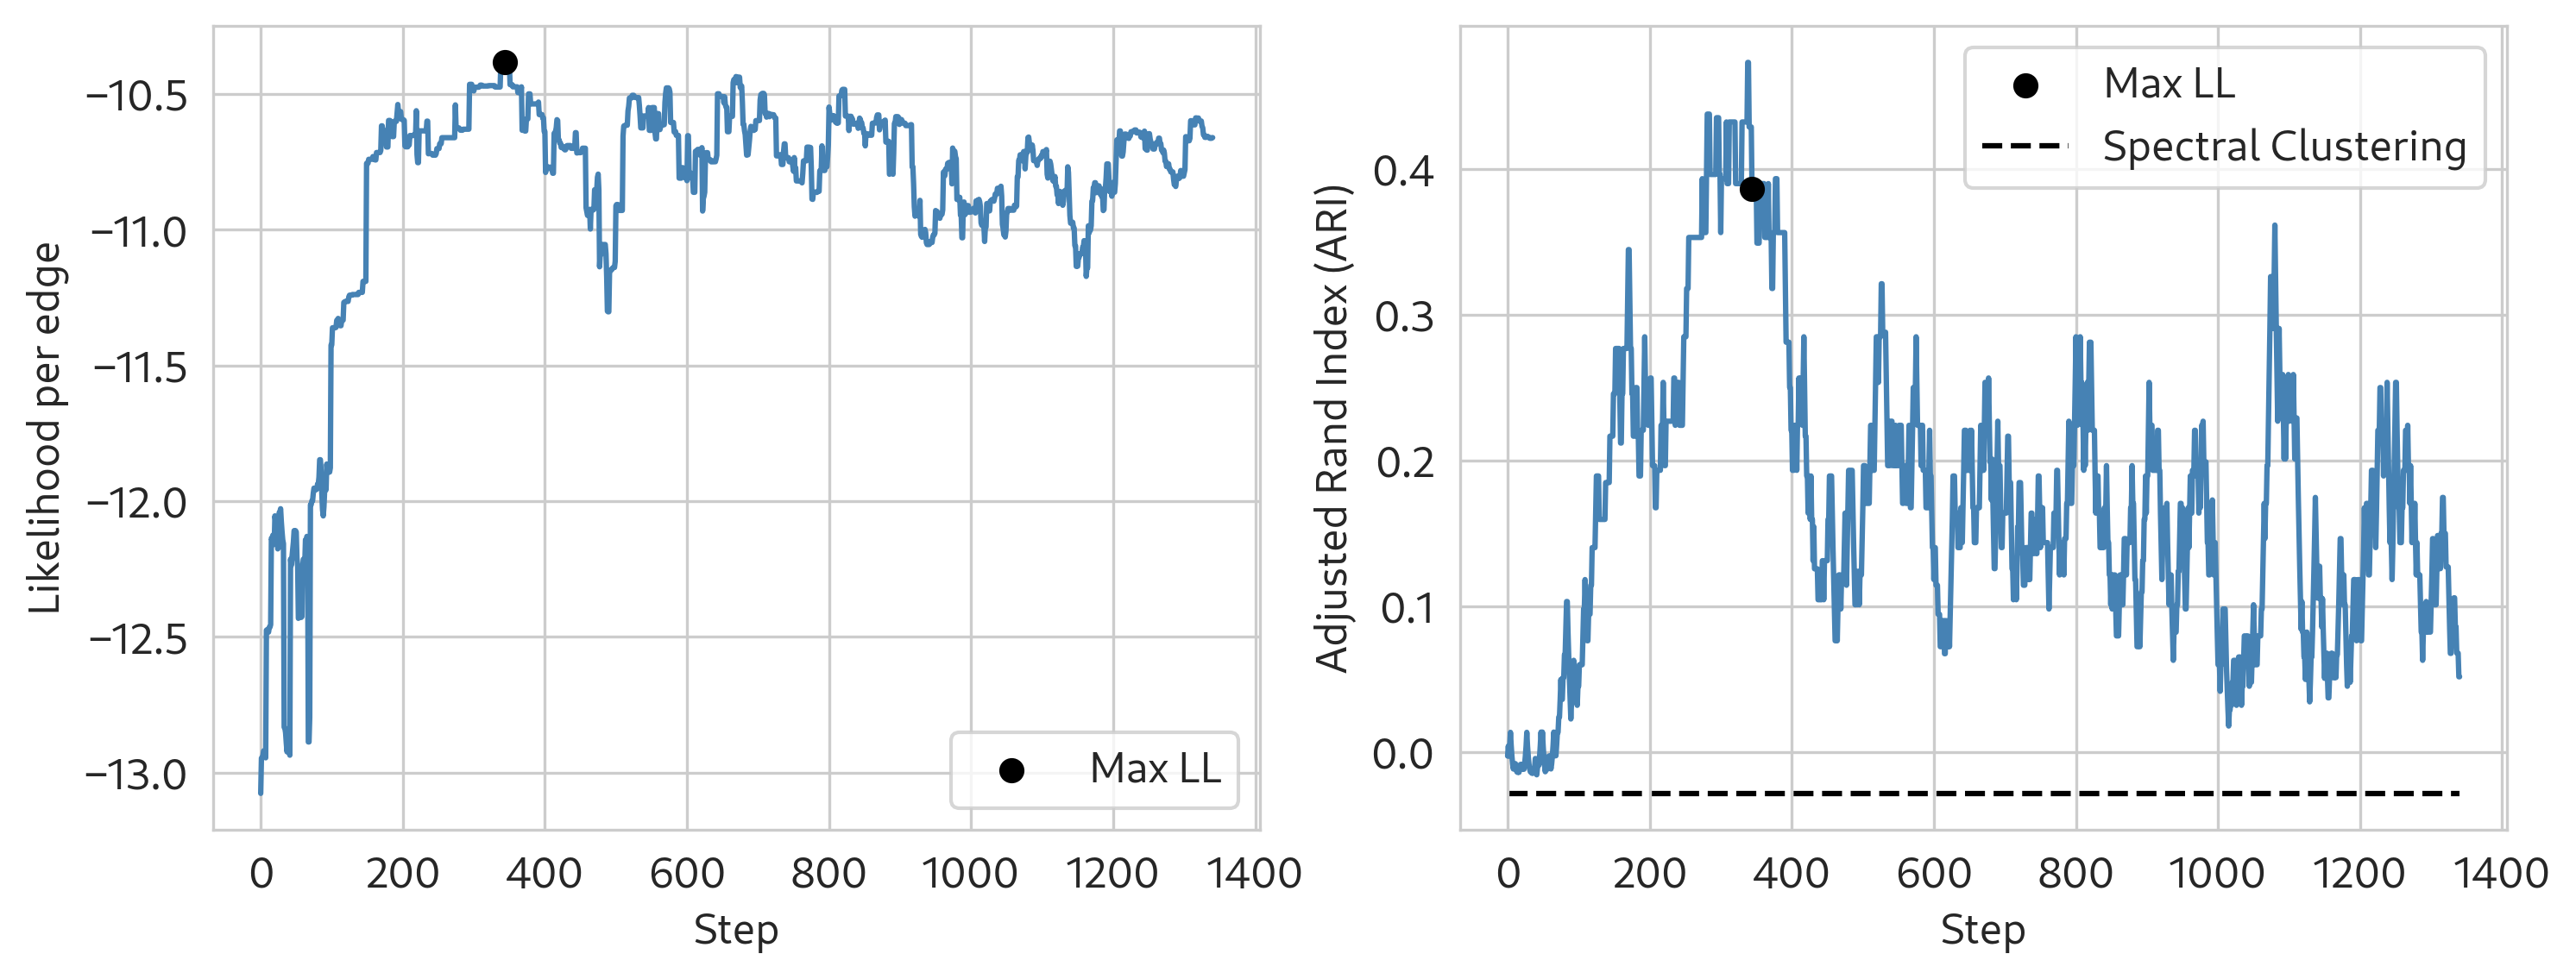
\includegraphics[width=1.0\textwidth]{../fig/community-detection-learning-progress.png}
            \caption{
                Illustrative run of simulated annealing for community detection in a hypergraph generated from our model.
                The dashed line on the right shows the ARI achieved by Laplacian spectral clustering applied to the weighted dyadic graph projection.  
                \DIFaddbeginFL \DIFaddFL{Solid point gives the highest likelihood and corresponding ARI achieved by simulated annealing over the course of the run. 
            }\DIFaddendFL }
        \end{figure*}
        \DIFdelbegin %DIFDELCMD < 

%DIFDELCMD <         %%%
\DIFdelend \DIFaddbegin \DIFadd{We provide simple illustration of a single run of simulated annealing as described in \mbox{%DIFAUXCMD
\Cref{algocf:simulated_annealing_first_epoch,algocf:simulated_annealing} }\hskip0pt%DIFAUXCMD
for community detection in a hypergraph generated from our model.
        }\DIFaddend In this simulation, we generated a simple hypergraph according to our model with \simannviznumnodes{} nodes and \simannviznumedges{} edges.
        Running simulated annealing for \simannviznumsteps{} steps, we obtained a maximum log-likelihood of \simannvizmaxll{} nats per edge with an Adjusted Rand Index (ARI) against ground-truth of \simannvizmaxllari{}. 
        \DIFdelbegin %DIFDELCMD < \frannie{What does nats per edge mean?}
%DIFDELCMD <         %%%
\DIFdel{Greedy modularity maximization }\DIFdelend \DIFaddbegin \DIFadd{Laplacian spectral clustering }\DIFaddend as implemented in the Python package \texttt{networkx} \cite{networkx} obtained an ARI of \DIFdelbegin %DIFDELCMD < \simannvizmodularityari{}%%%
\DIFdelend \DIFaddbegin \simannvizspectralari{}\DIFaddend .
        The parameters for the model used to generate the hypergraph are 
        \begin{align*}
            \DIFdelbegin %DIFDELCMD < \same{\copyrate{}} &%%%
\DIFdelend \DIFaddbegin \paramvector \DIFaddend = \DIFdelbegin %DIFDELCMD < \simannvizsamecopyrate{} \\ 
%DIFDELCMD <             %%%
\DIFdelend \DIFaddbegin \DIFadd{(}\same{\copyrate{}}\DIFadd{, }\DIFaddend \opp{\copyrate{}}\DIFdelbegin %DIFDELCMD < &%%%
\DIFdel{= }%DIFDELCMD < \simannvizoppcopyrate{} \\ 
%DIFDELCMD <             %%%
\DIFdelend \DIFaddbegin \DIFadd{, }\DIFaddend \same{\extantrate{}}\DIFdelbegin %DIFDELCMD < &%%%
\DIFdel{= }%DIFDELCMD < \simannvizsameextantrate{} \\ 
%DIFDELCMD <             %%%
\DIFdelend \DIFaddbegin \DIFadd{, }\DIFaddend \opp{\extantrate{}}\DIFdelbegin %DIFDELCMD < &%%%
\DIFdel{= }%DIFDELCMD < \simannvizoppextantrate{} \\ 
%DIFDELCMD <             %%%
\DIFdelend \DIFaddbegin \DIFadd{, }\DIFaddend \same{\novelrate{}}\DIFdelbegin %DIFDELCMD < &%%%
\DIFdel{= }%DIFDELCMD < \simannvizsamenovelrate{} \\ 
%DIFDELCMD <             %%%
\DIFdelend \DIFaddbegin \DIFadd{, }\DIFaddend \opp{\novelrate{}}\DIFdelbegin %DIFDELCMD < &%%%
\DIFdelend \DIFaddbegin \DIFadd{) }\DIFaddend = \DIFaddbegin \DIFadd{(}\simannvizsamecopyrate{}\DIFadd{, }\simannvizoppcopyrate{}\DIFadd{, }\simannvizsameextantrate{}\DIFadd{, }\simannvizoppextantrate{}\DIFadd{, }\simannvizsamenovelrate{}\DIFadd{, }\DIFaddend \simannvizoppnovelrate{}\DIFaddbegin \DIFadd{)}\DIFaddend \;.
        \end{align*}
        \DIFdelbegin \DIFdel{The guessed parameters used to compute the likelihood during simulated annealing are 
        }\begin{align*}
            \DIFdel{\same{\hat\copyrate{}} }&\DIFdel{= \simannvizsamecopyrateguess{} }\\ 
            \DIFdel{\opp{\hat\copyrate{}} }&\DIFdel{= \simannvizoppcopyrateguess{} }\\ 
            \DIFdel{\same{\hat\extantrate{}} }&\DIFdel{= \simannvizsameextantrateguess{} }\\ 
            \DIFdel{\opp{\hat\extantrate{}} }&\DIFdel{= \simannvizoppextantrateguess{} }\\ 
            \DIFdel{\same{\hat\novelrate{}} }&\DIFdel{= \simannvizsamenovelrateguess{} }\\ 
            \DIFdel{\opp{\hat\novelrate{}} }&\DIFdel{= \simannvizoppnovelrateguess{}\;. 
        }\end{align*}%DIFAUXCMD
%DIFDELCMD <         \frannie{Params are the same here, should we just say they are used to generate the hypergraph and recover the community structure?}
%DIFDELCMD <     

%DIFDELCMD <     %%%
\section{\DIFdel{More Simulated Annealing on Synthetic Data}}
    %DIFAUXCMD
\addtocounter{section}{-1}%DIFAUXCMD
%DIFDELCMD < \frannie{Empty as is.  I liked the heatmap, but understand if it doesn't justify its space!}
%DIFDELCMD < 

%DIFDELCMD < %%%
%DIF <      \begin{figure*}
%DIF <      \includegraphics[width=\textwidth]{../fig/community-synthetic-data-viz-supplementary.png}
%DIF <      \caption{
%DIF <          Community detection results on synthetic data.
%DIF <          Each pixel represents \synthrepetitions{} independent hypergraphs generated from our model with \synthtimesteps{} timesteps. 
%DIF <          In each heatmap, we vary $\same{\copyrate{}}$ and $\opp{\copyrate{}}$, holding $(\same{\extantrate{}}, \opp{\extantrate{}}, \same{\novelrate{}}, \opp{\novelrate{}}) =
%DIF <          (\synthfixedlambdaplus, \synthfixedlambdaminus, \synthfixedgammaplus, \synthfixedgammaminus)$. 
%DIF <      } \label{fig:community-synthetic}
%DIF <  \end{figure*}
%DIFDELCMD < 

%DIFDELCMD <     %%%
\section{\DIFdel{Synthetic SEM Parameter Values}} %DIFAUXCMD
\addtocounter{section}{-1}%DIFAUXCMD
%DIFDELCMD < \label{sec:SEM-appendix}
%DIFDELCMD <     \frannie{Fix formatting here.  Not sure if the section is finished as is}
%DIFDELCMD < 

%DIFDELCMD <     \begin{table}[h]
%DIFDELCMD <         %%%
%DIFDELCMD < \caption{%
{%DIFAUXCMD
\DIFdelFL{Strength of Homophily in Edge Copying}}
        %DIFAUXCMD
%DIFDELCMD < \begin{tabular}{r r r}
%DIFDELCMD <             \toprule
%DIFDELCMD <             & %%%
\DIFdelFL{$\copyrate_+$ }%DIFDELCMD < & %%%
\DIFdelFL{$\copyrate_-$ }%DIFDELCMD < \\
%DIFDELCMD <             \midrule
%DIFDELCMD <             %%%
\DIFdelFL{Weak }%DIFDELCMD < &  %%%
\DIFdelFL{0.6 }%DIFDELCMD < & %%%
\DIFdelFL{0.4 }%DIFDELCMD < \\
%DIFDELCMD <             %%%
\DIFdelFL{Strong }%DIFDELCMD < & %%%
\DIFdelFL{0.9 }%DIFDELCMD < & %%%
\DIFdelFL{0.2 }%DIFDELCMD < \\
%DIFDELCMD <             \bottomrule
%DIFDELCMD <         \end{tabular}
%DIFDELCMD <     \end{table}
%DIFDELCMD < 

%DIFDELCMD <     \setlength\tabcolsep{2.5mm}
%DIFDELCMD <     \begin{table}[h] 
%DIFDELCMD <         %%%
%DIFDELCMD < \caption{%
{%DIFAUXCMD
\DIFdelFL{Strength of Homophily in Extant and Novel Node Addition}}%DIFAUXCMD
%DIFDELCMD < \label{tab:sem-heatmap-params}
%DIFDELCMD <         \begin{tabular}{l r c c c c}
%DIFDELCMD <             && %%%
\DIFdelFL{$\extantrate_+$ }%DIFDELCMD < & %%%
\DIFdelFL{$\extantrate_-$ }%DIFDELCMD < & %%%
\DIFdelFL{$\novelrate_+$ }%DIFDELCMD < & %%%
\DIFdelFL{$ \novelrate_-$}%DIFDELCMD < \\
%DIFDELCMD <             \toprule
%DIFDELCMD <             %%%
\DIFdelFL{Extant node  }%DIFDELCMD < & %%%
\DIFdelFL{Strong }%DIFDELCMD < & %%%
\DIFdelFL{1.0 }%DIFDELCMD < & %%%
\DIFdelFL{0.8 }%DIFDELCMD < & \nullnovsame{} & \nullnovopp{} \\
%DIFDELCMD <             %%%
\DIFdelFL{addition }%DIFDELCMD < & %%%
\DIFdelFL{Weak }%DIFDELCMD < & %%%
\DIFdelFL{2.0 }%DIFDELCMD < & %%%
\DIFdelFL{0.2 }%DIFDELCMD < & \nullnovsame{} & \nullnovopp{} \\
%DIFDELCMD <             \midrule
%DIFDELCMD <             %%%
\DIFdelFL{Novel node }%DIFDELCMD < & %%%
\DIFdelFL{Strong }%DIFDELCMD < & \nullextsame{} & \nullextopp{} & %%%
\DIFdelFL{1.0 }%DIFDELCMD < & %%%
\DIFdelFL{0.8 }%DIFDELCMD < \\
%DIFDELCMD <              %%%
\DIFdelFL{addition }%DIFDELCMD < & %%%
\DIFdelFL{Weak }%DIFDELCMD < & \nullextsame{} & \nullextopp{} & %%%
\DIFdelFL{2.0 }%DIFDELCMD < & %%%
\DIFdelFL{0.2 }%DIFDELCMD < \\
%DIFDELCMD <             \midrule
%DIFDELCMD <             %%%
\DIFdelFL{Both }%DIFDELCMD < & %%%
\DIFdelFL{Strong }%DIFDELCMD < & %%%
\DIFdelFL{1.0 }%DIFDELCMD < & %%%
\DIFdelFL{0.8 }%DIFDELCMD < & %%%
\DIFdelFL{1.0 }%DIFDELCMD < & %%%
\DIFdelFL{0.8 }%DIFDELCMD < \\
%DIFDELCMD <             & %%%
\DIFdelFL{Weak }%DIFDELCMD < & %%%
\DIFdelFL{2.0 }%DIFDELCMD < & %%%
\DIFdelFL{0.2 }%DIFDELCMD < & %%%
\DIFdelFL{2.0 }%DIFDELCMD < & %%%
\DIFdelFL{0.2 }%DIFDELCMD < \\
%DIFDELCMD <             \bottomrule
%DIFDELCMD <         \end{tabular}
%DIFDELCMD <     \end{table}
%DIFDELCMD < 

%DIFDELCMD <     \begin{table}[h]
%DIFDELCMD <         %%%
%DIFDELCMD < \caption{%
{%DIFAUXCMD
\DIFdelFL{Strength of Copy Mechanism}}
        %DIFAUXCMD
%DIFDELCMD < \begin{tabular}{l r r}
%DIFDELCMD <             \toprule
%DIFDELCMD <             & %%%
\DIFdelFL{$\copyrate_+$ }%DIFDELCMD < & %%%
\DIFdelFL{$\copyrate_-$ }%DIFDELCMD < \\
%DIFDELCMD <             \midrule
%DIFDELCMD <             %%%
\DIFdelFL{Weak }%DIFDELCMD < &  %%%
\DIFdelFL{0.1 }%DIFDELCMD < & %%%
\DIFdelFL{0.1 }%DIFDELCMD < \\
%DIFDELCMD <             %%%
\DIFdelFL{Strong }%DIFDELCMD < & %%%
\DIFdelFL{0.9 }%DIFDELCMD < & %%%
\DIFdelFL{0.9}%DIFDELCMD < \\
%DIFDELCMD <             \bottomrule
%DIFDELCMD <         \end{tabular}
%DIFDELCMD <     \end{table}
%DIFDELCMD < 

%DIFDELCMD <     \setlength\tabcolsep{2mm}
%DIFDELCMD <     \begin{table}[h]
%DIFDELCMD <         %%%
%DIFDELCMD < \caption{%
{%DIFAUXCMD
\DIFdelFL{Strength of Extant and Novel Node Addition Mechanisms}}
        %DIFAUXCMD
%DIFDELCMD < \begin{tabular}{l r r r r}
%DIFDELCMD <             \toprule
%DIFDELCMD <             & %%%
\DIFdelFL{$\extantrate_+$ }%DIFDELCMD < & %%%
\DIFdelFL{$\extantrate_-$ }%DIFDELCMD < & %%%
\DIFdelFL{$\novelrate_+$ }%DIFDELCMD < & %%%
\DIFdelFL{$\novelrate_-$}%DIFDELCMD < \\
%DIFDELCMD <             \midrule
%DIFDELCMD <             %%%
\DIFdelFL{Both weak }%DIFDELCMD < & %%%
\DIFdelFL{0.1 }%DIFDELCMD < & %%%
\DIFdelFL{0.1 }%DIFDELCMD < & %%%
\DIFdelFL{0.1 }%DIFDELCMD < & %%%
\DIFdelFL{0.1 }%DIFDELCMD < \\
%DIFDELCMD <             %%%
\DIFdelFL{Strong extant  node mechanism }%DIFDELCMD < & %%%
\DIFdelFL{2.0 }%DIFDELCMD < & %%%
\DIFdelFL{2.0 }%DIFDELCMD < & \nullnovsame{} & \nullnovopp{} \\
%DIFDELCMD <             %%%
\DIFdelFL{Weak novel node mechanism }%DIFDELCMD < & \nullextsame{} & \nullextopp{} & %%%
\DIFdelFL{2.0 }%DIFDELCMD < & %%%
\DIFdelFL{2.0 }%DIFDELCMD < \\
%DIFDELCMD <             %%%
\DIFdelFL{Both strong }%DIFDELCMD < & %%%
\DIFdelFL{2.0 }%DIFDELCMD < & %%%
\DIFdelFL{2.0 }%DIFDELCMD < & %%%
\DIFdelFL{2.0 }%DIFDELCMD < & %%%
\DIFdelFL{2.0 }%DIFDELCMD < \\
%DIFDELCMD <             \bottomrule
%DIFDELCMD <         \end{tabular}
%DIFDELCMD <     \end{table}
%DIFDELCMD < %%%
\DIFdelend \DIFaddbegin \DIFadd{For the purposes of this illustration we perform community detection under the Nishimori condition, using a guess $\hat{\paramvector}$ equal to the true parameters $\paramvector$ used to generate the hypergraph.
        }\DIFaddend 

    
    \end{document}